\documentclass[11pt]{article}

    \usepackage[breakable]{tcolorbox}
    \usepackage{parskip} % Stop auto-indenting (to mimic markdown behaviour)

    \usepackage{iftex}
    \ifPDFTeX
    	\usepackage[T1]{fontenc}
    	\usepackage{mathpazo}
    \else
    	\usepackage{fontspec}
    \fi

    % Basic figure setup, for now with no caption control since it's done
    % automatically by Pandoc (which extracts ![](path) syntax from Markdown).
    \usepackage{graphicx}
    % Maintain compatibility with old templates. Remove in nbconvert 6.0
    \let\Oldincludegraphics\includegraphics
    % Ensure that by default, figures have no caption (until we provide a
    % proper Figure object with a Caption API and a way to capture that
    % in the conversion process - todo).
    \usepackage{caption}
    \DeclareCaptionFormat{nocaption}{}
    \captionsetup{format=nocaption,aboveskip=0pt,belowskip=0pt}

    \usepackage{float}
    \floatplacement{figure}{H} % forces figures to be placed at the correct location
    \usepackage{xcolor} % Allow colors to be defined
    \usepackage{enumerate} % Needed for markdown enumerations to work
    \usepackage{geometry} % Used to adjust the document margins
    \usepackage{amsmath} % Equations
    \usepackage{amssymb} % Equations
    \usepackage{textcomp} % defines textquotesingle
    % Hack from http://tex.stackexchange.com/a/47451/13684:
    \AtBeginDocument{%
        \def\PYZsq{\textquotesingle}% Upright quotes in Pygmentized code
    }
    \usepackage{upquote} % Upright quotes for verbatim code
    \usepackage{eurosym} % defines \euro
    \usepackage[mathletters]{ucs} % Extended unicode (utf-8) support
    \usepackage{fancyvrb} % verbatim replacement that allows latex
    \usepackage{grffile} % extends the file name processing of package graphics
                         % to support a larger range
    \makeatletter % fix for old versions of grffile with XeLaTeX
    \@ifpackagelater{grffile}{2019/11/01}
    {
      % Do nothing on new versions
    }
    {
      \def\Gread@@xetex#1{%
        \IfFileExists{"\Gin@base".bb}%
        {\Gread@eps{\Gin@base.bb}}%
        {\Gread@@xetex@aux#1}%
      }
    }
    \makeatother
    \usepackage[Export]{adjustbox} % Used to constrain images to a maximum size
    \adjustboxset{max size={0.9\linewidth}{0.9\paperheight}}

    % The hyperref package gives us a pdf with properly built
    % internal navigation ('pdf bookmarks' for the table of contents,
    % internal cross-reference links, web links for URLs, etc.)
    \usepackage{hyperref}
    % The default LaTeX title has an obnoxious amount of whitespace. By default,
    % titling removes some of it. It also provides customization options.
    \usepackage{titling}
    \usepackage{longtable} % longtable support required by pandoc >1.10
    \usepackage{booktabs}  % table support for pandoc > 1.12.2
    \usepackage[inline]{enumitem} % IRkernel/repr support (it uses the enumerate* environment)
    \usepackage[normalem]{ulem} % ulem is needed to support strikethroughs (\sout)
                                % normalem makes italics be italics, not underlines
    \usepackage{mathrsfs}



    % Colors for the hyperref package
    \definecolor{urlcolor}{rgb}{0,.145,.698}
    \definecolor{linkcolor}{rgb}{.71,0.21,0.01}
    \definecolor{citecolor}{rgb}{.12,.54,.11}

    % ANSI colors
    \definecolor{ansi-black}{HTML}{3E424D}
    \definecolor{ansi-black-intense}{HTML}{282C36}
    \definecolor{ansi-red}{HTML}{E75C58}
    \definecolor{ansi-red-intense}{HTML}{B22B31}
    \definecolor{ansi-green}{HTML}{00A250}
    \definecolor{ansi-green-intense}{HTML}{007427}
    \definecolor{ansi-yellow}{HTML}{DDB62B}
    \definecolor{ansi-yellow-intense}{HTML}{B27D12}
    \definecolor{ansi-blue}{HTML}{208FFB}
    \definecolor{ansi-blue-intense}{HTML}{0065CA}
    \definecolor{ansi-magenta}{HTML}{D160C4}
    \definecolor{ansi-magenta-intense}{HTML}{A03196}
    \definecolor{ansi-cyan}{HTML}{60C6C8}
    \definecolor{ansi-cyan-intense}{HTML}{258F8F}
    \definecolor{ansi-white}{HTML}{C5C1B4}
    \definecolor{ansi-white-intense}{HTML}{A1A6B2}
    \definecolor{ansi-default-inverse-fg}{HTML}{FFFFFF}
    \definecolor{ansi-default-inverse-bg}{HTML}{000000}

    % common color for the border for error outputs.
    \definecolor{outerrorbackground}{HTML}{FFDFDF}

    % commands and environments needed by pandoc snippets
    % extracted from the output of `pandoc -s`
    \providecommand{\tightlist}{%
      \setlength{\itemsep}{0pt}\setlength{\parskip}{0pt}}
    \DefineVerbatimEnvironment{Highlighting}{Verbatim}{commandchars=\\\{\}}
    % Add ',fontsize=\small' for more characters per line
    \newenvironment{Shaded}{}{}
    \newcommand{\KeywordTok}[1]{\textcolor[rgb]{0.00,0.44,0.13}{\textbf{{#1}}}}
    \newcommand{\DataTypeTok}[1]{\textcolor[rgb]{0.56,0.13,0.00}{{#1}}}
    \newcommand{\DecValTok}[1]{\textcolor[rgb]{0.25,0.63,0.44}{{#1}}}
    \newcommand{\BaseNTok}[1]{\textcolor[rgb]{0.25,0.63,0.44}{{#1}}}
    \newcommand{\FloatTok}[1]{\textcolor[rgb]{0.25,0.63,0.44}{{#1}}}
    \newcommand{\CharTok}[1]{\textcolor[rgb]{0.25,0.44,0.63}{{#1}}}
    \newcommand{\StringTok}[1]{\textcolor[rgb]{0.25,0.44,0.63}{{#1}}}
    \newcommand{\CommentTok}[1]{\textcolor[rgb]{0.38,0.63,0.69}{\textit{{#1}}}}
    \newcommand{\OtherTok}[1]{\textcolor[rgb]{0.00,0.44,0.13}{{#1}}}
    \newcommand{\AlertTok}[1]{\textcolor[rgb]{1.00,0.00,0.00}{\textbf{{#1}}}}
    \newcommand{\FunctionTok}[1]{\textcolor[rgb]{0.02,0.16,0.49}{{#1}}}
    \newcommand{\RegionMarkerTok}[1]{{#1}}
    \newcommand{\ErrorTok}[1]{\textcolor[rgb]{1.00,0.00,0.00}{\textbf{{#1}}}}
    \newcommand{\NormalTok}[1]{{#1}}

    % Additional commands for more recent versions of Pandoc
    \newcommand{\ConstantTok}[1]{\textcolor[rgb]{0.53,0.00,0.00}{{#1}}}
    \newcommand{\SpecialCharTok}[1]{\textcolor[rgb]{0.25,0.44,0.63}{{#1}}}
    \newcommand{\VerbatimStringTok}[1]{\textcolor[rgb]{0.25,0.44,0.63}{{#1}}}
    \newcommand{\SpecialStringTok}[1]{\textcolor[rgb]{0.73,0.40,0.53}{{#1}}}
    \newcommand{\ImportTok}[1]{{#1}}
    \newcommand{\DocumentationTok}[1]{\textcolor[rgb]{0.73,0.13,0.13}{\textit{{#1}}}}
    \newcommand{\AnnotationTok}[1]{\textcolor[rgb]{0.38,0.63,0.69}{\textbf{\textit{{#1}}}}}
    \newcommand{\CommentVarTok}[1]{\textcolor[rgb]{0.38,0.63,0.69}{\textbf{\textit{{#1}}}}}
    \newcommand{\VariableTok}[1]{\textcolor[rgb]{0.10,0.09,0.49}{{#1}}}
    \newcommand{\ControlFlowTok}[1]{\textcolor[rgb]{0.00,0.44,0.13}{\textbf{{#1}}}}
    \newcommand{\OperatorTok}[1]{\textcolor[rgb]{0.40,0.40,0.40}{{#1}}}
    \newcommand{\BuiltInTok}[1]{{#1}}
    \newcommand{\ExtensionTok}[1]{{#1}}
    \newcommand{\PreprocessorTok}[1]{\textcolor[rgb]{0.74,0.48,0.00}{{#1}}}
    \newcommand{\AttributeTok}[1]{\textcolor[rgb]{0.49,0.56,0.16}{{#1}}}
    \newcommand{\InformationTok}[1]{\textcolor[rgb]{0.38,0.63,0.69}{\textbf{\textit{{#1}}}}}
    \newcommand{\WarningTok}[1]{\textcolor[rgb]{0.38,0.63,0.69}{\textbf{\textit{{#1}}}}}


    % Define a nice break command that doesn't care if a line doesn't already
    % exist.
    \def\br{\hspace*{\fill} \\* }
    % Math Jax compatibility definitions
    \def\gt{>}
    \def\lt{<}
    \let\Oldtex\TeX
    \let\Oldlatex\LaTeX
    \renewcommand{\TeX}{\textrm{\Oldtex}}
    \renewcommand{\LaTeX}{\textrm{\Oldlatex}}
    % Document parameters
    % Document title
    \title{Mathematics for Neuroscience - An introduction }
    \date{}




% Pygments definitions
\makeatletter
\def\PY@reset{\let\PY@it=\relax \let\PY@bf=\relax%
    \let\PY@ul=\relax \let\PY@tc=\relax%
    \let\PY@bc=\relax \let\PY@ff=\relax}
\def\PY@tok#1{\csname PY@tok@#1\endcsname}
\def\PY@toks#1+{\ifx\relax#1\empty\else%
    \PY@tok{#1}\expandafter\PY@toks\fi}
\def\PY@do#1{\PY@bc{\PY@tc{\PY@ul{%
    \PY@it{\PY@bf{\PY@ff{#1}}}}}}}
\def\PY#1#2{\PY@reset\PY@toks#1+\relax+\PY@do{#2}}

\@namedef{PY@tok@w}{\def\PY@tc##1{\textcolor[rgb]{0.73,0.73,0.73}{##1}}}
\@namedef{PY@tok@c}{\let\PY@it=\textit\def\PY@tc##1{\textcolor[rgb]{0.25,0.50,0.50}{##1}}}
\@namedef{PY@tok@cp}{\def\PY@tc##1{\textcolor[rgb]{0.74,0.48,0.00}{##1}}}
\@namedef{PY@tok@k}{\let\PY@bf=\textbf\def\PY@tc##1{\textcolor[rgb]{0.00,0.50,0.00}{##1}}}
\@namedef{PY@tok@kp}{\def\PY@tc##1{\textcolor[rgb]{0.00,0.50,0.00}{##1}}}
\@namedef{PY@tok@kt}{\def\PY@tc##1{\textcolor[rgb]{0.69,0.00,0.25}{##1}}}
\@namedef{PY@tok@o}{\def\PY@tc##1{\textcolor[rgb]{0.40,0.40,0.40}{##1}}}
\@namedef{PY@tok@ow}{\let\PY@bf=\textbf\def\PY@tc##1{\textcolor[rgb]{0.67,0.13,1.00}{##1}}}
\@namedef{PY@tok@nb}{\def\PY@tc##1{\textcolor[rgb]{0.00,0.50,0.00}{##1}}}
\@namedef{PY@tok@nf}{\def\PY@tc##1{\textcolor[rgb]{0.00,0.00,1.00}{##1}}}
\@namedef{PY@tok@nc}{\let\PY@bf=\textbf\def\PY@tc##1{\textcolor[rgb]{0.00,0.00,1.00}{##1}}}
\@namedef{PY@tok@nn}{\let\PY@bf=\textbf\def\PY@tc##1{\textcolor[rgb]{0.00,0.00,1.00}{##1}}}
\@namedef{PY@tok@ne}{\let\PY@bf=\textbf\def\PY@tc##1{\textcolor[rgb]{0.82,0.25,0.23}{##1}}}
\@namedef{PY@tok@nv}{\def\PY@tc##1{\textcolor[rgb]{0.10,0.09,0.49}{##1}}}
\@namedef{PY@tok@no}{\def\PY@tc##1{\textcolor[rgb]{0.53,0.00,0.00}{##1}}}
\@namedef{PY@tok@nl}{\def\PY@tc##1{\textcolor[rgb]{0.63,0.63,0.00}{##1}}}
\@namedef{PY@tok@ni}{\let\PY@bf=\textbf\def\PY@tc##1{\textcolor[rgb]{0.60,0.60,0.60}{##1}}}
\@namedef{PY@tok@na}{\def\PY@tc##1{\textcolor[rgb]{0.49,0.56,0.16}{##1}}}
\@namedef{PY@tok@nt}{\let\PY@bf=\textbf\def\PY@tc##1{\textcolor[rgb]{0.00,0.50,0.00}{##1}}}
\@namedef{PY@tok@nd}{\def\PY@tc##1{\textcolor[rgb]{0.67,0.13,1.00}{##1}}}
\@namedef{PY@tok@s}{\def\PY@tc##1{\textcolor[rgb]{0.73,0.13,0.13}{##1}}}
\@namedef{PY@tok@sd}{\let\PY@it=\textit\def\PY@tc##1{\textcolor[rgb]{0.73,0.13,0.13}{##1}}}
\@namedef{PY@tok@si}{\let\PY@bf=\textbf\def\PY@tc##1{\textcolor[rgb]{0.73,0.40,0.53}{##1}}}
\@namedef{PY@tok@se}{\let\PY@bf=\textbf\def\PY@tc##1{\textcolor[rgb]{0.73,0.40,0.13}{##1}}}
\@namedef{PY@tok@sr}{\def\PY@tc##1{\textcolor[rgb]{0.73,0.40,0.53}{##1}}}
\@namedef{PY@tok@ss}{\def\PY@tc##1{\textcolor[rgb]{0.10,0.09,0.49}{##1}}}
\@namedef{PY@tok@sx}{\def\PY@tc##1{\textcolor[rgb]{0.00,0.50,0.00}{##1}}}
\@namedef{PY@tok@m}{\def\PY@tc##1{\textcolor[rgb]{0.40,0.40,0.40}{##1}}}
\@namedef{PY@tok@gh}{\let\PY@bf=\textbf\def\PY@tc##1{\textcolor[rgb]{0.00,0.00,0.50}{##1}}}
\@namedef{PY@tok@gu}{\let\PY@bf=\textbf\def\PY@tc##1{\textcolor[rgb]{0.50,0.00,0.50}{##1}}}
\@namedef{PY@tok@gd}{\def\PY@tc##1{\textcolor[rgb]{0.63,0.00,0.00}{##1}}}
\@namedef{PY@tok@gi}{\def\PY@tc##1{\textcolor[rgb]{0.00,0.63,0.00}{##1}}}
\@namedef{PY@tok@gr}{\def\PY@tc##1{\textcolor[rgb]{1.00,0.00,0.00}{##1}}}
\@namedef{PY@tok@ge}{\let\PY@it=\textit}
\@namedef{PY@tok@gs}{\let\PY@bf=\textbf}
\@namedef{PY@tok@gp}{\let\PY@bf=\textbf\def\PY@tc##1{\textcolor[rgb]{0.00,0.00,0.50}{##1}}}
\@namedef{PY@tok@go}{\def\PY@tc##1{\textcolor[rgb]{0.53,0.53,0.53}{##1}}}
\@namedef{PY@tok@gt}{\def\PY@tc##1{\textcolor[rgb]{0.00,0.27,0.87}{##1}}}
\@namedef{PY@tok@err}{\def\PY@bc##1{{\setlength{\fboxsep}{\string -\fboxrule}\fcolorbox[rgb]{1.00,0.00,0.00}{1,1,1}{\strut ##1}}}}
\@namedef{PY@tok@kc}{\let\PY@bf=\textbf\def\PY@tc##1{\textcolor[rgb]{0.00,0.50,0.00}{##1}}}
\@namedef{PY@tok@kd}{\let\PY@bf=\textbf\def\PY@tc##1{\textcolor[rgb]{0.00,0.50,0.00}{##1}}}
\@namedef{PY@tok@kn}{\let\PY@bf=\textbf\def\PY@tc##1{\textcolor[rgb]{0.00,0.50,0.00}{##1}}}
\@namedef{PY@tok@kr}{\let\PY@bf=\textbf\def\PY@tc##1{\textcolor[rgb]{0.00,0.50,0.00}{##1}}}
\@namedef{PY@tok@bp}{\def\PY@tc##1{\textcolor[rgb]{0.00,0.50,0.00}{##1}}}
\@namedef{PY@tok@fm}{\def\PY@tc##1{\textcolor[rgb]{0.00,0.00,1.00}{##1}}}
\@namedef{PY@tok@vc}{\def\PY@tc##1{\textcolor[rgb]{0.10,0.09,0.49}{##1}}}
\@namedef{PY@tok@vg}{\def\PY@tc##1{\textcolor[rgb]{0.10,0.09,0.49}{##1}}}
\@namedef{PY@tok@vi}{\def\PY@tc##1{\textcolor[rgb]{0.10,0.09,0.49}{##1}}}
\@namedef{PY@tok@vm}{\def\PY@tc##1{\textcolor[rgb]{0.10,0.09,0.49}{##1}}}
\@namedef{PY@tok@sa}{\def\PY@tc##1{\textcolor[rgb]{0.73,0.13,0.13}{##1}}}
\@namedef{PY@tok@sb}{\def\PY@tc##1{\textcolor[rgb]{0.73,0.13,0.13}{##1}}}
\@namedef{PY@tok@sc}{\def\PY@tc##1{\textcolor[rgb]{0.73,0.13,0.13}{##1}}}
\@namedef{PY@tok@dl}{\def\PY@tc##1{\textcolor[rgb]{0.73,0.13,0.13}{##1}}}
\@namedef{PY@tok@s2}{\def\PY@tc##1{\textcolor[rgb]{0.73,0.13,0.13}{##1}}}
\@namedef{PY@tok@sh}{\def\PY@tc##1{\textcolor[rgb]{0.73,0.13,0.13}{##1}}}
\@namedef{PY@tok@s1}{\def\PY@tc##1{\textcolor[rgb]{0.73,0.13,0.13}{##1}}}
\@namedef{PY@tok@mb}{\def\PY@tc##1{\textcolor[rgb]{0.40,0.40,0.40}{##1}}}
\@namedef{PY@tok@mf}{\def\PY@tc##1{\textcolor[rgb]{0.40,0.40,0.40}{##1}}}
\@namedef{PY@tok@mh}{\def\PY@tc##1{\textcolor[rgb]{0.40,0.40,0.40}{##1}}}
\@namedef{PY@tok@mi}{\def\PY@tc##1{\textcolor[rgb]{0.40,0.40,0.40}{##1}}}
\@namedef{PY@tok@il}{\def\PY@tc##1{\textcolor[rgb]{0.40,0.40,0.40}{##1}}}
\@namedef{PY@tok@mo}{\def\PY@tc##1{\textcolor[rgb]{0.40,0.40,0.40}{##1}}}
\@namedef{PY@tok@ch}{\let\PY@it=\textit\def\PY@tc##1{\textcolor[rgb]{0.25,0.50,0.50}{##1}}}
\@namedef{PY@tok@cm}{\let\PY@it=\textit\def\PY@tc##1{\textcolor[rgb]{0.25,0.50,0.50}{##1}}}
\@namedef{PY@tok@cpf}{\let\PY@it=\textit\def\PY@tc##1{\textcolor[rgb]{0.25,0.50,0.50}{##1}}}
\@namedef{PY@tok@c1}{\let\PY@it=\textit\def\PY@tc##1{\textcolor[rgb]{0.25,0.50,0.50}{##1}}}
\@namedef{PY@tok@cs}{\let\PY@it=\textit\def\PY@tc##1{\textcolor[rgb]{0.25,0.50,0.50}{##1}}}

\def\PYZbs{\char`\\}
\def\PYZus{\char`\_}
\def\PYZob{\char`\{}
\def\PYZcb{\char`\}}
\def\PYZca{\char`\^}
\def\PYZam{\char`\&}
\def\PYZlt{\char`\<}
\def\PYZgt{\char`\>}
\def\PYZsh{\char`\#}
\def\PYZpc{\char`\%}
\def\PYZdl{\char`\$}
\def\PYZhy{\char`\-}
\def\PYZsq{\char`\'}
\def\PYZdq{\char`\"}
\def\PYZti{\char`\~}
% for compatibility with earlier versions
\def\PYZat{@}
\def\PYZlb{[}
\def\PYZrb{]}
\makeatother


    % For linebreaks inside Verbatim environment from package fancyvrb.
    \makeatletter
        \newbox\Wrappedcontinuationbox
        \newbox\Wrappedvisiblespacebox
        \newcommand*\Wrappedvisiblespace {\textcolor{red}{\textvisiblespace}}
        \newcommand*\Wrappedcontinuationsymbol {\textcolor{red}{\llap{\tiny$\m@th\hookrightarrow$}}}
        \newcommand*\Wrappedcontinuationindent {3ex }
        \newcommand*\Wrappedafterbreak {\kern\Wrappedcontinuationindent\copy\Wrappedcontinuationbox}
        % Take advantage of the already applied Pygments mark-up to insert
        % potential linebreaks for TeX processing.
        %        {, <, #, %, $, ' and ": go to next line.
        %        _, }, ^, &, >, - and ~: stay at end of broken line.
        % Use of \textquotesingle for straight quote.
        \newcommand*\Wrappedbreaksatspecials {%
            \def\PYGZus{\discretionary{\char`\_}{\Wrappedafterbreak}{\char`\_}}%
            \def\PYGZob{\discretionary{}{\Wrappedafterbreak\char`\{}{\char`\{}}%
            \def\PYGZcb{\discretionary{\char`\}}{\Wrappedafterbreak}{\char`\}}}%
            \def\PYGZca{\discretionary{\char`\^}{\Wrappedafterbreak}{\char`\^}}%
            \def\PYGZam{\discretionary{\char`\&}{\Wrappedafterbreak}{\char`\&}}%
            \def\PYGZlt{\discretionary{}{\Wrappedafterbreak\char`\<}{\char`\<}}%
            \def\PYGZgt{\discretionary{\char`\>}{\Wrappedafterbreak}{\char`\>}}%
            \def\PYGZsh{\discretionary{}{\Wrappedafterbreak\char`\#}{\char`\#}}%
            \def\PYGZpc{\discretionary{}{\Wrappedafterbreak\char`\%}{\char`\%}}%
            \def\PYGZdl{\discretionary{}{\Wrappedafterbreak\char`\$}{\char`\$}}%
            \def\PYGZhy{\discretionary{\char`\-}{\Wrappedafterbreak}{\char`\-}}%
            \def\PYGZsq{\discretionary{}{\Wrappedafterbreak\textquotesingle}{\textquotesingle}}%
            \def\PYGZdq{\discretionary{}{\Wrappedafterbreak\char`\"}{\char`\"}}%
            \def\PYGZti{\discretionary{\char`\~}{\Wrappedafterbreak}{\char`\~}}%
        }
        % Some characters . , ; ? ! / are not pygmentized.
        % This macro makes them "active" and they will insert potential linebreaks
        \newcommand*\Wrappedbreaksatpunct {%
            \lccode`\~`\.\lowercase{\def~}{\discretionary{\hbox{\char`\.}}{\Wrappedafterbreak}{\hbox{\char`\.}}}%
            \lccode`\~`\,\lowercase{\def~}{\discretionary{\hbox{\char`\,}}{\Wrappedafterbreak}{\hbox{\char`\,}}}%
            \lccode`\~`\;\lowercase{\def~}{\discretionary{\hbox{\char`\;}}{\Wrappedafterbreak}{\hbox{\char`\;}}}%
            \lccode`\~`\:\lowercase{\def~}{\discretionary{\hbox{\char`\:}}{\Wrappedafterbreak}{\hbox{\char`\:}}}%
            \lccode`\~`\?\lowercase{\def~}{\discretionary{\hbox{\char`\?}}{\Wrappedafterbreak}{\hbox{\char`\?}}}%
            \lccode`\~`\!\lowercase{\def~}{\discretionary{\hbox{\char`\!}}{\Wrappedafterbreak}{\hbox{\char`\!}}}%
            \lccode`\~`\/\lowercase{\def~}{\discretionary{\hbox{\char`\/}}{\Wrappedafterbreak}{\hbox{\char`\/}}}%
            \catcode`\.\active
            \catcode`\,\active
            \catcode`\;\active
            \catcode`\:\active
            \catcode`\?\active
            \catcode`\!\active
            \catcode`\/\active
            \lccode`\~`\~ 	
        }
    \makeatother

    \let\OriginalVerbatim=\Verbatim
    \makeatletter
    \renewcommand{\Verbatim}[1][1]{%
        %\parskip\z@skip
        \sbox\Wrappedcontinuationbox {\Wrappedcontinuationsymbol}%
        \sbox\Wrappedvisiblespacebox {\FV@SetupFont\Wrappedvisiblespace}%
        \def\FancyVerbFormatLine ##1{\hsize\linewidth
            \vtop{\raggedright\hyphenpenalty\z@\exhyphenpenalty\z@
                \doublehyphendemerits\z@\finalhyphendemerits\z@
                \strut ##1\strut}%
        }%
        % If the linebreak is at a space, the latter will be displayed as visible
        % space at end of first line, and a continuation symbol starts next line.
        % Stretch/shrink are however usually zero for typewriter font.
        \def\FV@Space {%
            \nobreak\hskip\z@ plus\fontdimen3\font minus\fontdimen4\font
            \discretionary{\copy\Wrappedvisiblespacebox}{\Wrappedafterbreak}
            {\kern\fontdimen2\font}%
        }%

        % Allow breaks at special characters using \PYG... macros.
        \Wrappedbreaksatspecials
        % Breaks at punctuation characters . , ; ? ! and / need catcode=\active 	
        \OriginalVerbatim[#1,codes*=\Wrappedbreaksatpunct]%
    }
    \makeatother

    % Exact colors from NB
    \definecolor{incolor}{HTML}{303F9F}
    \definecolor{outcolor}{HTML}{D84315}
    \definecolor{cellborder}{HTML}{CFCFCF}
    \definecolor{cellbackground}{HTML}{F7F7F7}

    % prompt
    \makeatletter
    \newcommand{\boxspacing}{\kern\kvtcb@left@rule\kern\kvtcb@boxsep}
    \makeatother
    \newcommand{\prompt}[4]{
        {\ttfamily\llap{{\color{#2}[#3]:\hspace{3pt}#4}}\vspace{-\baselineskip}}
    }



    % Prevent overflowing lines due to hard-to-break entities
    \sloppy
    % Setup hyperref package
    \hypersetup{
      breaklinks=true,  % so long urls are correctly broken across lines
      colorlinks=true,
      urlcolor=urlcolor,
      linkcolor=linkcolor,
      citecolor=citecolor,
      }
    % Slightly bigger margins than the latex defaults

    \geometry{verbose,tmargin=1in,bmargin=1in,lmargin=1in,rmargin=1in}



\begin{document}
    \maketitle
    



    \hypertarget{mathematics-for-neuroscience---an-introduction}{%
\section{Mathematics for Neuroscience - An
Introduction}\label{mathematics-for-neuroscience---an-introduction}}

\textbf{Lecture by Rachel Nicks}

\textbf{Notes by Áine Byrne and Rachel Nicks}

\textbf{October 25, 2023}

\textbf{For the \emph{Computational Neuroscience, Neurotechnology and
Neuro-inspired Artificial Intelligence} Autumn School}

\hypertarget{introduction}{%
\section{Introduction}\label{introduction}}

Despite the immense complexity of the brain, mathematical modelling has
allowed for major advances to be made towards understanding behaviour,
consciousness and disease. Mathematical models can be used to describe
processes from the level of single cell voltage dynamics, through
emergent behaviour of neural networks to activity patterns in tissue
level models. Underlying nearly all of these models are differential
equations describing how various quantities (e.g.~voltage, firing rate)
change in time and space. This lecture introduces some of the
mathematical tools needed to understand and analyse solutions of these
models. We will see how to describe neural systems using differential
equations, how model simplifications can be made whilst retaining
essential features and how we can understand solutions both through
simulation and using techniques from dynamical systems theory. Along the
way we will review any necessary concepts from linear algebra and vector
calculus.

    \hypertarget{the-hodgkin-huxley-model}{%
\subsection{The Hodgkin-Huxley model}\label{the-hodgkin-huxley-model}}

In 1963, Alan Hodgkin and Andrew Huxley were awarded the Nobel Prize in
Physiology or Medicine for their discoveries concerning ``the ionic
mechanisms involved in excitation and inhibition in the peripheral and
central portions of the nerve cell membrane''. Using a combination of
electrophysiological recordings and mathematical intuition, they
developed a mathematical description of how action potentials are
initiated and propagate along a squid giant axon. Their work
revolutionised neuroscience research and initiated a new field:
mathematical neuroscience.

Hodgkin and Huxley's mathematical description consisted of four ordinary
differential equations, prescribing the rate of change of the membrane
potential (\(V\)) and the 3 additional quantities related to the
potassium channel activation (\(n\)), sodium channel activation (\(m\)),
and sodium channel inactivation (\(h\)).
\begin{align*}C\frac{{\rm d}V}{{\rm d}t} &= I - g_{Na} m^3h (V-V_{Na}) - g_K n^4 (V-V_K) - g_l (V-V_l) \\
\tau_n(V)\frac{{\rm d}n}{{\rm d}t} &= n_{\infty}(V)-n \\
\tau_m(V)\frac{{\rm d}m}{{\rm d}t} &= m_{\infty}(V)-m \\
\tau_h(V)\frac{{\rm d}h}{{\rm d}t} &= h_{\infty}(V)-h \end{align*}

The Wikipedia article on the
\href{https://en.wikipedia.org/wiki/Hodgkin\%E2\%80\%93Huxley_model}{Hodgkin
and Huxley model} provides a good overview of the model and its
development.

Before we can understand and study the equations of Hodgkin and Huxley,
we must first learn about differential equations.

    \hypertarget{differential-equations}{%
\section{Differential equations}\label{differential-equations}}

A differential equation is a relationship between one or more unknown
functions and their derivatives. The functions represent physical
quantities and the derivatives represent their rates of change.

\hypertarget{definitions}{%
\subsection{Definitions}\label{definitions}}

\begin{quote}
If we consider a single quantity \(u(t)\) that depends only on time
\(t\) then its evolution is governed by an \textbf{ordinary differential
equation} (ODE). Here \(t\) is an \textbf{independent variable} and
\(u\) is the \textbf{dependent variable}. If \(u\) depends two or more
variables, say \(u(x,t)\) then we have a \textbf{partial differential
equation} (PDE).
\end{quote}

\begin{quote}
The \textbf{order} of a differential equation is the order of the
highest derivative in the equation.
\end{quote}

\begin{quote}
A differential equation of the dependent variable \(u\) is said to be
\textbf{linear} if the only \(u\)-dependent terms are \(u\) itself and
derivatives of \(u\) and also \(u\) and its derivatives do not appear
multiplied together. If a differential equation does not satisfy these
conditions, it is said to be \textbf{nonlinear}. Typically, nonlinear
equations are harder to solve than linear ones, but exhibit a much
greater variety of behaviour.
\end{quote}

\begin{quote}
A differential equation is \textbf{autonomous} if it does not depend
explicitly on the independent variables.
\end{quote}

\hypertarget{examples}{%
\subsection{Examples}\label{examples}}

\[\frac{{\rm d}N}{{\rm d}t}= aN \tag{1}\]

\[C\frac{{\rm d}V}{{\rm d}t}= V^2 +I \tag{2}\]

\[\frac{\partial V}{\partial t} = -\frac{V}{\tau} + D \frac{\partial^2 V}{\partial x^2} + A(x,t)\tag{3}\]

\begin{equation*} \tag{4}
\begin{cases}
\epsilon \displaystyle{\frac{{\rm d}V}{{\rm d}t}} &= V(a-V)(V-1) - W + I\\
\displaystyle{\frac{{\rm d}W}{{\rm d}t}} &=\beta V-W
\end{cases}
\end{equation*}

    Let's think about example (1) in more detail to get an idea of the
behaviour of its solutions:

Consider the expression for unrestricted population growth
\[\frac{{\rm d}N}{{\rm d}t}=a N,\] where \(N= N(t)\) is the size of a
given population, \(t\) is time and \(a\) is a parameter describing the
growth rate. The derivative \(\frac{{\rm d}N}{{\rm d}t}\) refers to the
rate of change of \(N\) as \(t\) is varied, i.e.~how is the population
size going to change over time. On the right-hand side of the equation,
we have an expression that prescribes that change. Assuming a positive
initial population \(N(0)>0\), if \(a\) is positive, our rate of change
\(\frac{{\rm d}N}{{\rm d}t}\) will be positive, i.e.~the population size
is going to increase. If \(a\) is a negative, the rate of change
\(\frac{{\rm d}N}{{\rm d}t}\) will be negative and the population size
will decrease. Notice that there is also a \(N\) on the right-hand side
of the equation. So, if \(N\) is small, the amount the population
increases/decreases by is also going to be small, but the larger \(N\)
gets the larger increase/decrease will become.

It may help to think about this in a \emph{discretised} manner, e.g.~how
much do we expect the population to increase each year. Imagine the
population of a particular town is 10,000 and it increases by
\(0.1\times N\) each year. The change in population size this year will
be \(0.1\times 10000 = 1000\), so next year the population size will be
11,000. Now applying the same logic, the population in two years time
will be \(11000 + 0.1\times 11000 = 12100\). Below is a piece of code to
apply this same logic to compute the population size for the next 25
years.

    \begin{tcolorbox}[breakable, size=fbox, boxrule=1pt, pad at break*=1mm,colback=cellbackground, colframe=cellborder]
\prompt{In}{incolor}{ }{\boxspacing}
\begin{Verbatim}[commandchars=\\\{\}]
\PY{n}{N} \PY{o}{=} \PY{l+m+mi}{10000}
\PY{n}{a} \PY{o}{=} \PY{l+m+mf}{0.1}

\PY{n+nb}{print}\PY{p}{(}\PY{l+s+s1}{\PYZsq{}}\PY{l+s+s1}{Year   }\PY{l+s+s1}{\PYZsq{}}\PY{p}{,}\PY{l+s+s1}{\PYZsq{}}\PY{l+s+s1}{dN/dt    }\PY{l+s+s1}{\PYZsq{}}\PY{p}{,}\PY{l+s+s1}{\PYZsq{}}\PY{l+s+s1}{N}\PY{l+s+s1}{\PYZsq{}}\PY{p}{)}
\PY{k}{for} \PY{n}{i} \PY{o+ow}{in} \PY{n+nb}{range}\PY{p}{(}\PY{l+m+mi}{1}\PY{p}{,}\PY{l+m+mi}{26}\PY{p}{)}\PY{p}{:}
    \PY{n+nb}{print}\PY{p}{(}\PY{n}{i}\PY{p}{,} \PY{l+s+s1}{\PYZsq{}}\PY{l+s+s1}{     }\PY{l+s+s1}{\PYZsq{}}\PY{p}{,}\PY{n+nb}{round}\PY{p}{(}\PY{n}{a}\PY{o}{*}\PY{n}{N}\PY{p}{)}\PY{p}{,} \PY{l+s+s1}{\PYZsq{}}\PY{l+s+s1}{    }\PY{l+s+s1}{\PYZsq{}}\PY{p}{,} \PY{n+nb}{round}\PY{p}{(}\PY{n}{N}\PY{o}{+}\PY{n}{a}\PY{o}{*}\PY{n}{N}\PY{p}{)}\PY{p}{)}
    \PY{n}{N} \PY{o}{=} \PY{n}{N} \PY{o}{+} \PY{n}{a}\PY{o}{*}\PY{n}{N}
\end{Verbatim}
\end{tcolorbox}

    \textbf{Exercise 1:} What happens if we change \(a\) to be negative?

    \hypertarget{solving-differential-equations-analytically}{%
\subsection{Solving differential equations
analytically}\label{solving-differential-equations-analytically}}

The \textbf{state} of the system at time \(t\) is the value of all
dependent variables at that time. We want to know how the state evolves
from a given initial state (this is the \textbf{solution} of the
system). All of the equations above are \textbf{deterministic} so that,
given the initial state of the system, the differential equation
determines the state of the system at all later times.

Sometimes differential equations can be solved to find an expression for
the state variables as functions of time:

Recall our differential equation for unrestricted population growth
\[\frac{{\rm d}N}{{\rm d}t}=a N.\]

With initial population \(N(0)=N_0\), this equation can be solved
analytically by separating the derivative \(\frac{{\rm d}N}{{\rm d}t}\)
and integrating both sides:
\begin{align*}\int_{N_0}^N\frac{1}{N^\prime}{\rm d}N^\prime&=\int_0^t a \, {\rm d}t^\prime\\
\log (N) - \log (N_0)&= at \\ N(t) &= N_0{\rm e}^{at}\end{align*}

See
\href{https://mathinsight.org/ordinary_differential_equation_introduction_examples}{Ordinary
differential equation examples} on Maths Insight for details on how to
solve certain classes of ODEs analytically. Maths is Fun also have a
nice tutorial on
\href{https://www.mathsisfun.com/calculus/differential-equations-first-order-linear.html}{First
Order Linear Differential Equations}.

Setting our initial population size \(N_0\) and growth rate \(a\) we can
compute the population size at all points in the future:

    \begin{tcolorbox}[breakable, size=fbox, boxrule=1pt, pad at break*=1mm,colback=cellbackground, colframe=cellborder]
\prompt{In}{incolor}{ }{\boxspacing}
\begin{Verbatim}[commandchars=\\\{\}]
\PY{o}{\PYZpc{}}\PY{k}{matplotlib} inline
\PY{k+kn}{import} \PY{n+nn}{numpy} \PY{k}{as} \PY{n+nn}{np}
\PY{k+kn}{import} \PY{n+nn}{matplotlib}\PY{n+nn}{.}\PY{n+nn}{pyplot} \PY{k}{as} \PY{n+nn}{plt}
\PY{n}{N0} \PY{o}{=} \PY{l+m+mi}{10000}
\PY{n}{a} \PY{o}{=} \PY{l+m+mf}{0.1}
\PY{n}{t} \PY{o}{=} \PY{n}{np}\PY{o}{.}\PY{n}{linspace}\PY{p}{(}\PY{l+m+mi}{0}\PY{p}{,}\PY{l+m+mi}{25}\PY{p}{,}\PY{l+m+mi}{101}\PY{p}{)}
\PY{n}{N} \PY{o}{=} \PY{n}{N0}\PY{o}{*}\PY{n}{np}\PY{o}{.}\PY{n}{exp}\PY{p}{(}\PY{n}{a}\PY{o}{*}\PY{n}{t}\PY{p}{)}
\end{Verbatim}
\end{tcolorbox}

    Let's plot the solution to see how the population size evolves with time

    \begin{tcolorbox}[breakable, size=fbox, boxrule=1pt, pad at break*=1mm,colback=cellbackground, colframe=cellborder]
\prompt{In}{incolor}{ }{\boxspacing}
\begin{Verbatim}[commandchars=\\\{\}]
\PY{n}{plt}\PY{o}{.}\PY{n}{figure}\PY{p}{(}\PY{p}{)}
\PY{n}{plt}\PY{o}{.}\PY{n}{plot}\PY{p}{(}\PY{n}{t}\PY{p}{,}\PY{n}{N}\PY{p}{)}
\PY{n}{plt}\PY{o}{.}\PY{n}{xlabel}\PY{p}{(}\PY{l+s+s1}{\PYZsq{}}\PY{l+s+s1}{Time (years)}\PY{l+s+s1}{\PYZsq{}}\PY{p}{)}
\PY{n}{plt}\PY{o}{.}\PY{n}{ylabel}\PY{p}{(}\PY{l+s+s1}{\PYZsq{}}\PY{l+s+s1}{Population size}\PY{l+s+s1}{\PYZsq{}}\PY{p}{)}
\PY{n}{plt}\PY{o}{.}\PY{n}{axis}\PY{p}{(}\PY{p}{[}\PY{l+m+mi}{0}\PY{p}{,}\PY{l+m+mi}{25}\PY{p}{,}\PY{l+m+mi}{0}\PY{p}{,}\PY{l+m+mi}{120000}\PY{p}{]}\PY{p}{)}
\PY{n}{plt}\PY{o}{.}\PY{n}{show}\PY{p}{(}\PY{p}{)}
\end{Verbatim}
\end{tcolorbox}

    Unfortunately, most ODEs do not have explicit expressions for their
solutions, and we are forced to rely on other methods to determine how
the solutions behave.

\begin{itemize}
\tightlist
\item
  Solutions can be approximated numerically
\item
  The long term qualitative behaviour of solutions can be determined
  using dynamical systems theory. (For a given initial state, does the
  system state decay to zero, grow indefinitely, grow to a finite value,
  or oscillate in time?)
\end{itemize}

We will introduce both approaches here, but both need some background in
linear algebra: to study differential equations numerically, we need to
manipulate and store arrays of numbers and to study systems of
differential equations we need to keep track of the dependent variables
in arrays since for example the state space for HH is
\((V(t), n(t), m(t), h(t))\) which is a time-dependent vector.

    \hypertarget{linear-algebra}{%
\section{Linear algebra}\label{linear-algebra}}

Linear algebra allows us to perform mathematical operations on arrays of
numbers. Computational neuroscience, and computation more generally,
relies heavily on linear algebra. The basic building blocks of linear
algebra are vectors and matrices.

In this lecture will only cover the basics of linear algebra, if you
would like to learn more, the
\href{https://www.khanacademy.org/math/linear-algebra}{Khan Academy
course on linear algebra} is a good place to start.

\hypertarget{vectors}{%
\subsection{Vectors}\label{vectors}}

Vectors are essentially lists of numbers. Mathematically speaking, an
\(n\)-dimensional vector (\(n\) numbers in the list) refers to a
coordinate in \(n\)-dimensional space. For example, if we define a
vector \[v=\begin{bmatrix}x \\ y\end{bmatrix},\] \(x\) is the amount we
move in one direction and \(y\) is the amount we move in a perpendicular
direction.


\begin{figure}[!h]
  \centering
  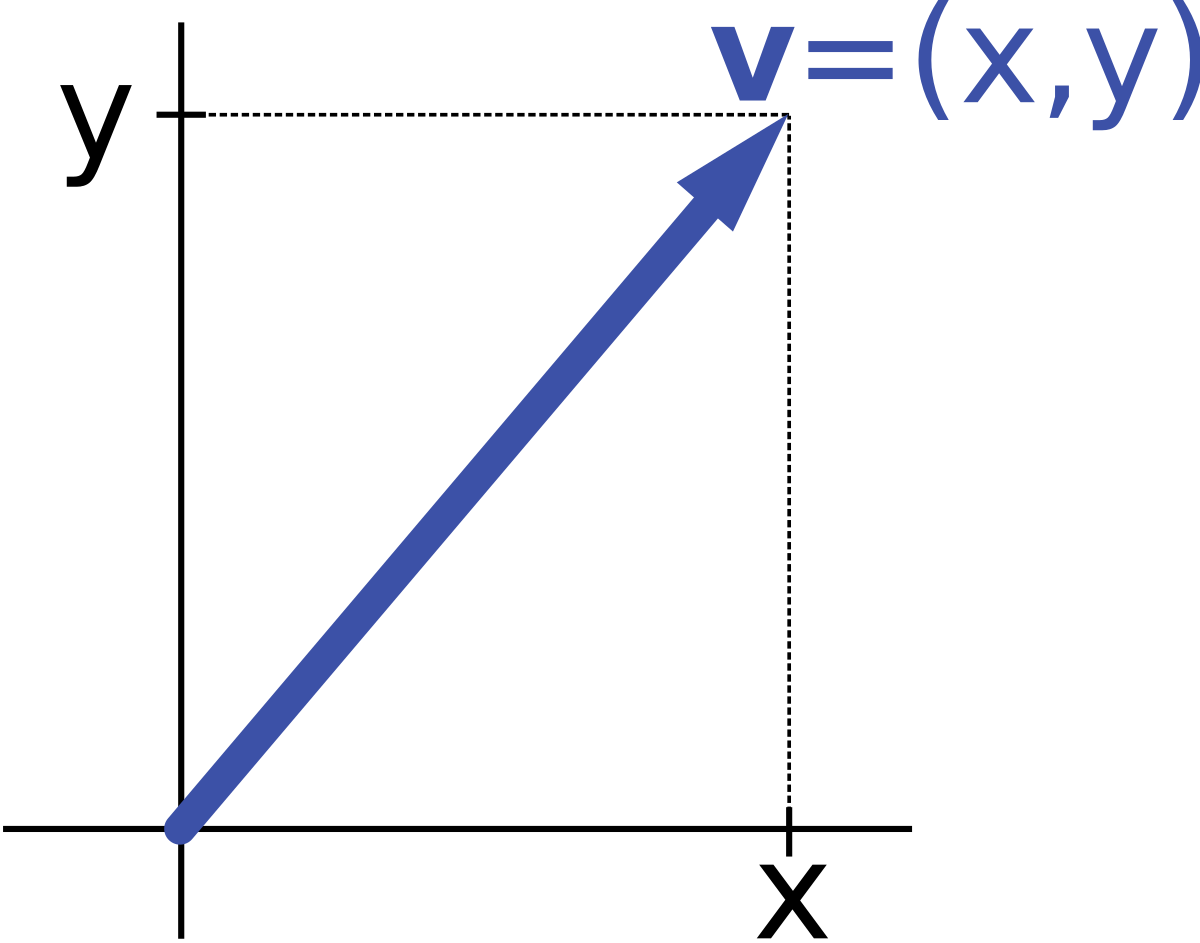
\includegraphics[width=5cm]{Vector_components.png}
\end{figure}


Python relies on a package called NumPy for linear algebra. Below is
code for importing the NumPy package and creating a simple vector.

    \begin{tcolorbox}[breakable, size=fbox, boxrule=1pt, pad at break*=1mm,colback=cellbackground, colframe=cellborder]
\prompt{In}{incolor}{ }{\boxspacing}
\begin{Verbatim}[commandchars=\\\{\}]
\PY{k+kn}{import} \PY{n+nn}{numpy} \PY{k}{as} \PY{n+nn}{np}
\PY{n}{v} \PY{o}{=} \PY{n}{np}\PY{o}{.}\PY{n}{array}\PY{p}{(}\PY{p}{[}\PY{l+m+mi}{1}\PY{p}{,}\PY{l+m+mi}{2}\PY{p}{,}\PY{l+m+mi}{3}\PY{p}{,}\PY{l+m+mi}{4}\PY{p}{,}\PY{l+m+mi}{5}\PY{p}{]}\PY{p}{)}
\PY{n+nb}{print}\PY{p}{(}\PY{n}{v}\PY{p}{)}
\end{Verbatim}
\end{tcolorbox}

    In Python indexing starts a zero, so the first number in our vector is
entry \(0\), the second is entry \(1\) and so on. To access specific
entries, we use square brackets

    \begin{tcolorbox}[breakable, size=fbox, boxrule=1pt, pad at break*=1mm,colback=cellbackground, colframe=cellborder]
\prompt{In}{incolor}{ }{\boxspacing}
\begin{Verbatim}[commandchars=\\\{\}]
\PY{n}{v}\PY{p}{[}\PY{l+m+mi}{2}\PY{p}{]}
\end{Verbatim}
\end{tcolorbox}

    \hypertarget{basic-operations}{%
\subsubsection{Basic operations}\label{basic-operations}}

\hypertarget{scalar-multiplication}{%
\paragraph{Scalar multiplication}\label{scalar-multiplication}}

A scalar is a single number, and scalar multiplication refers to
multiplying a vector by a single number. With scalar multiplication,
every entry is multiplied by this number.

    \begin{tcolorbox}[breakable, size=fbox, boxrule=1pt, pad at break*=1mm,colback=cellbackground, colframe=cellborder]
\prompt{In}{incolor}{ }{\boxspacing}
\begin{Verbatim}[commandchars=\\\{\}]
\PY{l+m+mi}{2}\PY{o}{*}\PY{n}{v}
\end{Verbatim}
\end{tcolorbox}

    \hypertarget{addition}{%
\paragraph{Addition}\label{addition}}

To add two vectors they must be the same length. The addition is
performed element-by-element, i.e.~the first element of vector one is
added to the first element of vector two, the second element of vector
one is added to the second element of vector two, and so on.

    \begin{tcolorbox}[breakable, size=fbox, boxrule=1pt, pad at break*=1mm,colback=cellbackground, colframe=cellborder]
\prompt{In}{incolor}{ }{\boxspacing}
\begin{Verbatim}[commandchars=\\\{\}]
\PY{n}{u} \PY{o}{=} \PY{n}{np}\PY{o}{.}\PY{n}{array}\PY{p}{(}\PY{p}{[}\PY{l+m+mi}{3}\PY{p}{,}\PY{l+m+mi}{7}\PY{p}{,}\PY{l+m+mi}{1}\PY{p}{,}\PY{l+m+mi}{6}\PY{p}{,}\PY{l+m+mi}{4}\PY{p}{]}\PY{p}{)}
\PY{n}{v}\PY{o}{+}\PY{n}{u}
\end{Verbatim}
\end{tcolorbox}

    \textbf{Exercise 2:} Add the vectors
\[a = \begin{bmatrix}5 \\ 1 \\ -9 \\ 3 \\ 7\end{bmatrix}, \qquad b = \begin{bmatrix}7 \\ 3 \\ 1 \\ -4 \\ 6\end{bmatrix}\]
by hand and then use Python to check your answer.

    \begin{tcolorbox}[breakable, size=fbox, boxrule=1pt, pad at break*=1mm,colback=cellbackground, colframe=cellborder]
\prompt{In}{incolor}{ }{\boxspacing}
\begin{Verbatim}[commandchars=\\\{\}]
\PY{n}{a} \PY{o}{=} \PY{n}{np}\PY{o}{.}\PY{n}{array}\PY{p}{(}\PY{p}{[}\PY{l+m+mi}{5}\PY{p}{,}\PY{l+m+mi}{1}\PY{p}{,}\PY{o}{\PYZhy{}}\PY{l+m+mi}{9}\PY{p}{,}\PY{l+m+mi}{3}\PY{p}{,}\PY{l+m+mi}{7}\PY{p}{]}\PY{p}{)}
\PY{n}{b} \PY{o}{=} \PY{n}{np}\PY{o}{.}\PY{n}{array}\PY{p}{(}\PY{p}{[}\PY{l+m+mi}{7}\PY{p}{,}\PY{l+m+mi}{3}\PY{p}{,}\PY{l+m+mi}{1}\PY{p}{,}\PY{o}{\PYZhy{}}\PY{l+m+mi}{4}\PY{p}{,}\PY{l+m+mi}{6}\PY{p}{]}\PY{p}{)}
\PY{n}{a}\PY{o}{+}\PY{n}{b}
\end{Verbatim}
\end{tcolorbox}

    \hypertarget{dot-product}{%
\paragraph{Dot product}\label{dot-product}}

The dot product of two vectors is computed by performing element-by
element multiplication and adding up all of the products,
\[u\cdot v = u_1v_1 + u_2v_2 + \dots +u_nv_n .\] As with adding two
vectors, the two vectors must be the same length. To compute the dot
product in Python we use the \texttt{dot()} function/method.

    \begin{tcolorbox}[breakable, size=fbox, boxrule=1pt, pad at break*=1mm,colback=cellbackground, colframe=cellborder]
\prompt{In}{incolor}{ }{\boxspacing}
\begin{Verbatim}[commandchars=\\\{\}]
\PY{n}{u}\PY{o}{.}\PY{n}{dot}\PY{p}{(}\PY{n}{v}\PY{p}{)}
\end{Verbatim}
\end{tcolorbox}

    \textbf{Note:} Using \texttt{u*v} will perform element-by-element
multiplication, but not sum up the products.

    \begin{tcolorbox}[breakable, size=fbox, boxrule=1pt, pad at break*=1mm,colback=cellbackground, colframe=cellborder]
\prompt{In}{incolor}{ }{\boxspacing}
\begin{Verbatim}[commandchars=\\\{\}]
\PY{n}{u}\PY{o}{*}\PY{n}{v}
\end{Verbatim}
\end{tcolorbox}

    \textbf{Exercise 3:} Compute the dot product of the vectors \(a\) and
\(b\) (given in Exercise 2) by hand. Then compute the dot product in
Python. Do the two answers match?

    \begin{tcolorbox}[breakable, size=fbox, boxrule=1pt, pad at break*=1mm,colback=cellbackground, colframe=cellborder]
\prompt{In}{incolor}{ }{\boxspacing}
\begin{Verbatim}[commandchars=\\\{\}]
\PY{n}{a}\PY{o}{.}\PY{n}{dot}\PY{p}{(}\PY{n}{b}\PY{p}{)}
\end{Verbatim}
\end{tcolorbox}

    \hypertarget{matrices}{%
\subsection{Matrices}\label{matrices}}

A matrix can be thought of as a collection of vectors of the same
length. An \(n\times m\) matrix is a rectangular array of numbers with
\(n\) rows and \(m\) columns. For example,
\[A=\begin{bmatrix}2 & 8 & 4 \\ 1 & 0 & 3 \\ 5 & 1 & 6 \\ 8 & 3& 5\end{bmatrix} \text{ is a } 4\times 3 \text{ matrix, while }B=\begin{bmatrix}1 & 2 \\ 3 & 4 \\ 5 & 6\end{bmatrix} \text{ is a } 3\times 2 \text{ matrix.}\]

In Python, matrices are create in a similar manner to vectors. We simply
give the \texttt{array} function a list of lists

    \begin{tcolorbox}[breakable, size=fbox, boxrule=1pt, pad at break*=1mm,colback=cellbackground, colframe=cellborder]
\prompt{In}{incolor}{ }{\boxspacing}
\begin{Verbatim}[commandchars=\\\{\}]
\PY{n}{A} \PY{o}{=} \PY{n}{np}\PY{o}{.}\PY{n}{array}\PY{p}{(}\PY{p}{[}\PY{p}{[}\PY{l+m+mi}{2}\PY{p}{,}\PY{l+m+mi}{8}\PY{p}{,}\PY{l+m+mi}{4}\PY{p}{]}\PY{p}{,}\PY{p}{[}\PY{l+m+mi}{1}\PY{p}{,}\PY{l+m+mi}{0}\PY{p}{,}\PY{l+m+mi}{3}\PY{p}{]}\PY{p}{,}\PY{p}{[}\PY{l+m+mi}{5}\PY{p}{,}\PY{l+m+mi}{1}\PY{p}{,}\PY{l+m+mi}{6}\PY{p}{]}\PY{p}{,}\PY{p}{[}\PY{l+m+mi}{8}\PY{p}{,}\PY{l+m+mi}{3}\PY{p}{,}\PY{l+m+mi}{5}\PY{p}{]}\PY{p}{]}\PY{p}{)}
\PY{n+nb}{print}\PY{p}{(}\PY{n}{A}\PY{p}{)}
\end{Verbatim}
\end{tcolorbox}

    \begin{tcolorbox}[breakable, size=fbox, boxrule=1pt, pad at break*=1mm,colback=cellbackground, colframe=cellborder]
\prompt{In}{incolor}{ }{\boxspacing}
\begin{Verbatim}[commandchars=\\\{\}]
\PY{n}{B} \PY{o}{=} \PY{n}{np}\PY{o}{.}\PY{n}{array}\PY{p}{(}\PY{p}{[}\PY{p}{[}\PY{l+m+mi}{1}\PY{p}{,}\PY{l+m+mi}{2}\PY{p}{]}\PY{p}{,}\PY{p}{[}\PY{l+m+mi}{3}\PY{p}{,}\PY{l+m+mi}{4}\PY{p}{]}\PY{p}{,}\PY{p}{[}\PY{l+m+mi}{5}\PY{p}{,}\PY{l+m+mi}{6}\PY{p}{]}\PY{p}{]}\PY{p}{)}
\PY{n+nb}{print}\PY{p}{(}\PY{n}{B}\PY{p}{)}
\end{Verbatim}
\end{tcolorbox}

    \begin{tcolorbox}[breakable, size=fbox, boxrule=1pt, pad at break*=1mm,colback=cellbackground, colframe=cellborder]
\prompt{In}{incolor}{ }{\boxspacing}
\begin{Verbatim}[commandchars=\\\{\}]
\PY{n}{A}\PY{p}{[}\PY{l+m+mi}{0}\PY{p}{,}\PY{l+m+mi}{1}\PY{p}{]}
\end{Verbatim}
\end{tcolorbox}

    \begin{tcolorbox}[breakable, size=fbox, boxrule=1pt, pad at break*=1mm,colback=cellbackground, colframe=cellborder]
\prompt{In}{incolor}{ }{\boxspacing}
\begin{Verbatim}[commandchars=\\\{\}]
\PY{n}{B}\PY{p}{[}\PY{l+m+mi}{2}\PY{p}{,}\PY{l+m+mi}{1}\PY{p}{]}
\end{Verbatim}
\end{tcolorbox}

    A common use of matrices is to digitally encode a picture. Imagine a
\(100\times 100\) pixel black and white image. Each pixel encodes the
level of brightness at the point, which is just a single number. Writing
down the brightness level at each pixel in a \(100\times 100\) grid
gives us a \(100\times 100\) matrix.

    \begin{tcolorbox}[breakable, size=fbox, boxrule=1pt, pad at break*=1mm,colback=cellbackground, colframe=cellborder]
\prompt{In}{incolor}{ }{\boxspacing}
\begin{Verbatim}[commandchars=\\\{\}]
\PY{n}{pixel\PYZus{}matrix} \PY{o}{=} \PY{n}{np}\PY{o}{.}\PY{n}{load}\PY{p}{(}\PY{l+s+s1}{\PYZsq{}}\PY{l+s+s1}{pixel\PYZus{}matrix.npy}\PY{l+s+s1}{\PYZsq{}}\PY{p}{)}
\PY{n+nb}{print}\PY{p}{(}\PY{n}{pixel\PYZus{}matrix}\PY{p}{)}
\PY{n+nb}{print}\PY{p}{(}\PY{n}{pixel\PYZus{}matrix}\PY{o}{.}\PY{n}{shape}\PY{p}{)}
\end{Verbatim}
\end{tcolorbox}

    Let's try plotting the matrix to see what it represents. We will first
need to load in Python's plotting library matplotlib:

    \begin{tcolorbox}[breakable, size=fbox, boxrule=1pt, pad at break*=1mm,colback=cellbackground, colframe=cellborder]
\prompt{In}{incolor}{ }{\boxspacing}
\begin{Verbatim}[commandchars=\\\{\}]
\PY{k+kn}{import} \PY{n+nn}{matplotlib}\PY{n+nn}{.}\PY{n+nn}{pyplot} \PY{k}{as} \PY{n+nn}{plt}
\end{Verbatim}
\end{tcolorbox}

    \begin{tcolorbox}[breakable, size=fbox, boxrule=1pt, pad at break*=1mm,colback=cellbackground, colframe=cellborder]
\prompt{In}{incolor}{ }{\boxspacing}
\begin{Verbatim}[commandchars=\\\{\}]
\PY{n}{plt}\PY{o}{.}\PY{n}{matshow}\PY{p}{(}\PY{n}{pixel\PYZus{}matrix}\PY{p}{,}\PY{n}{cmap}\PY{o}{=}\PY{l+s+s1}{\PYZsq{}}\PY{l+s+s1}{gray}\PY{l+s+s1}{\PYZsq{}}\PY{p}{)}
\PY{n}{plt}\PY{o}{.}\PY{n}{show}\PY{p}{(}\PY{p}{)}
\end{Verbatim}
\end{tcolorbox}

    \hypertarget{transpose}{%
\paragraph{Transpose}\label{transpose}}

The transpose of a matrix \(A\) is the matrix \(A^T\) with the rows and
columns of \(A\) swapped. For example
\[A=\begin{bmatrix}2 & 8 & 4 \\ 1 & 0 & 3 \\ 5 & 1 & 6 \\ 8 & 3& 5\end{bmatrix}, \qquad A^T = \begin{bmatrix}2 & 1 & 5 & 8  \\ 8 & 0 & 1 & 3 \\ 4 & 3 & 6 &5\end{bmatrix}.\]
The transpose of a \(n \times m\) matrix is an \(m \times n\) matrix.

    \begin{tcolorbox}[breakable, size=fbox, boxrule=1pt, pad at break*=1mm,colback=cellbackground, colframe=cellborder]
\prompt{In}{incolor}{ }{\boxspacing}
\begin{Verbatim}[commandchars=\\\{\}]
\PY{n}{np}\PY{o}{.}\PY{n}{transpose}\PY{p}{(}\PY{n}{B}\PY{p}{)}
\end{Verbatim}
\end{tcolorbox}

    The transpose of a column vector \(v\) is a row vector \(v^T\). If
\[v=\begin{bmatrix}x \\ y\\ z\end{bmatrix},\] then
\[v^T = \begin{bmatrix} x & y & z \end{bmatrix}.\] Note that Python
returns the same array for the transpose of a vector:

    \begin{tcolorbox}[breakable, size=fbox, boxrule=1pt, pad at break*=1mm,colback=cellbackground, colframe=cellborder]
\prompt{In}{incolor}{ }{\boxspacing}
\begin{Verbatim}[commandchars=\\\{\}]
\PY{n}{np}\PY{o}{.}\PY{n}{transpose}\PY{p}{(}\PY{n}{v}\PY{p}{)}
\end{Verbatim}
\end{tcolorbox}

    \hypertarget{basic-operations}{%
\subsubsection{Basic operations}\label{basic-operations}}

\hypertarget{scalar-multiplication}{%
\paragraph{Scalar multiplication}\label{scalar-multiplication}}

As with vectors, if we multiply a matrix by a scalar, we simply multiple
every entry in the matrix by that number.

    \begin{tcolorbox}[breakable, size=fbox, boxrule=1pt, pad at break*=1mm,colback=cellbackground, colframe=cellborder]
\prompt{In}{incolor}{ }{\boxspacing}
\begin{Verbatim}[commandchars=\\\{\}]
\PY{l+m+mi}{3}\PY{o}{*}\PY{n}{A}
\end{Verbatim}
\end{tcolorbox}

    \hypertarget{matrix-vector-multiplication}{%
\paragraph{Matrix-vector
multiplication}\label{matrix-vector-multiplication}}

We can multiple a \(n\times m\) matrix (\(A\)) by a \(m\)-dimensional
vector (\(x\)) and the result will be a \(n\)-dimensional vector. To
perform this multiplication we compute the dot product of each of the
rows of \(A\) with \(x\). The result is a vector with \(m\) entries,
where the first entry is dot product of the first row of \(A\) with
\(x\), the second entry is dot product of the second row of \(A\) with
\(x\), and so on.

\begin{figure}
  \centering
  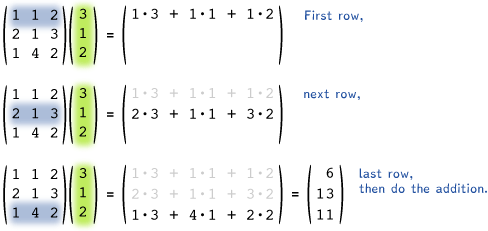
\includegraphics[width=10cm]{MatrixDefFigure7}
\end{figure}


    \begin{tcolorbox}[breakable, size=fbox, boxrule=1pt, pad at break*=1mm,colback=cellbackground, colframe=cellborder]
\prompt{In}{incolor}{ }{\boxspacing}
\begin{Verbatim}[commandchars=\\\{\}]
\PY{n}{x} \PY{o}{=} \PY{n}{np}\PY{o}{.}\PY{n}{array}\PY{p}{(}\PY{p}{[}\PY{p}{[}\PY{l+m+mi}{2}\PY{p}{]}\PY{p}{,}\PY{p}{[}\PY{l+m+mi}{1}\PY{p}{]}\PY{p}{]}\PY{p}{)}
\PY{n}{B}\PY{o}{.}\PY{n}{dot}\PY{p}{(}\PY{n}{x}\PY{p}{)}
\end{Verbatim}
\end{tcolorbox}

    \textbf{Note:} The order of multiplication matters! We cannot multiple a
\(m\)-dimensional vector by a \(n\times m\) matrix. The number of
columns in the first matrix/vector must be the same as the number of
rows in the second matrix/vector.

    \begin{tcolorbox}[breakable, size=fbox, boxrule=1pt, pad at break*=1mm,colback=cellbackground, colframe=cellborder]
\prompt{In}{incolor}{ }{\boxspacing}
\begin{Verbatim}[commandchars=\\\{\}]
\PY{n}{x}\PY{o}{.}\PY{n}{dot}\PY{p}{(}\PY{n}{B}\PY{p}{)}
\end{Verbatim}
\end{tcolorbox}

    \textbf{Exercise 4:} Compute the product \(Mu\), where
\[M = \begin{bmatrix}1 & 7 & 3 \\ 9 & 6 & 7\end{bmatrix}\quad \text{ and }\quad u = \begin{bmatrix} 2 \\ 9 \\ 6\end{bmatrix}\]by
hand and then use Python to check your answer.

    \begin{tcolorbox}[breakable, size=fbox, boxrule=1pt, pad at break*=1mm,colback=cellbackground, colframe=cellborder]
\prompt{In}{incolor}{ }{\boxspacing}
\begin{Verbatim}[commandchars=\\\{\}]
\PY{n}{M} \PY{o}{=} \PY{n}{np}\PY{o}{.}\PY{n}{array}\PY{p}{(}\PY{p}{[}\PY{p}{[}\PY{l+m+mi}{1}\PY{p}{,}\PY{l+m+mi}{7}\PY{p}{,}\PY{l+m+mi}{3}\PY{p}{]}\PY{p}{,}\PY{p}{[}\PY{l+m+mi}{9}\PY{p}{,}\PY{l+m+mi}{6}\PY{p}{,}\PY{l+m+mi}{7}\PY{p}{]}\PY{p}{]}\PY{p}{)}
\PY{n}{u} \PY{o}{=} \PY{n}{np}\PY{o}{.}\PY{n}{array}\PY{p}{(}\PY{p}{[}\PY{p}{[}\PY{l+m+mi}{2}\PY{p}{]}\PY{p}{,}\PY{p}{[}\PY{l+m+mi}{9}\PY{p}{]}\PY{p}{,} \PY{p}{[}\PY{l+m+mi}{6}\PY{p}{]}\PY{p}{]}\PY{p}{)}
\PY{n}{M}\PY{o}{.}\PY{n}{dot}\PY{p}{(}\PY{n}{u}\PY{p}{)}
\end{Verbatim}
\end{tcolorbox}

    \hypertarget{matrix-multiplication}{%
\paragraph{Matrix multiplication}\label{matrix-multiplication}}

Matrix multiplication is simply an extension of matrix-vector
multiplication. When multiplying two matrices we compute the dot product
of each row of matrix 1 with each column of matrix 2, and the resulting
matrix contains all of these dot products.

Lets take our matrices \(A\) and \(B\) from above and compute their
product:

    \begin{tcolorbox}[breakable, size=fbox, boxrule=1pt, pad at break*=1mm,colback=cellbackground, colframe=cellborder]
\prompt{In}{incolor}{ }{\boxspacing}
\begin{Verbatim}[commandchars=\\\{\}]
\PY{n}{A}\PY{o}{.}\PY{n}{dot}\PY{p}{(}\PY{n}{B}\PY{p}{)}
\end{Verbatim}
\end{tcolorbox}

    Multiplying a \(n\times m\) matrix by a \(m\times p\) matrix results in
a \(n\times p\) matrix.

\textbf{Note:} The number of columns in the first matrix must be the
same as the number of rows in the second matrix. Hence, the product
\(BA\) is not defined, as \(B\) has 2 columns and \(A\) has 4 rows.

    \textbf{Exercise 5:} Compute the product \(XY\), where
\[X = \begin{bmatrix} 5 & 1 \\ 6 & 3\end{bmatrix}\text{ and }Y = \begin{bmatrix} 3 & 7& 2 \\ 1 & 4 & 6\end{bmatrix}\]by
hand and then use Python to check your answer.

    \begin{tcolorbox}[breakable, size=fbox, boxrule=1pt, pad at break*=1mm,colback=cellbackground, colframe=cellborder]
\prompt{In}{incolor}{ }{\boxspacing}
\begin{Verbatim}[commandchars=\\\{\}]
\PY{n}{X} \PY{o}{=} \PY{n}{np}\PY{o}{.}\PY{n}{array}\PY{p}{(}\PY{p}{[}\PY{p}{[}\PY{l+m+mi}{5}\PY{p}{,}\PY{l+m+mi}{1}\PY{p}{]}\PY{p}{,}\PY{p}{[}\PY{l+m+mi}{6}\PY{p}{,}\PY{l+m+mi}{3}\PY{p}{]}\PY{p}{]}\PY{p}{)}
\PY{n}{Y} \PY{o}{=} \PY{n}{np}\PY{o}{.}\PY{n}{array}\PY{p}{(}\PY{p}{[}\PY{p}{[}\PY{l+m+mi}{3}\PY{p}{,}\PY{l+m+mi}{7}\PY{p}{,}\PY{l+m+mi}{2}\PY{p}{]}\PY{p}{,}\PY{p}{[}\PY{l+m+mi}{1}\PY{p}{,}\PY{l+m+mi}{4}\PY{p}{,}\PY{l+m+mi}{6}\PY{p}{]}\PY{p}{]}\PY{p}{)}
\PY{n}{X}\PY{o}{.}\PY{n}{dot}\PY{p}{(}\PY{n}{Y}\PY{p}{)}
\end{Verbatim}
\end{tcolorbox}

    \hypertarget{square-matrices}{%
\subsubsection{Square Matrices}\label{square-matrices}}

Square matrices have the same number of rows as columns. An important
square matrix is the \(n \times n\) identity matrix \(I_n\) which has
ones on the diagonal and zeros off the diagonal.

\[I_3 = \begin{bmatrix} 1 & 0 & 0 \\ 0 & 1 & 0 \\ 0 & 0 & 1\end{bmatrix}.\]

The identity matrix has the property that \(PI_n =P = I_nP\) for any
\(n \times n\) square matrix \(P\) and \(I_n v = v\) for any column
vector \(v\) of dimension \(n\).

For square matrices \(P\) and \(Q\) of the same dimension \(PQ\) and
\(QP\) both exist but \(PQ \neq QP\) in general.

\textbf{Exercise 6:} Compute and compare the products \(PQ\) and \(QP\)
where
\[P = \begin{bmatrix} 1 & 2 \\ 2 &2\end{bmatrix}\quad \text{ and }\quad Q  \begin{bmatrix} -2 & 1 \\ 4 & 6\end{bmatrix}.\]

    \begin{tcolorbox}[breakable, size=fbox, boxrule=1pt, pad at break*=1mm,colback=cellbackground, colframe=cellborder]
\prompt{In}{incolor}{ }{\boxspacing}
\begin{Verbatim}[commandchars=\\\{\}]
\PY{n}{P}\PY{o}{=}\PY{n}{np}\PY{o}{.}\PY{n}{array}\PY{p}{(}\PY{p}{[}\PY{p}{[}\PY{l+m+mi}{1}\PY{p}{,} \PY{l+m+mi}{2}\PY{p}{]}\PY{p}{,} \PY{p}{[}\PY{l+m+mi}{2}\PY{p}{,} \PY{l+m+mi}{2}\PY{p}{]}\PY{p}{]}\PY{p}{)}
\PY{n}{Q}\PY{o}{=}\PY{n}{np}\PY{o}{.}\PY{n}{array}\PY{p}{(}\PY{p}{[}\PY{p}{[}\PY{o}{\PYZhy{}}\PY{l+m+mi}{2}\PY{p}{,} \PY{l+m+mi}{1}\PY{p}{]}\PY{p}{,} \PY{p}{[}\PY{l+m+mi}{4}\PY{p}{,} \PY{l+m+mi}{6}\PY{p}{]}\PY{p}{]}\PY{p}{)}
\PY{n+nb}{print}\PY{p}{(}\PY{l+s+s2}{\PYZdq{}}\PY{l+s+s2}{PQ=}\PY{l+s+s2}{\PYZdq{}}\PY{p}{,}  \PY{n}{P}\PY{o}{.}\PY{n}{dot}\PY{p}{(}\PY{n}{Q}\PY{p}{)}\PY{p}{)}
\PY{n+nb}{print}\PY{p}{(}\PY{l+s+s1}{\PYZsq{}}\PY{l+s+s1}{QP=}\PY{l+s+s1}{\PYZsq{}}\PY{p}{,} \PY{n}{Q}\PY{o}{.}\PY{n}{dot}\PY{p}{(}\PY{n}{P}\PY{p}{)}\PY{p}{)}
\end{Verbatim}
\end{tcolorbox}

    \hypertarget{determinants}{%
\paragraph{Determinants}\label{determinants}}

The determinant of a square matrix, \(A\), is a scalar (number)
\(\det(A)\) that depends on the entries. For a \(2 \times 2\) matrix
\[A = \begin{bmatrix} a_{11} & a_{12}\\ a_{21}& a_{22} \end{bmatrix}, \quad \det (A) = a_{11}a_{22}- a_{12}a_{21}.\]
For a \(3 \times 3\) matrix
\[A = \begin{bmatrix} a_{11} & a_{12} & a_{13}\\ a_{21} & a_{22}& a_{23} \\ a_{31} & a_{32} & a_{33}\end{bmatrix},\]
\begin{align*} \det (A) &= a_{11} \det\left( \begin{bmatrix} a_{22} & a_{23} \\ a_{32}& a_{33} \end{bmatrix}\right)  - a_{12} \det\left( \begin{bmatrix} a_{21} & a_{23} \\ a_{31}& a_{33}  \end{bmatrix}\right) + a_{13} \det\left( \begin{bmatrix} a_{21} & a_{22} \\ a_{31}& a_{32} \end{bmatrix}\right) \\ & = a_{11}(a_{22}a_{33} -a_{23}a_{32}) - a_{12}(a_{21}a_{33} -a_{23}a_{31}) + a_{13}(a_{21}a_{32}-a_{22}a_{31}).\end{align*}

The form of the determinant of an \(n \times n\) matrix can be found on
\href{https://en.wikipedia.org/wiki/Determinant}{Wikipedia
(determinants)}. Python can compute determinants for you.

    \begin{tcolorbox}[breakable, size=fbox, boxrule=1pt, pad at break*=1mm,colback=cellbackground, colframe=cellborder]
\prompt{In}{incolor}{ }{\boxspacing}
\begin{Verbatim}[commandchars=\\\{\}]
\PY{n}{np}\PY{o}{.}\PY{n}{linalg}\PY{o}{.}\PY{n}{det}\PY{p}{(}\PY{n}{P}\PY{p}{)}
\end{Verbatim}
\end{tcolorbox}

    \begin{tcolorbox}[breakable, size=fbox, boxrule=1pt, pad at break*=1mm,colback=cellbackground, colframe=cellborder]
\prompt{In}{incolor}{ }{\boxspacing}
\begin{Verbatim}[commandchars=\\\{\}]
\PY{n}{Q}\PY{o}{=}\PY{n}{np}\PY{o}{.}\PY{n}{array}\PY{p}{(}\PY{p}{[}\PY{p}{[}\PY{o}{\PYZhy{}}\PY{l+m+mi}{2}\PY{p}{,} \PY{l+m+mi}{1}\PY{p}{,} \PY{l+m+mi}{3}\PY{p}{,} \PY{o}{\PYZhy{}}\PY{l+m+mi}{4}\PY{p}{]}\PY{p}{,} \PY{p}{[}\PY{l+m+mi}{4}\PY{p}{,} \PY{l+m+mi}{6}\PY{p}{,} \PY{l+m+mi}{3}\PY{p}{,} \PY{l+m+mi}{2}\PY{p}{]}\PY{p}{,} \PY{p}{[}\PY{l+m+mi}{1}\PY{p}{,} \PY{o}{\PYZhy{}}\PY{l+m+mi}{1}\PY{p}{,} \PY{l+m+mi}{0}\PY{p}{,} \PY{l+m+mi}{4}\PY{p}{]}\PY{p}{,} \PY{p}{[}\PY{l+m+mi}{0}\PY{p}{,} \PY{l+m+mi}{1}\PY{p}{,} \PY{l+m+mi}{5}\PY{p}{,} \PY{l+m+mi}{2}\PY{p}{]}\PY{p}{]}\PY{p}{)}
\PY{n+nb}{round}\PY{p}{(}\PY{n}{np}\PY{o}{.}\PY{n}{linalg}\PY{o}{.}\PY{n}{det}\PY{p}{(}\PY{n}{Q}\PY{p}{)}\PY{p}{)}
\end{Verbatim}
\end{tcolorbox}

    \hypertarget{inverses}{%
\paragraph{Inverses}\label{inverses}}

If an \(n \times n\) square matrix \(A\) has \(\det(A) \neq 0\) then
\(A\) has an inverse matrix \(A^{-1}\) satisfying
\(A A^{-1} = A^{-1} A = I_n\). If \(\det(A) =0\) then \(A\) is singular
and has no inverse. For a \(2 \times 2\) matrix \(A\), if
\(\det(A) \neq 0\) then
\[A = \begin{bmatrix} a_{11} & a_{12}\\ a_{21}& a_{22} \end{bmatrix}, \quad A^{-1} = \frac{1}{\det{A}} \begin{bmatrix} a_{22} & -a_{12} \\ -a_{21}& a_{11} \end{bmatrix}.\]

Suppose that \(A v = b\) for a given invertible square matrix \(A\) and
vector \(b\) and that the vector \(v\) is unknown. Then multiplying both
sides on the left by \(A^{-1}\) we have \[v = A^{-1} b.\]

There is a way to compute inverse matrices in higher dimensions by hand:
see \href{https://en.wikipedia.org/wiki/Invertible_matrix}{Wikipedia
(Invertible matrix)}, but it is tedious. Python can calculate inverse
matrices

    \begin{tcolorbox}[breakable, size=fbox, boxrule=1pt, pad at break*=1mm,colback=cellbackground, colframe=cellborder]
\prompt{In}{incolor}{ }{\boxspacing}
\begin{Verbatim}[commandchars=\\\{\}]
\PY{n}{np}\PY{o}{.}\PY{n}{linalg}\PY{o}{.}\PY{n}{inv}\PY{p}{(}\PY{n}{P}\PY{p}{)}
\end{Verbatim}
\end{tcolorbox}

    \begin{tcolorbox}[breakable, size=fbox, boxrule=1pt, pad at break*=1mm,colback=cellbackground, colframe=cellborder]
\prompt{In}{incolor}{ }{\boxspacing}
\begin{Verbatim}[commandchars=\\\{\}]
\PY{n}{np}\PY{o}{.}\PY{n}{linalg}\PY{o}{.}\PY{n}{inv}\PY{p}{(}\PY{n}{Q}\PY{p}{)}
\end{Verbatim}
\end{tcolorbox}

    \hypertarget{eigenvalues-and-eigenvectors}{%
\paragraph{Eigenvalues and
eigenvectors}\label{eigenvalues-and-eigenvectors}}

Let \(M\) be an \(n \times n\) square matrix. If \(Mv = \lambda v\) for
some nonzero vector \(v\) and scalar \(\lambda\) then we say that
\(\lambda\) is an eigenvalue of \(M\) with corresponding eigenvector
\(v\).

For example

\[\begin{bmatrix} 1 & 5 \\ 2 & 4\end{bmatrix}\begin{bmatrix} 1 \\ 1 \end{bmatrix}  = 6\begin{bmatrix} 1 \\ 1 \end{bmatrix}\]
therefore \(6\) is an eigenvalue of~the matrix with eigenvector
\(\begin{bmatrix} 1 & 1 \end{bmatrix}^T.\)

If \(M v = \lambda v\) then
\[ M v - \lambda v= 0 \qquad \Rightarrow \qquad ( M -\lambda I_n )v= 0.\]~
If we multiply on the left by \(( M -\lambda I_n )^{-1}\) then we see
that \(v=0\) which is excluded. Therefore we conclude
that~\(( M -\lambda I_n )^{-1}\) does not exist. That is,
\(( M -\lambda I_n )\) is singular so \(\det( M -\lambda I_n )= 0\).
Therefore the eigenvalues of \(M\) are the values \(\lambda\) such that
\(\det( M -\lambda I_n )= 0\) which can be used to compute the
eigenvalues as the roots of a polynomial of degree \(n\) called the
characteristic polynomial.

For example if \(M= \begin{bmatrix} 1 & 5 \\ 2 & 4\end{bmatrix}\) then
\begin{align*} \det(M- \lambda I_2) &= \det\left( \begin{bmatrix} 1-\lambda  & 5 \\ 2 & 4-\lambda \end{bmatrix}\right) \\ & = (1-\lambda)(4-\lambda) -10 \\ & = \lambda^2 -5\lambda -6 \\ & = (\lambda -6)(\lambda +1). \end{align*}
This is zero when \(\lambda =6\) or \(\lambda=-1\) so these are the
eigenvalues of \(M\)

\textbf{Exercise 7:} Calculate the eigenvalues of
\[M = \begin{bmatrix} 5 & 2 \\ 2 & 5\end{bmatrix}\] by hand and then
check your answer by running the code below.

    \begin{tcolorbox}[breakable, size=fbox, boxrule=1pt, pad at break*=1mm,colback=cellbackground, colframe=cellborder]
\prompt{In}{incolor}{ }{\boxspacing}
\begin{Verbatim}[commandchars=\\\{\}]
\PY{n}{M}\PY{o}{=}\PY{n}{np}\PY{o}{.}\PY{n}{array}\PY{p}{(}\PY{p}{[}\PY{p}{[}\PY{l+m+mi}{5}\PY{p}{,}\PY{l+m+mi}{2}\PY{p}{]}\PY{p}{,} \PY{p}{[}\PY{l+m+mi}{2}\PY{p}{,}\PY{l+m+mi}{5}\PY{p}{]}\PY{p}{]}\PY{p}{)}
\PY{n}{np}\PY{o}{.}\PY{n}{linalg}\PY{o}{.}\PY{n}{eig}\PY{p}{(}\PY{n}{M}\PY{p}{)}
\end{Verbatim}
\end{tcolorbox}

    The first array shows the eigenvalues and the corresponding eigenvectors
are the columns of the second array. Note that eigenvectors \(v\) can
also be computed by hand, but we won't do that here. See
\href{https://en.wikipedia.org/wiki/Eigenvalues_and_eigenvectors}{Wikipedia
(Eigenvalues and Eigenvectors)} for details.

    \hypertarget{solving-differential-equations-numerically}{%
\section{Solving differential equations
numerically}\label{solving-differential-equations-numerically}}

Now that we know how to store numbers in arrays and perform basic
manipulations on these arrays, we can develop tools for studying
differential equations.

We begin by looking at how to determine numerical estimates for
solutions to ordinary differential equations. See the Wikipedia page
\href{https://en.wikipedia.org/wiki/Numerical_methods_for_ordinary_differential_equations}{Numerical\_methods\_for\_ordinary\_differential\_equation}
for an overview of the different numerical methods for solving ODEs. We
will give a brief summary of a couple of the simplest or most commonly
used methods. In practice, you will likely use a built in ODE solver.

    \hypertarget{eulers-method}{%
\subsection{Euler's method}\label{eulers-method}}

Euler's method is the simplest numerical method for estimating the
solution of a differential equation. Similar to when we
\emph{discretised} the equation for unrestricted population growth and
asked what the population increase was each year, Euler's method takes
small time steps and computes the increase at each time step. The
smaller the time step is, the more accurate the solution.

To approximately solve a differential equation
\[\frac{{\rm d}y}{{\rm d} x}= f(x, y)\] with \(y(x_0)=y_0\) and step
size \(h\), approximate the value of \(y\) at \(x_1 = x_0 +h\) by
\(y_1 = y_0 + h f(x_0, y_0)\) where \(f(x_0, y_0)\) is the derivative of
\(y\) at \((x_0, y_0)\). Repeating this for further steps

\[y_{n+1} = y_n + h f(x_n,y_n)\] is the approximate value of
\(y(x_0 + nh)\).

\begin{figure}
  \centering
  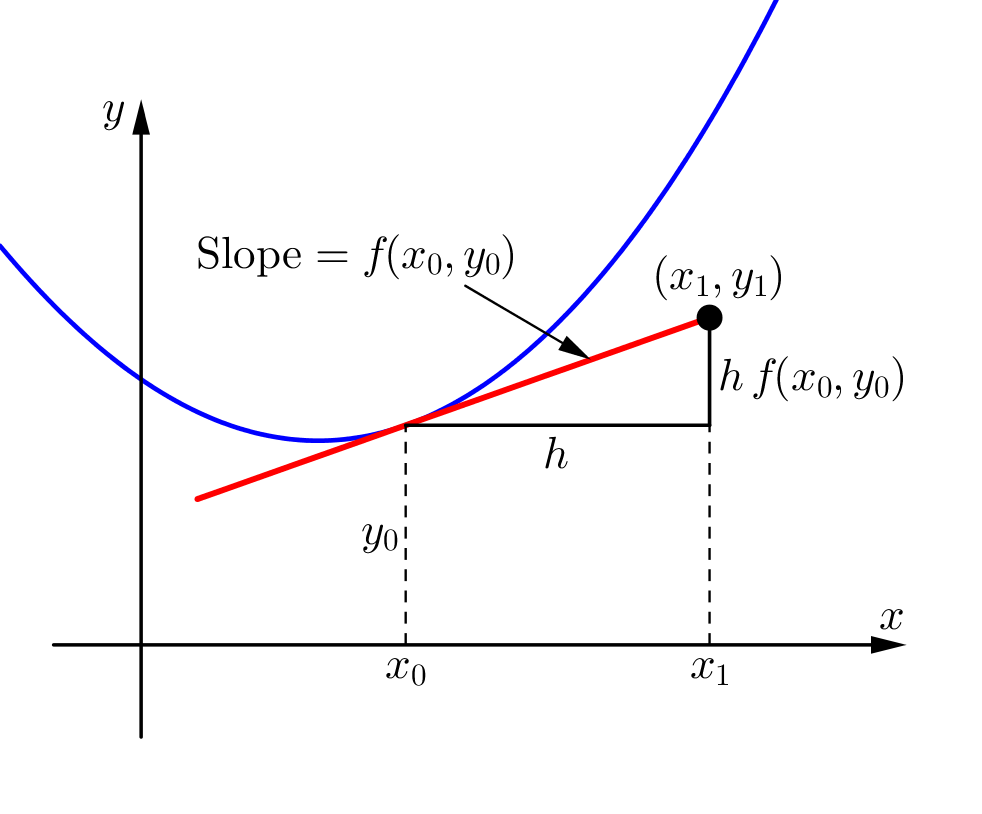
\includegraphics[width=7cm]{eulerdiagram}
\end{figure}

For the model of unrestricted population growth, the Euler method is
defined as \[N_{n+1} = N_n + \Delta t \times a N_n,\] where \(\Delta t\)
is the length of the time step we take.

The first thing we should do is define a function to represent the
right-hand side of our differential equation:

    \begin{tcolorbox}[breakable, size=fbox, boxrule=1pt, pad at break*=1mm,colback=cellbackground, colframe=cellborder]
\prompt{In}{incolor}{ }{\boxspacing}
\begin{Verbatim}[commandchars=\\\{\}]
\PY{k}{def} \PY{n+nf}{dNdt}\PY{p}{(}\PY{n}{a}\PY{p}{,}\PY{n}{x}\PY{p}{)}\PY{p}{:}
    \PY{k}{return} \PY{n}{a}\PY{o}{*}\PY{n}{x}
\end{Verbatim}
\end{tcolorbox}

    Next, we set up the Euler's method and cycle through our time points,
estimating the solution at each timepoint.

    \begin{tcolorbox}[breakable, size=fbox, boxrule=1pt, pad at break*=1mm,colback=cellbackground, colframe=cellborder]
\prompt{In}{incolor}{ }{\boxspacing}
\begin{Verbatim}[commandchars=\\\{\}]
\PY{n}{N0} \PY{o}{=} \PY{l+m+mi}{10000}
\PY{n}{a} \PY{o}{=} \PY{l+m+mf}{0.1}
\PY{n}{dt} \PY{o}{=} \PY{l+m+mi}{1}
\PY{n}{t\PYZus{}est} \PY{o}{=} \PY{n}{np}\PY{o}{.}\PY{n}{arange}\PY{p}{(}\PY{l+m+mi}{0}\PY{p}{,}\PY{l+m+mi}{25}\PY{o}{+}\PY{n}{dt}\PY{p}{,}\PY{n}{dt}\PY{p}{)}
\PY{n}{N\PYZus{}est} \PY{o}{=} \PY{n}{np}\PY{o}{.}\PY{n}{zeros}\PY{p}{(}\PY{n}{t\PYZus{}est}\PY{o}{.}\PY{n}{size}\PY{p}{)}
\PY{n}{N\PYZus{}est}\PY{p}{[}\PY{l+m+mi}{0}\PY{p}{]} \PY{o}{=} \PY{n}{N0}
\PY{k}{for} \PY{n}{j} \PY{o+ow}{in} \PY{n+nb}{range}\PY{p}{(}\PY{n+nb}{len}\PY{p}{(}\PY{n}{t\PYZus{}est}\PY{p}{)}\PY{o}{\PYZhy{}}\PY{l+m+mi}{1}\PY{p}{)}\PY{p}{:}
    \PY{n}{N\PYZus{}est}\PY{p}{[}\PY{n}{j}\PY{o}{+}\PY{l+m+mi}{1}\PY{p}{]} \PY{o}{=} \PY{n}{N\PYZus{}est}\PY{p}{[}\PY{n}{j}\PY{p}{]} \PY{o}{+} \PY{n}{dt}\PY{o}{*}\PY{n}{dNdt}\PY{p}{(}\PY{n}{a}\PY{p}{,}\PY{n}{N\PYZus{}est}\PY{p}{[}\PY{n}{j}\PY{p}{]}\PY{p}{)}


\PY{n+nb}{print}\PY{p}{(}\PY{n}{N\PYZus{}est}\PY{p}{)}
\end{Verbatim}
\end{tcolorbox}

    Now we plot the estimated solution and the exact solution on the same
graph.

    \begin{tcolorbox}[breakable, size=fbox, boxrule=1pt, pad at break*=1mm,colback=cellbackground, colframe=cellborder]
\prompt{In}{incolor}{ }{\boxspacing}
\begin{Verbatim}[commandchars=\\\{\}]
\PY{n}{plt}\PY{o}{.}\PY{n}{figure}\PY{p}{(}\PY{p}{)}
\PY{n}{plt}\PY{o}{.}\PY{n}{plot}\PY{p}{(}\PY{n}{t\PYZus{}est}\PY{p}{,}\PY{n}{N\PYZus{}est}\PY{p}{,}\PY{n}{label}\PY{o}{=}\PY{l+s+s1}{\PYZsq{}}\PY{l+s+s1}{Estimate}\PY{l+s+s1}{\PYZsq{}}\PY{p}{)}
\PY{n}{plt}\PY{o}{.}\PY{n}{plot}\PY{p}{(}\PY{n}{t}\PY{p}{,}\PY{n}{N}\PY{p}{,}\PY{n}{label}\PY{o}{=}\PY{l+s+s1}{\PYZsq{}}\PY{l+s+s1}{Exact}\PY{l+s+s1}{\PYZsq{}}\PY{p}{)}
\PY{n}{plt}\PY{o}{.}\PY{n}{xlabel}\PY{p}{(}\PY{l+s+s1}{\PYZsq{}}\PY{l+s+s1}{Time (years)}\PY{l+s+s1}{\PYZsq{}}\PY{p}{)}
\PY{n}{plt}\PY{o}{.}\PY{n}{ylabel}\PY{p}{(}\PY{l+s+s1}{\PYZsq{}}\PY{l+s+s1}{Population size}\PY{l+s+s1}{\PYZsq{}}\PY{p}{)}
\PY{n}{plt}\PY{o}{.}\PY{n}{axis}\PY{p}{(}\PY{p}{[}\PY{l+m+mi}{0}\PY{p}{,}\PY{l+m+mi}{25}\PY{p}{,}\PY{n}{N0}\PY{p}{,}\PY{l+m+mi}{121000}\PY{p}{]}\PY{p}{)}
\PY{n}{plt}\PY{o}{.}\PY{n}{legend}\PY{p}{(}\PY{p}{)}
\PY{n}{plt}\PY{o}{.}\PY{n}{show}\PY{p}{(}\PY{p}{)}
\end{Verbatim}
\end{tcolorbox}

    Examining the graph, we see that the estimated solution underestimates
the true solution and that it becomes more and more inaccurate as time
increases.

    \textbf{Exercise 8:} Change the step size \(\Delta t\) to 0.1 and run
the simulation again. What do you observe?

    \begin{tcolorbox}[breakable, size=fbox, boxrule=1pt, pad at break*=1mm,colback=cellbackground, colframe=cellborder]
\prompt{In}{incolor}{ }{\boxspacing}
\begin{Verbatim}[commandchars=\\\{\}]
\PY{n}{dt} \PY{o}{=} \PY{l+m+mf}{0.1}
\PY{n}{t\PYZus{}est2} \PY{o}{=} \PY{n}{np}\PY{o}{.}\PY{n}{arange}\PY{p}{(}\PY{l+m+mi}{0}\PY{p}{,}\PY{l+m+mi}{25}\PY{o}{+}\PY{n}{dt}\PY{p}{,}\PY{n}{dt}\PY{p}{)}
\PY{n}{N\PYZus{}est2} \PY{o}{=} \PY{n}{np}\PY{o}{.}\PY{n}{zeros}\PY{p}{(}\PY{n}{t\PYZus{}est2}\PY{o}{.}\PY{n}{size}\PY{p}{)}
\PY{n}{N\PYZus{}est2}\PY{p}{[}\PY{l+m+mi}{0}\PY{p}{]} \PY{o}{=} \PY{n}{N0}
\PY{k}{for} \PY{n}{j} \PY{o+ow}{in} \PY{n+nb}{range}\PY{p}{(}\PY{n+nb}{len}\PY{p}{(}\PY{n}{t\PYZus{}est2}\PY{p}{)}\PY{o}{\PYZhy{}}\PY{l+m+mi}{1}\PY{p}{)}\PY{p}{:}
    \PY{n}{N\PYZus{}est2}\PY{p}{[}\PY{n}{j}\PY{o}{+}\PY{l+m+mi}{1}\PY{p}{]} \PY{o}{=} \PY{n}{N\PYZus{}est2}\PY{p}{[}\PY{n}{j}\PY{p}{]} \PY{o}{+} \PY{n}{dt}\PY{o}{*}\PY{n}{dNdt}\PY{p}{(}\PY{n}{a}\PY{p}{,}\PY{n}{N\PYZus{}est2}\PY{p}{[}\PY{n}{j}\PY{p}{]}\PY{p}{)}

\PY{n}{plt}\PY{o}{.}\PY{n}{figure}\PY{p}{(}\PY{p}{)}
\PY{n}{plt}\PY{o}{.}\PY{n}{plot}\PY{p}{(}\PY{n}{t\PYZus{}est2}\PY{p}{,}\PY{n}{N\PYZus{}est2}\PY{p}{,}\PY{n}{label}\PY{o}{=}\PY{l+s+s1}{\PYZsq{}}\PY{l+s+s1}{Estimate}\PY{l+s+s1}{\PYZsq{}}\PY{p}{)}
\PY{n}{plt}\PY{o}{.}\PY{n}{plot}\PY{p}{(}\PY{n}{t}\PY{p}{,}\PY{n}{N}\PY{p}{,}\PY{n}{label}\PY{o}{=}\PY{l+s+s1}{\PYZsq{}}\PY{l+s+s1}{Exact}\PY{l+s+s1}{\PYZsq{}}\PY{p}{)}
\PY{n}{plt}\PY{o}{.}\PY{n}{xlabel}\PY{p}{(}\PY{l+s+s1}{\PYZsq{}}\PY{l+s+s1}{Time (years)}\PY{l+s+s1}{\PYZsq{}}\PY{p}{)}
\PY{n}{plt}\PY{o}{.}\PY{n}{ylabel}\PY{p}{(}\PY{l+s+s1}{\PYZsq{}}\PY{l+s+s1}{Population size}\PY{l+s+s1}{\PYZsq{}}\PY{p}{)}
\PY{n}{plt}\PY{o}{.}\PY{n}{axis}\PY{p}{(}\PY{p}{[}\PY{l+m+mi}{0}\PY{p}{,}\PY{l+m+mi}{25}\PY{p}{,}\PY{n}{N0}\PY{p}{,}\PY{l+m+mi}{121000}\PY{p}{]}\PY{p}{)}
\PY{n}{plt}\PY{o}{.}\PY{n}{legend}\PY{p}{(}\PY{p}{)}
\PY{n}{plt}\PY{o}{.}\PY{n}{show}\PY{p}{(}\PY{p}{)}
\end{Verbatim}
\end{tcolorbox}

    \hypertarget{runge-kutta-method}{%
\subsection{Runge-Kutta method}\label{runge-kutta-method}}

We can improve the accuracy of our numerical solver by including higher
order term. However, higher order methods require more calculations and
function evaluations, and as such, will take longer to run. In practice,
a good balance is achieved by the fourth order Runge--Kutta method.
Instead of simply using our current population size to estimate, say
next years population, we use estimates throughout the time interval
(the year) to determine our estimate. The solution at each time point is
computed as follows:
\[x_{n+1} = x_n + \frac{1}{6}\left(k_1+2k_2+2k_3+k_4\right)\] where
\begin{align*}k_1&=\Delta t f(x_n) \\
k_2&=\Delta t f(x_n+\tfrac{1}{2}k_1) \\
k_3&=\Delta t f(x_n+\tfrac{1}{2}k_2) \\
k_4&=\Delta t f(x_n+k_3) \end{align*}

See
\href{https://www.haroldserrano.com/blog/visualizing-the-runge-kutta-method}{Harold
Serrano's blog post} for a nice visualisation of the Runge-Kutta method.

As we did for Euler's method, we set up the Runge-Kutta method and
iterate over time to compute the estimated solution.

    \begin{tcolorbox}[breakable, size=fbox, boxrule=1pt, pad at break*=1mm,colback=cellbackground, colframe=cellborder]
\prompt{In}{incolor}{ }{\boxspacing}
\begin{Verbatim}[commandchars=\\\{\}]
\PY{n}{dt} \PY{o}{=} \PY{l+m+mi}{1}
\PY{n}{t\PYZus{}RK} \PY{o}{=} \PY{n}{np}\PY{o}{.}\PY{n}{arange}\PY{p}{(}\PY{l+m+mi}{0}\PY{p}{,}\PY{l+m+mi}{25}\PY{o}{+}\PY{n}{dt}\PY{p}{,}\PY{n}{dt}\PY{p}{)}
\PY{n}{N\PYZus{}RK} \PY{o}{=} \PY{n}{np}\PY{o}{.}\PY{n}{zeros}\PY{p}{(}\PY{n}{t\PYZus{}RK}\PY{o}{.}\PY{n}{size}\PY{p}{)}
\PY{n}{N\PYZus{}RK}\PY{p}{[}\PY{l+m+mi}{0}\PY{p}{]} \PY{o}{=} \PY{n}{N0}
\PY{k}{for} \PY{n}{n} \PY{o+ow}{in} \PY{n+nb}{range}\PY{p}{(}\PY{n+nb}{len}\PY{p}{(}\PY{n}{t\PYZus{}RK}\PY{p}{)}\PY{o}{\PYZhy{}}\PY{l+m+mi}{1}\PY{p}{)}\PY{p}{:}
    \PY{n}{k1} \PY{o}{=} \PY{n}{dt}\PY{o}{*}\PY{n}{dNdt}\PY{p}{(}\PY{n}{a}\PY{p}{,}\PY{n}{N\PYZus{}RK}\PY{p}{[}\PY{n}{n}\PY{p}{]}\PY{p}{)}
    \PY{n}{k2} \PY{o}{=} \PY{n}{dt}\PY{o}{*}\PY{n}{dNdt}\PY{p}{(}\PY{n}{a}\PY{p}{,}\PY{n}{N\PYZus{}RK}\PY{p}{[}\PY{n}{n}\PY{p}{]}\PY{o}{+}\PY{l+m+mf}{0.5}\PY{o}{*}\PY{n}{k1}\PY{p}{)}
    \PY{n}{k3} \PY{o}{=} \PY{n}{dt}\PY{o}{*}\PY{n}{dNdt}\PY{p}{(}\PY{n}{a}\PY{p}{,}\PY{n}{N\PYZus{}RK}\PY{p}{[}\PY{n}{n}\PY{p}{]}\PY{o}{+}\PY{l+m+mf}{0.5}\PY{o}{*}\PY{n}{k2}\PY{p}{)}
    \PY{n}{k4} \PY{o}{=} \PY{n}{dt}\PY{o}{*}\PY{n}{dNdt}\PY{p}{(}\PY{n}{a}\PY{p}{,}\PY{n}{N\PYZus{}RK}\PY{p}{[}\PY{n}{n}\PY{p}{]}\PY{o}{+}\PY{n}{k3}\PY{p}{)}
    \PY{n}{N\PYZus{}RK}\PY{p}{[}\PY{n}{n}\PY{o}{+}\PY{l+m+mi}{1}\PY{p}{]} \PY{o}{=} \PY{n}{N\PYZus{}RK}\PY{p}{[}\PY{n}{n}\PY{p}{]} \PY{o}{+} \PY{p}{(}\PY{n}{k1} \PY{o}{+} \PY{l+m+mi}{2}\PY{o}{*}\PY{n}{k2} \PY{o}{+} \PY{l+m+mi}{2}\PY{o}{*}\PY{n}{k3} \PY{o}{+} \PY{n}{k4}\PY{p}{)}\PY{o}{/}\PY{l+m+mi}{6}
\end{Verbatim}
\end{tcolorbox}

    Now plotting the exact solutions and the two estimated solutions.

    \begin{tcolorbox}[breakable, size=fbox, boxrule=1pt, pad at break*=1mm,colback=cellbackground, colframe=cellborder]
\prompt{In}{incolor}{ }{\boxspacing}
\begin{Verbatim}[commandchars=\\\{\}]
\PY{n}{plt}\PY{o}{.}\PY{n}{figure}\PY{p}{(}\PY{p}{)}
\PY{n}{plt}\PY{o}{.}\PY{n}{plot}\PY{p}{(}\PY{n}{t}\PY{p}{,}\PY{n}{N}\PY{p}{,}\PY{n}{label}\PY{o}{=}\PY{l+s+s1}{\PYZsq{}}\PY{l+s+s1}{Exact}\PY{l+s+s1}{\PYZsq{}}\PY{p}{)}
\PY{n}{plt}\PY{o}{.}\PY{n}{plot}\PY{p}{(}\PY{n}{t\PYZus{}est}\PY{p}{,}\PY{n}{N\PYZus{}est}\PY{p}{,}\PY{n}{label}\PY{o}{=}\PY{l+s+s1}{\PYZsq{}}\PY{l+s+s1}{Euler}\PY{l+s+s1}{\PYZsq{}}\PY{p}{)}
\PY{n}{plt}\PY{o}{.}\PY{n}{plot}\PY{p}{(}\PY{n}{t\PYZus{}RK}\PY{p}{,}\PY{n}{N\PYZus{}RK}\PY{p}{,}\PY{n}{label}\PY{o}{=}\PY{l+s+s1}{\PYZsq{}}\PY{l+s+s1}{Runge Kutta}\PY{l+s+s1}{\PYZsq{}}\PY{p}{)}

\PY{n}{plt}\PY{o}{.}\PY{n}{xlabel}\PY{p}{(}\PY{l+s+s1}{\PYZsq{}}\PY{l+s+s1}{Time (years)}\PY{l+s+s1}{\PYZsq{}}\PY{p}{)}
\PY{n}{plt}\PY{o}{.}\PY{n}{ylabel}\PY{p}{(}\PY{l+s+s1}{\PYZsq{}}\PY{l+s+s1}{Population size}\PY{l+s+s1}{\PYZsq{}}\PY{p}{)}
\PY{n}{plt}\PY{o}{.}\PY{n}{legend}\PY{p}{(}\PY{p}{)}
\PY{n}{plt}\PY{o}{.}\PY{n}{show}\PY{p}{(}\PY{p}{)}
\end{Verbatim}
\end{tcolorbox}

    Looking at the plot, we see that if we use the same time step for both
the Euler method and the Runge-Kutta method, the Runge-Kutta method
significantly outperforms the Euler method.

    \hypertarget{built-in-ode-solvers}{%
\subsection{Built-in ODE solvers}\label{built-in-ode-solvers}}

In practice, we usually rely on built-in ODE solvers. They are tried and
tested functions that will solve a system of ODEs to a high degree of
accuracy. These functions will typically be more efficient that one you
write yourself.

\href{https://docs.scipy.org/doc/scipy/reference/integrate.html}{Scipy's
integrate module} contains an array of functions for numerical calculus
(numerical differentiation, numerical integration, ODE solvers etc.).
You can find a list of all of the ODE solvers included in the integrate
module
\href{https://docs.scipy.org/doc/scipy/reference/integrate.html\#solving-initial-value-problems-for-ode-systems}{here}.

We will focus on the
\href{https://docs.scipy.org/doc/scipy/reference/generated/scipy.integrate.solve_ivp.html\#scipy.integrate.solve_ivp}{solve\_ivp
function} as it allows us choose from a list of integration methods. The
default is the 4th order Runge-Kutta method, with an adaptive step size
(updates the step size throughout the simulation, balancing accuracy and
efficiency).

    \begin{tcolorbox}[breakable, size=fbox, boxrule=1pt, pad at break*=1mm,colback=cellbackground, colframe=cellborder]
\prompt{In}{incolor}{ }{\boxspacing}
\begin{Verbatim}[commandchars=\\\{\}]
\PY{k+kn}{from} \PY{n+nn}{scipy}\PY{n+nn}{.}\PY{n+nn}{integrate} \PY{k+kn}{import} \PY{n}{solve\PYZus{}ivp}
\end{Verbatim}
\end{tcolorbox}

    To use any of the ODE solvers from Scipy's integrate module we must
define a function where the first two input arguments are time \(t\) and
the variable/list of variables \(x\), in that order. The system
parameter can then be defined as additional input arguments

    \begin{tcolorbox}[breakable, size=fbox, boxrule=1pt, pad at break*=1mm,colback=cellbackground, colframe=cellborder]
\prompt{In}{incolor}{ }{\boxspacing}
\begin{Verbatim}[commandchars=\\\{\}]
\PY{k}{def} \PY{n+nf}{dNdt\PYZus{}ivp}\PY{p}{(}\PY{n}{t}\PY{p}{,}\PY{n}{N}\PY{p}{,}\PY{n}{a}\PY{p}{)}\PY{p}{:}
    \PY{k}{return} \PY{n}{a}\PY{o}{*}\PY{n}{N}
\end{Verbatim}
\end{tcolorbox}

    The syntax for solve\_ivp is
\texttt{(function\ name,\ {[}t\ start,\ t\ end{]},\ initial\ conditions,\ args)}.
You can include additional arguments to specify the integration method,
the tolerance, step size, etc. Read the
\href{https://docs.scipy.org/doc/scipy/reference/generated/scipy.integrate.solve_ivp.html}{function
documentation} for more details.

    \begin{tcolorbox}[breakable, size=fbox, boxrule=1pt, pad at break*=1mm,colback=cellbackground, colframe=cellborder]
\prompt{In}{incolor}{ }{\boxspacing}
\begin{Verbatim}[commandchars=\\\{\}]
\PY{n}{sol} \PY{o}{=} \PY{n}{solve\PYZus{}ivp}\PY{p}{(}\PY{n}{dNdt\PYZus{}ivp}\PY{p}{,} \PY{p}{[}\PY{l+m+mi}{0}\PY{p}{,} \PY{l+m+mi}{25}\PY{p}{]}\PY{p}{,} \PY{p}{[}\PY{n}{N0}\PY{p}{]}\PY{p}{,} \PY{n}{args}\PY{o}{=}\PY{p}{(}\PY{n}{a}\PY{p}{,}\PY{p}{)}\PY{p}{,} \PY{n}{dense\PYZus{}output}\PY{o}{=}\PY{k+kc}{True}\PY{p}{)}
\end{Verbatim}
\end{tcolorbox}

    We can evaluate the solution for an array of time points and plot the
solution:

    \begin{tcolorbox}[breakable, size=fbox, boxrule=1pt, pad at break*=1mm,colback=cellbackground, colframe=cellborder]
\prompt{In}{incolor}{ }{\boxspacing}
\begin{Verbatim}[commandchars=\\\{\}]
\PY{n}{t\PYZus{}ivp} \PY{o}{=} \PY{n}{np}\PY{o}{.}\PY{n}{linspace}\PY{p}{(}\PY{l+m+mi}{0}\PY{p}{,} \PY{l+m+mi}{25}\PY{p}{,} \PY{l+m+mi}{501}\PY{p}{)}
\PY{n}{N\PYZus{}ivp} \PY{o}{=} \PY{n}{sol}\PY{o}{.}\PY{n}{sol}\PY{p}{(}\PY{n}{t\PYZus{}ivp}\PY{p}{)}

\PY{n}{plt}\PY{o}{.}\PY{n}{figure}\PY{p}{(}\PY{n}{figsize}\PY{o}{=}\PY{p}{(}\PY{l+m+mi}{12}\PY{p}{,}\PY{l+m+mi}{6}\PY{p}{)}\PY{p}{)}
\PY{n}{plt}\PY{o}{.}\PY{n}{subplot}\PY{p}{(}\PY{l+m+mi}{1}\PY{p}{,}\PY{l+m+mi}{2}\PY{p}{,}\PY{l+m+mi}{1}\PY{p}{)}
\PY{n}{plt}\PY{o}{.}\PY{n}{plot}\PY{p}{(}\PY{n}{t}\PY{p}{,}\PY{n}{N}\PY{p}{,}\PY{n}{label}\PY{o}{=}\PY{l+s+s1}{\PYZsq{}}\PY{l+s+s1}{Exact}\PY{l+s+s1}{\PYZsq{}}\PY{p}{)}
\PY{n}{plt}\PY{o}{.}\PY{n}{plot}\PY{p}{(}\PY{n}{t\PYZus{}est}\PY{p}{,}\PY{n}{N\PYZus{}est}\PY{p}{,}\PY{n}{label}\PY{o}{=}\PY{l+s+s1}{\PYZsq{}}\PY{l+s+s1}{Euler}\PY{l+s+s1}{\PYZsq{}}\PY{p}{)}
\PY{n}{plt}\PY{o}{.}\PY{n}{plot}\PY{p}{(}\PY{n}{t\PYZus{}RK}\PY{p}{,}\PY{n}{N\PYZus{}RK}\PY{p}{,}\PY{n}{label}\PY{o}{=}\PY{l+s+s1}{\PYZsq{}}\PY{l+s+s1}{Runge Kutta}\PY{l+s+s1}{\PYZsq{}}\PY{p}{)}
\PY{n}{plt}\PY{o}{.}\PY{n}{plot}\PY{p}{(}\PY{n}{t\PYZus{}ivp}\PY{p}{,}\PY{n}{N\PYZus{}ivp}\PY{p}{[}\PY{l+m+mi}{0}\PY{p}{]}\PY{p}{,}\PY{n}{label}\PY{o}{=}\PY{l+s+s1}{\PYZsq{}}\PY{l+s+s1}{Built\PYZhy{}in}\PY{l+s+s1}{\PYZsq{}}\PY{p}{)}

\PY{n}{plt}\PY{o}{.}\PY{n}{xlabel}\PY{p}{(}\PY{l+s+s1}{\PYZsq{}}\PY{l+s+s1}{Time (years)}\PY{l+s+s1}{\PYZsq{}}\PY{p}{)}
\PY{n}{plt}\PY{o}{.}\PY{n}{ylabel}\PY{p}{(}\PY{l+s+s1}{\PYZsq{}}\PY{l+s+s1}{Population size}\PY{l+s+s1}{\PYZsq{}}\PY{p}{)}
\PY{n}{plt}\PY{o}{.}\PY{n}{legend}\PY{p}{(}\PY{p}{)}


\PY{n}{plt}\PY{o}{.}\PY{n}{subplot}\PY{p}{(}\PY{l+m+mi}{1}\PY{p}{,}\PY{l+m+mi}{2}\PY{p}{,}\PY{l+m+mi}{2}\PY{p}{)}
\PY{n}{plt}\PY{o}{.}\PY{n}{plot}\PY{p}{(}\PY{n}{t}\PY{p}{,}\PY{n}{N}\PY{p}{,}\PY{n}{label}\PY{o}{=}\PY{l+s+s1}{\PYZsq{}}\PY{l+s+s1}{Exact}\PY{l+s+s1}{\PYZsq{}}\PY{p}{)}
\PY{n}{plt}\PY{o}{.}\PY{n}{plot}\PY{p}{(}\PY{n}{t\PYZus{}RK}\PY{p}{,}\PY{n}{N\PYZus{}RK}\PY{p}{,}\PY{n}{label}\PY{o}{=}\PY{l+s+s1}{\PYZsq{}}\PY{l+s+s1}{Runge Kutta}\PY{l+s+s1}{\PYZsq{}}\PY{p}{)}
\PY{n}{plt}\PY{o}{.}\PY{n}{plot}\PY{p}{(}\PY{n}{t\PYZus{}ivp}\PY{p}{,}\PY{n}{N\PYZus{}ivp}\PY{p}{[}\PY{l+m+mi}{0}\PY{p}{]}\PY{p}{,}\PY{n}{label}\PY{o}{=}\PY{l+s+s1}{\PYZsq{}}\PY{l+s+s1}{Built\PYZhy{}in}\PY{l+s+s1}{\PYZsq{}}\PY{p}{)}
\PY{n}{plt}\PY{o}{.}\PY{n}{legend}\PY{p}{(}\PY{p}{)}

\PY{n}{plt}\PY{o}{.}\PY{n}{xlabel}\PY{p}{(}\PY{l+s+s1}{\PYZsq{}}\PY{l+s+s1}{Time (years)}\PY{l+s+s1}{\PYZsq{}}\PY{p}{)}
\PY{n}{plt}\PY{o}{.}\PY{n}{axis}\PY{p}{(}\PY{p}{[}\PY{l+m+mf}{24.8}\PY{p}{,}\PY{l+m+mi}{25}\PY{p}{,}\PY{l+m+mi}{119000}\PY{p}{,}\PY{l+m+mi}{122000}\PY{p}{]}\PY{p}{)}
\PY{n}{plt}\PY{o}{.}\PY{n}{show}\PY{p}{(}\PY{p}{)}
\end{Verbatim}
\end{tcolorbox}

    \textbf{Note:} we need to include \texttt{dense\_output=True} as an
additional argument to evaluate the solution on a dense mesh.

    \textbf{Exercise 9:} Consider a system described by the following ODE
\[\dot{x}=x(1-x).\] Define a function \texttt{dxdt} for the right-hand
side of this expression, using the notation specied above (first two
arguments must be \(t\) and \(x\)). Then use the \texttt{solve\_ivp}
function to estimate the solution \(x(t)\) on the interval
\(0 \le t \le 10\) and initial value \(x(0)=0.5\).

    \begin{tcolorbox}[breakable, size=fbox, boxrule=1pt, pad at break*=1mm,colback=cellbackground, colframe=cellborder]
\prompt{In}{incolor}{ }{\boxspacing}
\begin{Verbatim}[commandchars=\\\{\}]

\end{Verbatim}
\end{tcolorbox}

    \hypertarget{simulating-the-hodgkin-huxley-hh-model}{%
\subsection{Simulating the Hodgkin-Huxley (HH)
model}\label{simulating-the-hodgkin-huxley-hh-model}}

Now that we understand what ODEs are and how we can simulate them
computationally, we return to the model of Hodgkin and Huxley:
\begin{align*}&C\frac{{\rm d}V}{{\rm d}t} = I - \overline{g}_{\text{Na}} m^3h (V-V_{\text{Na}}) - \overline{g}_{\text{K}} n^4 (V-V_{\text{K}}) - \overline{g}_l (V-V_l) \\
&\frac{{\rm d}n}{{\rm d}t} = \alpha_n(V)(1-n)-\beta_n(V)n \\
&\frac{{\rm d}m}{{\rm d}t} = \alpha_m(V)(1-m)-\beta_m(V)m \\
&\frac{{\rm d}h}{{\rm d}t} = \alpha_h(V)(1-h)-\beta_h(V)h\end{align*}

\begin{quote}
These are same as the form of the equations earlier with
\(X_\infty(V) = \alpha_X(V) \tau_X(V)\),
\(\tau_X(V) = (\alpha_X(V) + \beta_X(V))^{-1}\) for
\(X \in \{ n, m, h\}\).
\end{quote}

    \hypertarget{aside-what-do-all-of-the-terms-in-the-equations-mean-and-where-do-they-come-from}{%
\subsubsection{Aside: What do all of the terms in the equations mean and
where do they come
from?}\label{aside-what-do-all-of-the-terms-in-the-equations-mean-and-where-do-they-come-from}}

Differences in ion concentrations inside and outside of the neuron
create an electrical potential difference called the membrane potential
(\(V(t)\)). Here the neuron is considered to have the same membrane
potential \(V(t)\) everywhere across the cell (isopotential). The
constant that describes the relationship between the voltage and charge
\(Q(t)\) that builds up is called the capacitance (\(C\)).
Differentiating the identity \(Q=CV\),
\(C \frac{{\rm d}V}{{\rm d} t} = \frac{{\rm d}Q}{{\rm d} t} = I(t)\)
where \(I(t)\) is current. We then have, by conservation of electric
charge, \[ C  \frac{{\rm d}V}{{\rm d} t} = - I_{\text{ion}} + I,\] where
\(I\) is applied current and \(I_{\text{ion}}\) is the sum of individual
ionic currents. HH considers three currents (Na\(^+\), K\(^+\) and a
leak current). Each ionic current has a reversal potential (the value of
\(V\) at which there is no flow of ions across the membrane,
\(V_{\text{K}}\), \(V_{\text{Na}}\), \(V_{l}\)). Recalling also that
\(I = V/R\) and the reciprocal of resistance \(R\) is conductance,
\[I_{\text{ion}} = g_{\text{K}}(V-V_\text{K}) + g_{\text{Na}}(V-V_\text{Na}) + g_{l}(V-V_l),\]
where \(g_{\text{K}}\), \(g_{\text{Na}}\), \(g_l\) are conductances. The
leak conductance is constant \(g_l = \overline{g}_l\), whilst
\(g_{\text{K}}\) and \(g_{\text{Na}}\) depend on the gating variables
\(n, m, h\). This dependence was originally chosen to fit the
experimental data but it was subsequently found that potassium
conductance depends on four independent activation gates:
\(g_{\text{K}}= \overline{g}_{\text{K}} n^4\) and sodium conductance
depends on three independent activation gates and one inactivation gate:
\(g_{\text{Na}}= \overline{g}_{\text{Na}} m^3 h\). Here
\(\overline{g}_{\text{K}}\) and \(\overline{g}_{\text{Na}}\) are
constant maximal conducatances and \(n, m, h\) are gating variables
which take values between 0 and 1 with dynamics depending on \(V\) as in
the HH equations above. Roughly speaking they describe the probability
that a gate is open and that probability changes with voltage. The
\(\alpha_X(V)\) and \(\beta_X(V)\) are transcendental functions of \(V\)
chosen to fit experimental data.

    \hypertarget{now-simulate-the-hh-equations}{%
\subsubsection{Now simulate the HH
equations}\label{now-simulate-the-hh-equations}}

First, we set up a function that takes the variables (\(V\), \(n\),
\(m\), \(h\)) as a vector and returns the right-hand side of each of the
equations, again as a vector. We will vary the input current \(I\) and
therefore it is included as an input argument.

    \begin{tcolorbox}[breakable, size=fbox, boxrule=1pt, pad at break*=1mm,colback=cellbackground, colframe=cellborder]
\prompt{In}{incolor}{ }{\boxspacing}
\begin{Verbatim}[commandchars=\\\{\}]
\PY{k}{def} \PY{n+nf}{HH}\PY{p}{(}\PY{n}{t}\PY{p}{,}\PY{n}{x}\PY{p}{,}\PY{n}{I}\PY{p}{)}\PY{p}{:}

    \PY{n}{V} \PY{o}{=} \PY{n}{x}\PY{p}{[}\PY{l+m+mi}{0}\PY{p}{]}
    \PY{n}{n} \PY{o}{=} \PY{n}{x}\PY{p}{[}\PY{l+m+mi}{1}\PY{p}{]}
    \PY{n}{m} \PY{o}{=} \PY{n}{x}\PY{p}{[}\PY{l+m+mi}{2}\PY{p}{]}
    \PY{n}{h} \PY{o}{=} \PY{n}{x}\PY{p}{[}\PY{l+m+mi}{3}\PY{p}{]}

    \PY{n}{alpha\PYZus{}n} \PY{o}{=} \PY{l+m+mf}{0.01}\PY{o}{*}\PY{p}{(}\PY{n}{V}\PY{o}{+}\PY{l+m+mi}{55}\PY{p}{)}\PY{o}{/}\PY{p}{(}\PY{l+m+mi}{1}\PY{o}{\PYZhy{}}\PY{n}{np}\PY{o}{.}\PY{n}{exp}\PY{p}{(}\PY{o}{\PYZhy{}}\PY{l+m+mf}{0.1}\PY{o}{*}\PY{p}{(}\PY{n}{V}\PY{o}{+}\PY{l+m+mi}{55}\PY{p}{)}\PY{p}{)}\PY{p}{)}
    \PY{n}{alpha\PYZus{}m} \PY{o}{=} \PY{l+m+mf}{0.1}\PY{o}{*}\PY{p}{(}\PY{n}{V}\PY{o}{+}\PY{l+m+mi}{40}\PY{p}{)}\PY{o}{/}\PY{p}{(}\PY{l+m+mi}{1}\PY{o}{\PYZhy{}}\PY{n}{np}\PY{o}{.}\PY{n}{exp}\PY{p}{(}\PY{o}{\PYZhy{}}\PY{l+m+mf}{0.1}\PY{o}{*}\PY{p}{(}\PY{n}{V}\PY{o}{+}\PY{l+m+mi}{40}\PY{p}{)}\PY{p}{)}\PY{p}{)}
    \PY{n}{alpha\PYZus{}h} \PY{o}{=} \PY{l+m+mf}{0.07}\PY{o}{*}\PY{n}{np}\PY{o}{.}\PY{n}{exp}\PY{p}{(}\PY{o}{\PYZhy{}}\PY{l+m+mf}{0.05}\PY{o}{*}\PY{p}{(}\PY{n}{V}\PY{o}{+}\PY{l+m+mi}{65}\PY{p}{)}\PY{p}{)}

    \PY{n}{beta\PYZus{}n} \PY{o}{=} \PY{l+m+mf}{0.125}\PY{o}{*}\PY{n}{np}\PY{o}{.}\PY{n}{exp}\PY{p}{(}\PY{o}{\PYZhy{}}\PY{l+m+mf}{0.0125}\PY{o}{*}\PY{p}{(}\PY{n}{V}\PY{o}{+}\PY{l+m+mi}{65}\PY{p}{)}\PY{p}{)}
    \PY{n}{beta\PYZus{}m} \PY{o}{=} \PY{l+m+mi}{4}\PY{o}{*}\PY{n}{np}\PY{o}{.}\PY{n}{exp}\PY{p}{(}\PY{o}{\PYZhy{}}\PY{l+m+mf}{0.0556}\PY{o}{*}\PY{p}{(}\PY{n}{V}\PY{o}{+}\PY{l+m+mi}{65}\PY{p}{)}\PY{p}{)}
    \PY{n}{beta\PYZus{}h} \PY{o}{=} \PY{l+m+mi}{1}\PY{o}{/}\PY{p}{(}\PY{l+m+mi}{1}\PY{o}{+}\PY{n}{np}\PY{o}{.}\PY{n}{exp}\PY{p}{(}\PY{o}{\PYZhy{}}\PY{l+m+mf}{0.1}\PY{o}{*}\PY{p}{(}\PY{n}{V}\PY{o}{+}\PY{l+m+mi}{35}\PY{p}{)}\PY{p}{)}\PY{p}{)}


    \PY{n}{dVdt} \PY{o}{=} \PY{p}{(}\PY{l+m+mi}{1}\PY{o}{/}\PY{n}{C}\PY{p}{)}\PY{o}{*}\PY{p}{(}\PY{n}{I} \PY{o}{\PYZhy{}} \PY{n}{gNa}\PY{o}{*}\PY{n}{m}\PY{o}{*}\PY{o}{*}\PY{l+m+mi}{3}\PY{o}{*}\PY{n}{h}\PY{o}{*}\PY{p}{(}\PY{n}{V}\PY{o}{\PYZhy{}}\PY{n}{VNa}\PY{p}{)} \PY{o}{\PYZhy{}} \PY{n}{gK}\PY{o}{*}\PY{n}{n}\PY{o}{*}\PY{o}{*}\PY{l+m+mi}{4}\PY{o}{*}\PY{p}{(}\PY{n}{V}\PY{o}{\PYZhy{}}\PY{n}{VK}\PY{p}{)} \PY{o}{\PYZhy{}} \PY{n}{gL}\PY{o}{*}\PY{p}{(}\PY{n}{V}\PY{o}{\PYZhy{}}\PY{n}{VL}\PY{p}{)}\PY{p}{)}
    \PY{n}{dndt} \PY{o}{=} \PY{n}{alpha\PYZus{}n}\PY{o}{*}\PY{p}{(}\PY{l+m+mi}{1}\PY{o}{\PYZhy{}}\PY{n}{n}\PY{p}{)} \PY{o}{\PYZhy{}} \PY{n}{beta\PYZus{}n}\PY{o}{*}\PY{n}{n}
    \PY{n}{dmdt} \PY{o}{=} \PY{n}{alpha\PYZus{}m}\PY{o}{*}\PY{p}{(}\PY{l+m+mi}{1}\PY{o}{\PYZhy{}}\PY{n}{m}\PY{p}{)} \PY{o}{\PYZhy{}} \PY{n}{beta\PYZus{}m}\PY{o}{*}\PY{n}{m}
    \PY{n}{dhdt} \PY{o}{=} \PY{n}{alpha\PYZus{}h}\PY{o}{*}\PY{p}{(}\PY{l+m+mi}{1}\PY{o}{\PYZhy{}}\PY{n}{h}\PY{p}{)} \PY{o}{\PYZhy{}} \PY{n}{beta\PYZus{}h}\PY{o}{*}\PY{n}{h}

    \PY{k}{return} \PY{p}{[}\PY{n}{dVdt}\PY{p}{,} \PY{n}{dndt}\PY{p}{,} \PY{n}{dmdt}\PY{p}{,} \PY{n}{dhdt}\PY{p}{]}
\end{Verbatim}
\end{tcolorbox}

    Now we define the parameters and simulate the model using the
\texttt{solve\_ivp} function. In this simulation we set the external
inout current \(I=0\) and give an initial perturbation to the initial
voltage to raise it to \(-50\) mV.

    \begin{tcolorbox}[breakable, size=fbox, boxrule=1pt, pad at break*=1mm,colback=cellbackground, colframe=cellborder]
\prompt{In}{incolor}{ }{\boxspacing}
\begin{Verbatim}[commandchars=\\\{\}]
\PY{c+c1}{\PYZsh{} Define parameters}
\PY{n}{C} \PY{o}{=} \PY{l+m+mi}{1}
\PY{n}{gNa} \PY{o}{=} \PY{l+m+mi}{120}
\PY{n}{gK} \PY{o}{=} \PY{l+m+mi}{36}
\PY{n}{gL} \PY{o}{=} \PY{l+m+mf}{0.3}
\PY{n}{VNa} \PY{o}{=} \PY{l+m+mi}{50}
\PY{n}{VK} \PY{o}{=} \PY{o}{\PYZhy{}}\PY{l+m+mi}{77}
\PY{n}{VL} \PY{o}{=} \PY{o}{\PYZhy{}}\PY{l+m+mf}{54.402}

\PY{n}{I}\PY{o}{=}\PY{l+m+mi}{0}
\PY{c+c1}{\PYZsh{} Simulate model}
\PY{n}{HH\PYZus{}sol} \PY{o}{=} \PY{n}{solve\PYZus{}ivp}\PY{p}{(}\PY{n}{HH}\PY{p}{,} \PY{p}{[}\PY{l+m+mi}{0}\PY{p}{,}\PY{l+m+mi}{20}\PY{p}{]}\PY{p}{,} \PY{p}{[}\PY{o}{\PYZhy{}}\PY{l+m+mi}{50}\PY{p}{,}\PY{l+m+mi}{0}\PY{p}{,}\PY{l+m+mi}{0}\PY{p}{,}\PY{l+m+mf}{0.6}\PY{p}{]}\PY{p}{,} \PY{n}{dense\PYZus{}output} \PY{o}{=} \PY{k+kc}{True}\PY{p}{,} \PY{n}{args} \PY{o}{=} \PY{p}{(}\PY{n}{I}\PY{p}{,}\PY{p}{)}\PY{p}{)}
\PY{n}{t\PYZus{}HH} \PY{o}{=} \PY{n}{np}\PY{o}{.}\PY{n}{linspace}\PY{p}{(}\PY{l+m+mi}{0}\PY{p}{,} \PY{l+m+mi}{20}\PY{p}{,} \PY{l+m+mi}{10000}\PY{p}{)}
\PY{n}{x\PYZus{}HH} \PY{o}{=} \PY{n}{HH\PYZus{}sol}\PY{o}{.}\PY{n}{sol}\PY{p}{(}\PY{n}{t\PYZus{}HH}\PY{p}{)}

\PY{c+c1}{\PYZsh{} plot all variables}
\PY{n}{fig}\PY{p}{,} \PY{n}{ax1} \PY{o}{=} \PY{n}{plt}\PY{o}{.}\PY{n}{subplots}\PY{p}{(}\PY{p}{)}

\PY{n}{color} \PY{o}{=} \PY{l+s+s1}{\PYZsq{}}\PY{l+s+s1}{tab:blue}\PY{l+s+s1}{\PYZsq{}}
\PY{n}{ax1}\PY{o}{.}\PY{n}{set\PYZus{}xlabel}\PY{p}{(}\PY{l+s+s1}{\PYZsq{}}\PY{l+s+s1}{time (ms)}\PY{l+s+s1}{\PYZsq{}}\PY{p}{)}
\PY{n}{ax1}\PY{o}{.}\PY{n}{set\PYZus{}ylabel}\PY{p}{(}\PY{l+s+s1}{\PYZsq{}}\PY{l+s+s1}{Voltage (mV)}\PY{l+s+s1}{\PYZsq{}}\PY{p}{,} \PY{n}{color}\PY{o}{=}\PY{n}{color}\PY{p}{)}
\PY{n}{ax1}\PY{o}{.}\PY{n}{plot}\PY{p}{(}\PY{n}{t\PYZus{}HH}\PY{p}{,} \PY{n}{x\PYZus{}HH}\PY{p}{[}\PY{l+m+mi}{0}\PY{p}{]}\PY{p}{,} \PY{n}{color}\PY{o}{=}\PY{n}{color}\PY{p}{)}
\PY{n}{ax1}\PY{o}{.}\PY{n}{tick\PYZus{}params}\PY{p}{(}\PY{n}{axis}\PY{o}{=}\PY{l+s+s1}{\PYZsq{}}\PY{l+s+s1}{y}\PY{l+s+s1}{\PYZsq{}}\PY{p}{,} \PY{n}{labelcolor}\PY{o}{=}\PY{n}{color}\PY{p}{)}

\PY{n}{ax2} \PY{o}{=} \PY{n}{ax1}\PY{o}{.}\PY{n}{twinx}\PY{p}{(}\PY{p}{)}

\PY{n}{color} \PY{o}{=} \PY{l+s+s1}{\PYZsq{}}\PY{l+s+s1}{tab:gray}\PY{l+s+s1}{\PYZsq{}}
\PY{n}{ax2}\PY{o}{.}\PY{n}{plot}\PY{p}{(}\PY{n}{t\PYZus{}HH}\PY{p}{,} \PY{n}{x\PYZus{}HH}\PY{p}{[}\PY{l+m+mi}{1}\PY{p}{]}\PY{p}{,} \PY{n}{color}\PY{o}{=}\PY{n}{color}\PY{p}{,} \PY{n}{linestyle}\PY{o}{=}\PY{l+s+s1}{\PYZsq{}}\PY{l+s+s1}{dotted}\PY{l+s+s1}{\PYZsq{}}\PY{p}{,} \PY{n}{label}\PY{o}{=}\PY{l+s+s1}{\PYZsq{}}\PY{l+s+s1}{n}\PY{l+s+s1}{\PYZsq{}}\PY{p}{)}
\PY{n}{ax2}\PY{o}{.}\PY{n}{plot}\PY{p}{(}\PY{n}{t\PYZus{}HH}\PY{p}{,} \PY{n}{x\PYZus{}HH}\PY{p}{[}\PY{l+m+mi}{2}\PY{p}{]}\PY{p}{,} \PY{n}{color}\PY{o}{=}\PY{n}{color}\PY{p}{,} \PY{n}{linestyle}\PY{o}{=}\PY{l+s+s1}{\PYZsq{}}\PY{l+s+s1}{dashed}\PY{l+s+s1}{\PYZsq{}}\PY{p}{,} \PY{n}{label}\PY{o}{=}\PY{l+s+s1}{\PYZsq{}}\PY{l+s+s1}{m}\PY{l+s+s1}{\PYZsq{}}\PY{p}{)}
\PY{n}{ax2}\PY{o}{.}\PY{n}{plot}\PY{p}{(}\PY{n}{t\PYZus{}HH}\PY{p}{,} \PY{n}{x\PYZus{}HH}\PY{p}{[}\PY{l+m+mi}{3}\PY{p}{]}\PY{p}{,} \PY{n}{color}\PY{o}{=}\PY{n}{color}\PY{p}{,} \PY{n}{linestyle}\PY{o}{=}\PY{l+s+s1}{\PYZsq{}}\PY{l+s+s1}{solid}\PY{l+s+s1}{\PYZsq{}}\PY{p}{,} \PY{n}{label}\PY{o}{=}\PY{l+s+s1}{\PYZsq{}}\PY{l+s+s1}{h}\PY{l+s+s1}{\PYZsq{}}\PY{p}{)}
\PY{n}{ax2}\PY{o}{.}\PY{n}{tick\PYZus{}params}\PY{p}{(}\PY{n}{axis}\PY{o}{=}\PY{l+s+s1}{\PYZsq{}}\PY{l+s+s1}{y}\PY{l+s+s1}{\PYZsq{}}\PY{p}{,} \PY{n}{labelcolor}\PY{o}{=}\PY{n}{color}\PY{p}{)}

\PY{n}{plt}\PY{o}{.}\PY{n}{legend}\PY{p}{(}\PY{p}{)}
\PY{n}{plt}\PY{o}{.}\PY{n}{show}\PY{p}{(}\PY{p}{)}
\end{Verbatim}
\end{tcolorbox}

    \textbf{Exercise 10:} Vary the current \(I\) (the input argument) and
describe how the dynamics of the voltage change as \(I\) is increased.
Now plot only the voltage against time and increase the length of the
simulation to 100 ms.

    \begin{tcolorbox}[breakable, size=fbox, boxrule=1pt, pad at break*=1mm,colback=cellbackground, colframe=cellborder]
\prompt{In}{incolor}{ }{\boxspacing}
\begin{Verbatim}[commandchars=\\\{\}]
\PY{c+c1}{\PYZsh{} Simulate model }
\PY{n}{I}\PY{o}{=}\PY{l+m+mi}{4}

\PY{n}{HH\PYZus{}sol} \PY{o}{=} \PY{n}{solve\PYZus{}ivp}\PY{p}{(}\PY{n}{HH}\PY{p}{,} \PY{p}{[}\PY{l+m+mi}{0}\PY{p}{,}\PY{l+m+mi}{100}\PY{p}{]}\PY{p}{,} \PY{p}{[}\PY{o}{\PYZhy{}}\PY{l+m+mi}{60}\PY{p}{,}\PY{l+m+mi}{0}\PY{p}{,}\PY{l+m+mi}{0}\PY{p}{,}\PY{l+m+mf}{0.6}\PY{p}{]}\PY{p}{,} \PY{n}{dense\PYZus{}output} \PY{o}{=} \PY{k+kc}{True}\PY{p}{,} \PY{n}{args} \PY{o}{=} \PY{p}{(}\PY{n}{I}\PY{p}{,}\PY{p}{)}\PY{p}{)}
\PY{n}{t\PYZus{}HH} \PY{o}{=} \PY{n}{np}\PY{o}{.}\PY{n}{linspace}\PY{p}{(}\PY{l+m+mi}{0}\PY{p}{,} \PY{l+m+mi}{100}\PY{p}{,} \PY{l+m+mi}{10000}\PY{p}{)}
\PY{n}{x\PYZus{}HH} \PY{o}{=} \PY{n}{HH\PYZus{}sol}\PY{o}{.}\PY{n}{sol}\PY{p}{(}\PY{n}{t\PYZus{}HH}\PY{p}{)}

\PY{n}{plt}\PY{o}{.}\PY{n}{plot}\PY{p}{(}\PY{n}{t\PYZus{}HH}\PY{p}{,} \PY{n}{x\PYZus{}HH}\PY{p}{[}\PY{l+m+mi}{0}\PY{p}{]}\PY{p}{)}
\PY{n}{plt}\PY{o}{.}\PY{n}{xlabel}\PY{p}{(}\PY{l+s+s1}{\PYZsq{}}\PY{l+s+s1}{Time}\PY{l+s+s1}{\PYZsq{}}\PY{p}{)}
\PY{n}{plt}\PY{o}{.}\PY{n}{ylabel}\PY{p}{(}\PY{l+s+s1}{\PYZsq{}}\PY{l+s+s1}{Voltage}\PY{l+s+s1}{\PYZsq{}}\PY{p}{)}
\PY{n}{plt}\PY{o}{.}\PY{n}{show}\PY{p}{(}\PY{p}{)}
\end{Verbatim}
\end{tcolorbox}

    \hypertarget{qualitative-analysis-of-ordinary-differential-equations}{%
\section{Qualitative Analysis of Ordinary Differential
Equations}\label{qualitative-analysis-of-ordinary-differential-equations}}

Numerical simulations can only tell us an approximation of the solution
to a system of ODEs for the initial condition and parameters we set. How
can we find out more about the possible solutions for different
parameter values and initial conditions without carrying out exhaustive
numerical simulations? Is there another way to get some deeper insights
into the observed behaviour of a model? For example, how and why does
the behaviour of solutions to HH for the parameters we have chosen
change from a single action potential to repetative firing as \(I\) is
varied? We will look to understand this behaviour by considering lower
dimensional models.

The four dimensional Hodgkin-Huxley equations include a lot of detail
and are able to account for spike shape due to the dependence on the
three gating variables. However, when considering networks consisting of
large numbers of coupled neurons, analysis is extremely difficult when
each element has complicated dynamics. Reduced models capturing the
qualitative characteristics of spike generation are preferable. There
are various two-dimensional neuron models which can be considered
reductions of Hodgkin-Huxley.

\begin{itemize}
\item
  We can consider a model where the variable \(m\) is taken to be
  constant and \(n\) and \(1-h\) are approximated by a single effective
  variable \(w\). See
  \href{https://neuronaldynamics.epfl.ch/online/Ch4.S2.html}{Reduction
  to 2 dimensions}.
\item
  The
  \href{http://www.scholarpedia.org/article/FitzHugh-Nagumo_model}{FitzHugh-Nagumo
  model} is an idealised two-variable model that is widely studied as a
  qualitative prototype for excitable systems.
\item
  The
  \href{http://www.scholarpedia.org/article/Morris-Lecar_model}{Morris-Lecar
  model} is a two-dimensional system of ODEs incorporating potassium and
  calcium currents along with the leak current. It assumes that the
  calcium current operates on a much faster timescale than the potassium
  current and so it is taken to be instantaneous.
\end{itemize}

We will consider how the dynamics of the Morris-Lecar model can be
understood using
\href{http://www.scholarpedia.org/article/State_space}{phase plane
analysis}.

    \hypertarget{understanding-dynamics-using-phase-plane-analysis}{%
\subsection{Understanding dynamics using phase plane
analysis}\label{understanding-dynamics-using-phase-plane-analysis}}

Here we will study the qualitative behaviour of solutions of the
Morris-Lecar equations:

\begin{align*}
C \frac{{\rm d} V}{{\rm d} t}  &= I - g_{L}(V-V_L) - g_K w (V-V_K) - g_{Ca}m_\infty(V)(V-V_{Ca})\\
 \frac{{\rm d} w}{{\rm d} t} & = \phi (w_\infty(V)-w)/ \tau_w(V)
\end{align*} where

\begin{align*}
m_\infty(V) &= 0.5(1 + \tanh((V-V_1)/V_2))\\
w_\infty(V) & = 0.5(1+\tanh((V-V_3)/V_4))\\
1/\tau_w(V) & = \cosh((V-V_3)/2V_4)
\end{align*}

and \(V_1, V_2, V_3, V_4\) and \(\phi\) are constants given by
\(V_1=-1.2\) mV, \(V_2 = 18\) mV, \(V_3 = 2\) mV, \(V_4= 30\) mV,
\(\phi=0.04\) ms\(^{-1}\), and \(V_K= -84\) mV, \(V_L=-60\) mV,
\(V_{Ca} = 120\) mV, \(g_K=8\) mmho cm\(^{-2}\), \(g_L=2\) mmho
cm\(^{-2}\), \(g_{Ca}=4.4\) mmho cm\(^{-2}\) and \(C=20 \mu\)F
cm\(^{-2}\).

We let
\[F(V, w) = - g_{L}(V-V_L) - g_K w (V-V_K) - g_{Ca}m_\infty(V)(V-V_{Ca}).\]

Solutions of this system of ODEs are \((V(t), w(t))\) in the \((V, w)\)
plane, or phase plane. The solution at each time is a point in the phase
plane and this moves around as \(t\) increases, tracing out a curve, or
trajectory in the phase plane.

Let's plot some numerically approximated solutions in the phase plane:

    \begin{tcolorbox}[breakable, size=fbox, boxrule=1pt, pad at break*=1mm,colback=cellbackground, colframe=cellborder]
\prompt{In}{incolor}{ }{\boxspacing}
\begin{Verbatim}[commandchars=\\\{\}]
\PY{c+c1}{\PYZsh{} Define the ODEs}
\PY{k}{def} \PY{n+nf}{ML}\PY{p}{(}\PY{n}{t}\PY{p}{,}\PY{n}{x}\PY{p}{,}\PY{n}{I}\PY{p}{)}\PY{p}{:}

    \PY{n}{V} \PY{o}{=} \PY{n}{x}\PY{p}{[}\PY{l+m+mi}{0}\PY{p}{]}
    \PY{n}{w} \PY{o}{=} \PY{n}{x}\PY{p}{[}\PY{l+m+mi}{1}\PY{p}{]}

    \PY{n}{m\PYZus{}inf}\PY{o}{=} \PY{l+m+mf}{0.5}\PY{o}{*}\PY{p}{(}\PY{l+m+mi}{1}\PY{o}{+}\PY{n}{np}\PY{o}{.}\PY{n}{tanh}\PY{p}{(}\PY{p}{(}\PY{n}{V}\PY{o}{\PYZhy{}}\PY{n}{V1}\PY{p}{)}\PY{o}{/}\PY{n}{V2}\PY{p}{)}\PY{p}{)}
    \PY{n}{w\PYZus{}inf}\PY{o}{=} \PY{l+m+mf}{0.5}\PY{o}{*}\PY{p}{(}\PY{l+m+mi}{1}\PY{o}{+}\PY{n}{np}\PY{o}{.}\PY{n}{tanh}\PY{p}{(}\PY{p}{(}\PY{n}{V}\PY{o}{\PYZhy{}}\PY{n}{V3}\PY{p}{)}\PY{o}{/}\PY{n}{V4}\PY{p}{)}\PY{p}{)}
    \PY{n}{tau\PYZus{}w}\PY{o}{=} \PY{l+m+mi}{1}\PY{o}{/}\PY{p}{(}\PY{n}{np}\PY{o}{.}\PY{n}{cosh}\PY{p}{(}\PY{p}{(}\PY{n}{V}\PY{o}{\PYZhy{}}\PY{n}{V3}\PY{p}{)}\PY{o}{/}\PY{p}{(}\PY{l+m+mi}{2}\PY{o}{*}\PY{n}{V4}\PY{p}{)}\PY{p}{)}\PY{p}{)}

    \PY{n}{dVdt} \PY{o}{=} \PY{p}{(}\PY{l+m+mi}{1}\PY{o}{/}\PY{n}{C}\PY{p}{)}\PY{o}{*}\PY{p}{(}\PY{n}{I} \PY{o}{\PYZhy{}} \PY{n}{gCa}\PY{o}{*}\PY{n}{m\PYZus{}inf}\PY{o}{*}\PY{p}{(}\PY{n}{V}\PY{o}{\PYZhy{}}\PY{n}{VCa}\PY{p}{)} \PY{o}{\PYZhy{}} \PY{n}{gK}\PY{o}{*}\PY{n}{w}\PY{o}{*}\PY{p}{(}\PY{n}{V}\PY{o}{\PYZhy{}}\PY{n}{VK}\PY{p}{)} \PY{o}{\PYZhy{}} \PY{n}{gL}\PY{o}{*}\PY{p}{(}\PY{n}{V}\PY{o}{\PYZhy{}}\PY{n}{VL}\PY{p}{)}\PY{p}{)}
    \PY{n}{dwdt} \PY{o}{=} \PY{n}{phi}\PY{o}{*}\PY{p}{(}\PY{n}{w\PYZus{}inf}\PY{o}{\PYZhy{}}\PY{n}{w}\PY{p}{)}\PY{o}{/}\PY{n}{tau\PYZus{}w}

    \PY{k}{return} \PY{p}{[}\PY{n}{dVdt}\PY{p}{,} \PY{n}{dwdt}\PY{p}{]}

\PY{c+c1}{\PYZsh{} Define parameters}
\PY{n}{C} \PY{o}{=} \PY{l+m+mi}{20}
\PY{n}{gCa} \PY{o}{=} \PY{l+m+mf}{4.4}
\PY{n}{gK} \PY{o}{=} \PY{l+m+mi}{8}
\PY{n}{gL} \PY{o}{=} \PY{l+m+mi}{2}
\PY{n}{VCa} \PY{o}{=} \PY{l+m+mi}{120}
\PY{n}{VK} \PY{o}{=} \PY{o}{\PYZhy{}}\PY{l+m+mi}{84}
\PY{n}{VL} \PY{o}{=} \PY{o}{\PYZhy{}}\PY{l+m+mi}{60}
\PY{n}{V1}\PY{o}{=}\PY{o}{\PYZhy{}}\PY{l+m+mf}{1.2}
\PY{n}{V2}\PY{o}{=}\PY{l+m+mi}{18}
\PY{n}{V3}\PY{o}{=}\PY{l+m+mi}{2}
\PY{n}{V4}\PY{o}{=}\PY{l+m+mi}{30}
\PY{n}{phi}\PY{o}{=}\PY{l+m+mf}{0.04}
\end{Verbatim}
\end{tcolorbox}

    \begin{tcolorbox}[breakable, size=fbox, boxrule=1pt, pad at break*=1mm,colback=cellbackground, colframe=cellborder]
\prompt{In}{incolor}{ }{\boxspacing}
\begin{Verbatim}[commandchars=\\\{\}]
\PY{n}{I}\PY{o}{=}\PY{l+m+mi}{0}

\PY{c+c1}{\PYZsh{} Simulate model for different initial conditions}
\PY{n}{ML\PYZus{}sol1} \PY{o}{=} \PY{n}{solve\PYZus{}ivp}\PY{p}{(}\PY{n}{ML}\PY{p}{,} \PY{p}{[}\PY{l+m+mi}{0}\PY{p}{,}\PY{l+m+mi}{500}\PY{p}{]}\PY{p}{,} \PY{p}{[}\PY{o}{\PYZhy{}}\PY{l+m+mi}{40}\PY{p}{,}\PY{l+m+mf}{0.0}\PY{p}{]}\PY{p}{,} \PY{n}{dense\PYZus{}output} \PY{o}{=} \PY{k+kc}{True}\PY{p}{,} \PY{n}{args} \PY{o}{=} \PY{p}{(}\PY{n}{I}\PY{p}{,}\PY{p}{)}\PY{p}{)}
\PY{n}{ML\PYZus{}sol2} \PY{o}{=} \PY{n}{solve\PYZus{}ivp}\PY{p}{(}\PY{n}{ML}\PY{p}{,} \PY{p}{[}\PY{l+m+mi}{0}\PY{p}{,}\PY{l+m+mi}{500}\PY{p}{]}\PY{p}{,} \PY{p}{[}\PY{o}{\PYZhy{}}\PY{l+m+mi}{20}\PY{p}{,}\PY{l+m+mf}{0.0}\PY{p}{]}\PY{p}{,} \PY{n}{dense\PYZus{}output} \PY{o}{=} \PY{k+kc}{True}\PY{p}{,} \PY{n}{args} \PY{o}{=} \PY{p}{(}\PY{n}{I}\PY{p}{,}\PY{p}{)}\PY{p}{)}
\PY{n}{ML\PYZus{}sol3} \PY{o}{=} \PY{n}{solve\PYZus{}ivp}\PY{p}{(}\PY{n}{ML}\PY{p}{,} \PY{p}{[}\PY{l+m+mi}{0}\PY{p}{,}\PY{l+m+mi}{500}\PY{p}{]}\PY{p}{,} \PY{p}{[}\PY{o}{\PYZhy{}}\PY{l+m+mi}{15}\PY{p}{,}\PY{l+m+mf}{0.0}\PY{p}{]}\PY{p}{,} \PY{n}{dense\PYZus{}output} \PY{o}{=} \PY{k+kc}{True}\PY{p}{,} \PY{n}{args} \PY{o}{=} \PY{p}{(}\PY{n}{I}\PY{p}{,}\PY{p}{)}\PY{p}{)}
\PY{n}{ML\PYZus{}sol4} \PY{o}{=} \PY{n}{solve\PYZus{}ivp}\PY{p}{(}\PY{n}{ML}\PY{p}{,} \PY{p}{[}\PY{l+m+mi}{0}\PY{p}{,}\PY{l+m+mi}{500}\PY{p}{]}\PY{p}{,} \PY{p}{[}\PY{l+m+mi}{20}\PY{p}{,}\PY{l+m+mf}{0.0}\PY{p}{]}\PY{p}{,} \PY{n}{dense\PYZus{}output} \PY{o}{=} \PY{k+kc}{True}\PY{p}{,} \PY{n}{args} \PY{o}{=} \PY{p}{(}\PY{n}{I}\PY{p}{,}\PY{p}{)}\PY{p}{)}
\PY{n}{t\PYZus{}ML} \PY{o}{=} \PY{n}{np}\PY{o}{.}\PY{n}{linspace}\PY{p}{(}\PY{l+m+mi}{0}\PY{p}{,} \PY{l+m+mi}{500}\PY{p}{,} \PY{l+m+mi}{10000}\PY{p}{)}
\PY{n}{x\PYZus{}ML1} \PY{o}{=} \PY{n}{ML\PYZus{}sol1}\PY{o}{.}\PY{n}{sol}\PY{p}{(}\PY{n}{t\PYZus{}ML}\PY{p}{)}
\PY{n}{x\PYZus{}ML2} \PY{o}{=} \PY{n}{ML\PYZus{}sol2}\PY{o}{.}\PY{n}{sol}\PY{p}{(}\PY{n}{t\PYZus{}ML}\PY{p}{)}
\PY{n}{x\PYZus{}ML3} \PY{o}{=} \PY{n}{ML\PYZus{}sol3}\PY{o}{.}\PY{n}{sol}\PY{p}{(}\PY{n}{t\PYZus{}ML}\PY{p}{)}
\PY{n}{x\PYZus{}ML4} \PY{o}{=} \PY{n}{ML\PYZus{}sol4}\PY{o}{.}\PY{n}{sol}\PY{p}{(}\PY{n}{t\PYZus{}ML}\PY{p}{)}

\PY{c+c1}{\PYZsh{} plot variables against time}
\PY{n}{fig}\PY{p}{,} \PY{n}{ax1} \PY{o}{=} \PY{n}{plt}\PY{o}{.}\PY{n}{subplots}\PY{p}{(}\PY{p}{)}

\PY{n}{color} \PY{o}{=} \PY{l+s+s1}{\PYZsq{}}\PY{l+s+s1}{tab:blue}\PY{l+s+s1}{\PYZsq{}}
\PY{n}{ax1}\PY{o}{.}\PY{n}{set\PYZus{}xlabel}\PY{p}{(}\PY{l+s+s1}{\PYZsq{}}\PY{l+s+s1}{time (ms)}\PY{l+s+s1}{\PYZsq{}}\PY{p}{)}
\PY{n}{ax1}\PY{o}{.}\PY{n}{set\PYZus{}ylabel}\PY{p}{(}\PY{l+s+s1}{\PYZsq{}}\PY{l+s+s1}{Voltage (mV)}\PY{l+s+s1}{\PYZsq{}}\PY{p}{,} \PY{n}{color}\PY{o}{=}\PY{n}{color}\PY{p}{)}
\PY{n}{ax1}\PY{o}{.}\PY{n}{plot}\PY{p}{(}\PY{n}{t\PYZus{}ML}\PY{p}{,} \PY{n}{x\PYZus{}ML4}\PY{p}{[}\PY{l+m+mi}{0}\PY{p}{]}\PY{p}{,} \PY{n}{color}\PY{o}{=}\PY{n}{color}\PY{p}{)}
\PY{n}{ax1}\PY{o}{.}\PY{n}{tick\PYZus{}params}\PY{p}{(}\PY{n}{axis}\PY{o}{=}\PY{l+s+s1}{\PYZsq{}}\PY{l+s+s1}{y}\PY{l+s+s1}{\PYZsq{}}\PY{p}{,} \PY{n}{labelcolor}\PY{o}{=}\PY{n}{color}\PY{p}{)}

\PY{n}{ax2} \PY{o}{=} \PY{n}{ax1}\PY{o}{.}\PY{n}{twinx}\PY{p}{(}\PY{p}{)}

\PY{n}{color} \PY{o}{=} \PY{l+s+s1}{\PYZsq{}}\PY{l+s+s1}{tab:gray}\PY{l+s+s1}{\PYZsq{}}
\PY{n}{ax2}\PY{o}{.}\PY{n}{plot}\PY{p}{(}\PY{n}{t\PYZus{}ML}\PY{p}{,} \PY{n}{x\PYZus{}ML3}\PY{p}{[}\PY{l+m+mi}{1}\PY{p}{]}\PY{p}{,} \PY{n}{color}\PY{o}{=}\PY{n}{color}\PY{p}{,} \PY{n}{linestyle}\PY{o}{=}\PY{l+s+s1}{\PYZsq{}}\PY{l+s+s1}{solid}\PY{l+s+s1}{\PYZsq{}}\PY{p}{)}
\PY{n}{ax2}\PY{o}{.}\PY{n}{set\PYZus{}ylabel}\PY{p}{(}\PY{l+s+s1}{\PYZsq{}}\PY{l+s+s1}{w}\PY{l+s+s1}{\PYZsq{}}\PY{p}{,} \PY{n}{color}\PY{o}{=}\PY{n}{color}\PY{p}{)}
\PY{n}{ax2}\PY{o}{.}\PY{n}{tick\PYZus{}params}\PY{p}{(}\PY{n}{axis}\PY{o}{=}\PY{l+s+s1}{\PYZsq{}}\PY{l+s+s1}{y}\PY{l+s+s1}{\PYZsq{}}\PY{p}{,} \PY{n}{labelcolor}\PY{o}{=}\PY{n}{color}\PY{p}{)}

\PY{n}{plt}\PY{o}{.}\PY{n}{show}\PY{p}{(}\PY{p}{)}

\PY{c+c1}{\PYZsh{} plot trajectories in (V, w) plane}

\PY{n}{plt}\PY{o}{.}\PY{n}{figure}\PY{p}{(}\PY{p}{)}
\PY{n}{plt}\PY{o}{.}\PY{n}{plot}\PY{p}{(} \PY{n}{x\PYZus{}ML1}\PY{p}{[}\PY{l+m+mi}{0}\PY{p}{]}\PY{p}{,} \PY{n}{x\PYZus{}ML1}\PY{p}{[}\PY{l+m+mi}{1}\PY{p}{]}\PY{p}{,}\PY{n}{linewidth}\PY{o}{=}\PY{l+m+mi}{2}\PY{p}{)}
\PY{n}{plt}\PY{o}{.}\PY{n}{plot}\PY{p}{(} \PY{n}{x\PYZus{}ML2}\PY{p}{[}\PY{l+m+mi}{0}\PY{p}{]}\PY{p}{,} \PY{n}{x\PYZus{}ML2}\PY{p}{[}\PY{l+m+mi}{1}\PY{p}{]}\PY{p}{,}\PY{n}{linewidth}\PY{o}{=}\PY{l+m+mi}{2}\PY{p}{)}
\PY{n}{plt}\PY{o}{.}\PY{n}{plot}\PY{p}{(} \PY{n}{x\PYZus{}ML3}\PY{p}{[}\PY{l+m+mi}{0}\PY{p}{]}\PY{p}{,} \PY{n}{x\PYZus{}ML3}\PY{p}{[}\PY{l+m+mi}{1}\PY{p}{]}\PY{p}{,}\PY{n}{linewidth}\PY{o}{=}\PY{l+m+mi}{2}\PY{p}{)}
\PY{n}{plt}\PY{o}{.}\PY{n}{plot}\PY{p}{(} \PY{n}{x\PYZus{}ML4}\PY{p}{[}\PY{l+m+mi}{0}\PY{p}{]}\PY{p}{,} \PY{n}{x\PYZus{}ML4}\PY{p}{[}\PY{l+m+mi}{1}\PY{p}{]}\PY{p}{,}\PY{n}{linewidth}\PY{o}{=}\PY{l+m+mi}{2}\PY{p}{)}
\PY{n}{plt}\PY{o}{.}\PY{n}{ylabel}\PY{p}{(}\PY{l+s+s2}{\PYZdq{}}\PY{l+s+s2}{Potassium gating variable (w)}\PY{l+s+s2}{\PYZdq{}}\PY{p}{)}
\PY{n}{plt}\PY{o}{.}\PY{n}{xlabel}\PY{p}{(}\PY{l+s+s2}{\PYZdq{}}\PY{l+s+s2}{membrane voltage V (mV)}\PY{l+s+s2}{\PYZdq{}}\PY{p}{)}
\PY{n}{plt}\PY{o}{.}\PY{n}{show}\PY{p}{(}\PY{p}{)}
\end{Verbatim}
\end{tcolorbox}

    The velocity vector of the solution curve at
\((V(t_0), w(t_0))= (V_0, w_0)\) is given by
\[\left(\frac{{\rm d} V}{{\rm d} t}, \frac{{\rm d} w}{{\rm d} t}\right) = \left(\frac{I + F(V_0,w_0)}{C}, \frac{\phi (w_\infty(V_0)-w_0)}{ \tau_w(V_0)}\right).\]
This vector will point in the direction that the solution is flowing and
characterises the solution curves.

We can use python to plot the vector field at a grid of points:

    \begin{tcolorbox}[breakable, size=fbox, boxrule=1pt, pad at break*=1mm,colback=cellbackground, colframe=cellborder]
\prompt{In}{incolor}{ }{\boxspacing}
\begin{Verbatim}[commandchars=\\\{\}]
\PY{n}{I}\PY{o}{=}\PY{l+m+mi}{0}
\PY{k}{def} \PY{n+nf}{SysML}\PY{p}{(}\PY{n}{X}\PY{p}{,} \PY{n}{t}\PY{o}{=}\PY{l+m+mi}{0}\PY{p}{)}\PY{p}{:}

    \PY{k}{return} \PY{n}{np}\PY{o}{.}\PY{n}{array}\PY{p}{(}\PY{p}{[} \PY{p}{(}\PY{l+m+mi}{1}\PY{o}{/}\PY{n}{C}\PY{p}{)}\PY{o}{*}\PY{p}{(}\PY{n}{I} \PY{o}{\PYZhy{}} \PY{n}{gCa}\PY{o}{*}\PY{l+m+mf}{0.5}\PY{o}{*}\PY{p}{(}\PY{l+m+mi}{1}\PY{o}{+}\PY{n}{np}\PY{o}{.}\PY{n}{tanh}\PY{p}{(}\PY{p}{(}\PY{n}{X}\PY{p}{[}\PY{l+m+mi}{0}\PY{p}{]}\PY{o}{\PYZhy{}}\PY{n}{V1}\PY{p}{)}\PY{o}{/}\PY{n}{V2}\PY{p}{)}\PY{p}{)}\PY{o}{*}\PY{p}{(}\PY{n}{X}\PY{p}{[}\PY{l+m+mi}{0}\PY{p}{]}\PY{o}{\PYZhy{}}\PY{n}{VCa}\PY{p}{)} \PY{o}{\PYZhy{}} \PY{n}{gK}\PY{o}{*}\PY{n}{X}\PY{p}{[}\PY{l+m+mi}{1}\PY{p}{]}\PY{o}{*}\PY{p}{(}\PY{n}{X}\PY{p}{[}\PY{l+m+mi}{0}\PY{p}{]}\PY{o}{\PYZhy{}}\PY{n}{VK}\PY{p}{)} \PY{o}{\PYZhy{}} \PY{n}{gL}\PY{o}{*}\PY{p}{(}\PY{n}{X}\PY{p}{[}\PY{l+m+mi}{0}\PY{p}{]}\PY{o}{\PYZhy{}}\PY{n}{VL}\PY{p}{)}\PY{p}{)}\PY{p}{,}
                     \PY{n}{phi}\PY{o}{*}\PY{p}{(}\PY{l+m+mf}{0.5}\PY{o}{*}\PY{p}{(}\PY{l+m+mi}{1}\PY{o}{+}\PY{n}{np}\PY{o}{.}\PY{n}{tanh}\PY{p}{(}\PY{p}{(}\PY{n}{X}\PY{p}{[}\PY{l+m+mi}{0}\PY{p}{]}\PY{o}{\PYZhy{}}\PY{n}{V3}\PY{p}{)}\PY{o}{/}\PY{n}{V4}\PY{p}{)}\PY{p}{)}\PY{o}{\PYZhy{}}\PY{n}{X}\PY{p}{[}\PY{l+m+mi}{1}\PY{p}{]}\PY{p}{)}\PY{o}{/}\PY{p}{(}\PY{l+m+mi}{1}\PY{o}{/}\PY{p}{(}\PY{n}{np}\PY{o}{.}\PY{n}{cosh}\PY{p}{(}\PY{p}{(}\PY{n}{X}\PY{p}{[}\PY{l+m+mi}{0}\PY{p}{]}\PY{o}{\PYZhy{}}\PY{n}{V3}\PY{p}{)}\PY{o}{/}\PY{p}{(}\PY{l+m+mi}{2}\PY{o}{*}\PY{n}{V4}\PY{p}{)}\PY{p}{)}\PY{p}{)}\PY{p}{)} \PY{p}{]}\PY{p}{)}

\PY{n}{plt}\PY{o}{.}\PY{n}{figure}\PY{p}{(}\PY{n}{figsize}\PY{o}{=}\PY{p}{(}\PY{l+m+mi}{8}\PY{p}{,}\PY{l+m+mi}{6}\PY{p}{)}\PY{p}{)}

\PY{c+c1}{\PYZsh{} draw the direction field}
\PY{c+c1}{\PYZsh{} define a grid and compute direction at each point}
\PY{n}{u} \PY{o}{=} \PY{n}{np}\PY{o}{.}\PY{n}{linspace}\PY{p}{(}\PY{o}{\PYZhy{}}\PY{l+m+mi}{60}\PY{p}{,} \PY{l+m+mi}{60}\PY{p}{,} \PY{l+m+mi}{20}\PY{p}{)}
\PY{n}{v} \PY{o}{=} \PY{n}{np}\PY{o}{.}\PY{n}{linspace}\PY{p}{(}\PY{l+m+mi}{0}\PY{p}{,} \PY{l+m+mf}{0.5}\PY{p}{,} \PY{l+m+mi}{20}\PY{p}{)}

\PY{n}{U} \PY{p}{,} \PY{n}{V}  \PY{o}{=} \PY{n}{np}\PY{o}{.}\PY{n}{meshgrid}\PY{p}{(}\PY{n}{u}\PY{p}{,} \PY{n}{v}\PY{p}{)}                  \PY{c+c1}{\PYZsh{} create a grid}
\PY{n}{DU}\PY{p}{,} \PY{n}{DV} \PY{o}{=} \PY{n}{SysML}\PY{p}{(}\PY{p}{[}\PY{n}{U}\PY{p}{,} \PY{n}{V}\PY{p}{]}\PY{p}{)}                        \PY{c+c1}{\PYZsh{} compute growth rate on the grid}
\PY{n}{M} \PY{o}{=} \PY{p}{(}\PY{n}{np}\PY{o}{.}\PY{n}{hypot}\PY{p}{(}\PY{n}{DU}\PY{p}{,} \PY{n}{DV}\PY{p}{)}\PY{p}{)}                      \PY{c+c1}{\PYZsh{} norm growth rate }
\PY{n}{M}\PY{p}{[} \PY{n}{M} \PY{o}{==} \PY{l+m+mi}{0}\PY{p}{]} \PY{o}{=} \PY{l+m+mf}{1.}                             \PY{c+c1}{\PYZsh{} avoid zero division errors }
\PY{c+c1}{\PYZsh{}DU /= M                                     \PYZsh{} normalize each arrows}
\PY{c+c1}{\PYZsh{}DV /= M}

\PY{n}{plt}\PY{o}{.}\PY{n}{quiver}\PY{p}{(}\PY{n}{U}\PY{p}{,} \PY{n}{V}\PY{p}{,} \PY{n}{DU}\PY{p}{,} \PY{n}{DV}\PY{p}{,} \PY{n}{pivot}\PY{o}{=}\PY{l+s+s1}{\PYZsq{}}\PY{l+s+s1}{mid}\PY{l+s+s1}{\PYZsq{}}\PY{p}{)}
\PY{c+c1}{\PYZsh{}plt.plot( x\PYZus{}ML[0], x\PYZus{}ML[1],linewidth=2)}
\PY{c+c1}{\PYZsh{}plt.ylabel(\PYZdq{}Potassium gating variable (w)\PYZdq{})}
\PY{c+c1}{\PYZsh{}plt.xlabel(\PYZdq{}membrane voltage V (mV)\PYZdq{})}
\PY{n}{plt}\PY{o}{.}\PY{n}{show}\PY{p}{(}\PY{p}{)}
\end{Verbatim}
\end{tcolorbox}

    Note that the arrows are mostly horizontal since \(\phi\) is small so
\(\frac{{\rm d} w}{{\rm d} t}\) is small.

    \hypertarget{equilibrium-points-and-nullclines}{%
\subsubsection{Equilibrium points and
nullclines}\label{equilibrium-points-and-nullclines}}

Equilibrium points of the system \begin{align*}
C \frac{{\rm d} V}{{\rm d} t}  &= I + F(V, w)\\
 \frac{{\rm d} w}{{\rm d} t} & = \phi (w_\infty(V)-w)/ \tau_w(V)
\end{align*} are the rest states where \(\frac{{\rm d} V}{{\rm d} t}=0\)
and \(\frac{{\rm d} w}{{\rm d} t}=0\) so they satsify \begin{align*}
 I + F(V, w)=0 \quad \mbox{and} \quad w=w_\infty(V).
\end{align*} These two curves in the \((V, w)\) plane are called the
\(V\)- and \(w\)-\textbf{nullclines} respectively and equilibrium points
occur where they intersect. There can be more than one intersection
(more than one rest state) depending on parameter values. Equilibrium
points are also often called \textbf{steady states} or \textbf{fixed
points}.

Let's plot the nullclines for \(I=0\) along with the numerical solutions

    \begin{tcolorbox}[breakable, size=fbox, boxrule=1pt, pad at break*=1mm,colback=cellbackground, colframe=cellborder]
\prompt{In}{incolor}{ }{\boxspacing}
\begin{Verbatim}[commandchars=\\\{\}]
\PY{n}{plt}\PY{o}{.}\PY{n}{figure}\PY{p}{(}\PY{p}{)}
\PY{n}{plt}\PY{o}{.}\PY{n}{plot}\PY{p}{(} \PY{n}{x\PYZus{}ML1}\PY{p}{[}\PY{l+m+mi}{0}\PY{p}{]}\PY{p}{,} \PY{n}{x\PYZus{}ML1}\PY{p}{[}\PY{l+m+mi}{1}\PY{p}{]}\PY{p}{,}\PY{n}{linewidth}\PY{o}{=}\PY{l+m+mi}{2}\PY{p}{)}
\PY{n}{plt}\PY{o}{.}\PY{n}{plot}\PY{p}{(} \PY{n}{x\PYZus{}ML2}\PY{p}{[}\PY{l+m+mi}{0}\PY{p}{]}\PY{p}{,} \PY{n}{x\PYZus{}ML2}\PY{p}{[}\PY{l+m+mi}{1}\PY{p}{]}\PY{p}{,}\PY{n}{linewidth}\PY{o}{=}\PY{l+m+mi}{2}\PY{p}{)}
\PY{n}{plt}\PY{o}{.}\PY{n}{plot}\PY{p}{(} \PY{n}{x\PYZus{}ML3}\PY{p}{[}\PY{l+m+mi}{0}\PY{p}{]}\PY{p}{,} \PY{n}{x\PYZus{}ML3}\PY{p}{[}\PY{l+m+mi}{1}\PY{p}{]}\PY{p}{,}\PY{n}{linewidth}\PY{o}{=}\PY{l+m+mi}{2}\PY{p}{)}
\PY{n}{plt}\PY{o}{.}\PY{n}{plot}\PY{p}{(} \PY{n}{x\PYZus{}ML4}\PY{p}{[}\PY{l+m+mi}{0}\PY{p}{]}\PY{p}{,} \PY{n}{x\PYZus{}ML4}\PY{p}{[}\PY{l+m+mi}{1}\PY{p}{]}\PY{p}{,}\PY{n}{linewidth}\PY{o}{=}\PY{l+m+mi}{2}\PY{p}{)}

\PY{n}{plt}\PY{o}{.}\PY{n}{ylabel}\PY{p}{(}\PY{l+s+s2}{\PYZdq{}}\PY{l+s+s2}{Potassium gating variable (w)}\PY{l+s+s2}{\PYZdq{}}\PY{p}{)}
\PY{n}{plt}\PY{o}{.}\PY{n}{xlabel}\PY{p}{(}\PY{l+s+s2}{\PYZdq{}}\PY{l+s+s2}{membrane voltage V (mV)}\PY{l+s+s2}{\PYZdq{}}\PY{p}{)}
\PY{c+c1}{\PYZsh{}generate nullclines}

\PY{n}{delta} \PY{o}{=} \PY{l+m+mf}{0.025}
\PY{n}{xrange} \PY{o}{=} \PY{n}{np}\PY{o}{.}\PY{n}{arange}\PY{p}{(}\PY{o}{\PYZhy{}}\PY{l+m+mi}{80}\PY{p}{,} \PY{l+m+mi}{60}\PY{p}{,} \PY{n}{delta}\PY{p}{)}
\PY{n}{yrange} \PY{o}{=} \PY{n}{np}\PY{o}{.}\PY{n}{arange}\PY{p}{(}\PY{o}{\PYZhy{}}\PY{l+m+mf}{0.1}\PY{p}{,} \PY{l+m+mf}{0.5}\PY{p}{,} \PY{n}{delta}\PY{p}{)}
\PY{n}{Vn}\PY{p}{,} \PY{n}{wn} \PY{o}{=} \PY{n}{np}\PY{o}{.}\PY{n}{meshgrid}\PY{p}{(}\PY{n}{xrange}\PY{p}{,}\PY{n}{yrange}\PY{p}{)}

\PY{n}{F} \PY{o}{=} \PY{p}{(}\PY{l+m+mi}{1}\PY{o}{/}\PY{n}{C}\PY{p}{)}\PY{o}{*}\PY{p}{(}\PY{n}{I} \PY{o}{\PYZhy{}} \PY{n}{gCa}\PY{o}{*}\PY{l+m+mf}{0.5}\PY{o}{*}\PY{p}{(}\PY{l+m+mi}{1}\PY{o}{+}\PY{n}{np}\PY{o}{.}\PY{n}{tanh}\PY{p}{(}\PY{p}{(}\PY{n}{Vn}\PY{o}{\PYZhy{}}\PY{n}{V1}\PY{p}{)}\PY{o}{/}\PY{n}{V2}\PY{p}{)}\PY{p}{)}\PY{o}{*}\PY{p}{(}\PY{n}{Vn}\PY{o}{\PYZhy{}}\PY{n}{VCa}\PY{p}{)} \PY{o}{\PYZhy{}} \PY{n}{gK}\PY{o}{*}\PY{n}{wn}\PY{o}{*}\PY{p}{(}\PY{n}{Vn}\PY{o}{\PYZhy{}}\PY{n}{VK}\PY{p}{)} \PY{o}{\PYZhy{}} \PY{n}{gL}\PY{o}{*}\PY{p}{(}\PY{n}{Vn}\PY{o}{\PYZhy{}}\PY{n}{VL}\PY{p}{)}\PY{p}{)}\PY{p}{;}
\PY{n}{G} \PY{o}{=}  \PY{n}{phi}\PY{o}{*}\PY{p}{(}\PY{l+m+mf}{0.5}\PY{o}{*}\PY{p}{(}\PY{l+m+mi}{1}\PY{o}{+}\PY{n}{np}\PY{o}{.}\PY{n}{tanh}\PY{p}{(}\PY{p}{(}\PY{n}{Vn}\PY{o}{\PYZhy{}}\PY{n}{V3}\PY{p}{)}\PY{o}{/}\PY{n}{V4}\PY{p}{)}\PY{p}{)}\PY{o}{\PYZhy{}}\PY{n}{wn}\PY{p}{)}\PY{o}{/}\PY{p}{(}\PY{l+m+mi}{1}\PY{o}{/}\PY{p}{(}\PY{n}{np}\PY{o}{.}\PY{n}{cosh}\PY{p}{(}\PY{p}{(}\PY{n}{Vn}\PY{o}{\PYZhy{}}\PY{n}{V3}\PY{p}{)}\PY{o}{/}\PY{p}{(}\PY{l+m+mi}{2}\PY{o}{*}\PY{n}{V4}\PY{p}{)}\PY{p}{)}\PY{p}{)}\PY{p}{)}\PY{p}{;}

\PY{c+c1}{\PYZsh{}plot nullclines}
\PY{n}{plt}\PY{o}{.}\PY{n}{contour}\PY{p}{(}\PY{n}{Vn}\PY{p}{,} \PY{n}{wn}\PY{p}{,} \PY{n}{F}\PY{p}{,} \PY{p}{[}\PY{l+m+mi}{0}\PY{p}{]}\PY{p}{)}
\PY{n}{plt}\PY{o}{.}\PY{n}{contour}\PY{p}{(}\PY{n}{Vn}\PY{p}{,} \PY{n}{wn}\PY{p}{,} \PY{n}{G}\PY{p}{,} \PY{p}{[}\PY{l+m+mi}{0}\PY{p}{]}\PY{p}{)}
\PY{n}{plt}\PY{o}{.}\PY{n}{show}\PY{p}{(}\PY{p}{)}
\end{Verbatim}
\end{tcolorbox}

    Note that the trajectories cross the \(V\) nullcline vertically and the
\(w\) nullcline horizontally. For this choice of parameter values there
is a single equilibrium point \((\overline{V}, \overline{w})\). The N
shaped \(V\) nullcline moves up and down as we change \(I\), moving the
location of the equilibrium point so that
\((\overline{V}(I), \overline{w}(I))\). The numerical solutions suggest
that when \(I=0\), the equilibrium point is \textbf{asymptotically
stable}. That is, for any nearby initial condition, the solution tends
to \((\overline{V}(0), \overline{w}(0))\) as \(t \to \infty\). How does
the stability of \((\overline{V}(I), \overline{w}(I))\) change as \(I\)
is increased?

    \hypertarget{stability-of-equilibrium-points-in-a-general-planar-system}{%
\subsubsection{Stability of equilibrium points in a general planar
system}\label{stability-of-equilibrium-points-in-a-general-planar-system}}

Suppose that
\[ \frac{{\rm d} x}{{\rm d}t} = f(x,y), \qquad \frac{{\rm d} x}{{\rm d}t} = g(x,y)\]
has an equilibrium point at \((\overline{x}, \overline{y})\) so that
\(f(\overline{x}, \overline{y})= 0\) and
\(g(\overline{x}, \overline{y})=0\). Make a small perturbation away from
the equilibrium point so that \(x = \overline{x} + u\),
\(y = \overline{y}+v\). Then Taylor expanding \begin{align*}
 \frac{{\rm d} u}{{\rm d}t} &= f(\overline{x} + u, \overline{y}+v) \approx f(\overline{x}, \overline{y}) + \frac{\partial f}{\partial x}(\overline{x}, \overline{y}) u + \frac{\partial f}{\partial y}(\overline{x}, \overline{y}) v + \ldots\\
  \frac{{\rm d} v}{{\rm d}t} &= g( \overline{x} + u, \overline{y}+v) \approx g(\overline{x}, \overline{y}) + \frac{\partial g}{\partial x}(\overline{x}, \overline{y}) u + \frac{\partial g}{\partial y}(\overline{x}, \overline{y}) v + \ldots.
\end{align*} Writing \(\mathbf{u} = (u,v)^T\) we have the linear
equation
\[  \frac{{\rm d} \mathbf{u}}{{\rm d}t} = J \mathbf{u} \quad \mbox{where} \quad J = \begin{bmatrix} \frac{\partial f}{\partial x} & \frac{\partial f}{\partial y} \\ \frac{\partial g}{\partial x} & \frac{\partial g}{\partial y}\end{bmatrix}_{(\overline{x}, \overline{y})}.\]
The matrix of partial derivatives \(J\) is called the \textbf{Jacobian}.

Looking for solutions of the form
\(\mathbf{u} = {\rm e}^{\lambda t} \mathbf{u}_0\) we see that
\[ \lambda \mathbf{u}_0 = J \mathbf{u}_0\] so that \(\lambda\) is an
eigenvalue of \(J\) with corresponding eigenvector \(\mathbf{u}_0\). The
perturbation \(\mathbf{u}\) grows in the direction of \(\mathbf{u}_0\)
if \(\mbox{Re}(\lambda)>0\) and decays if \(\mbox{Re}(\lambda)<0\). In
general \(J\) has two eigenvalues \(\lambda_{1,2}\) that are the roots
of the quadratic \[\lambda^2 - \mbox{Trace}(J) \lambda + \det(J) =0 \]
where
\[ \mbox{Trace}(J)= \frac{\partial f}{\partial x}(\overline{x}, \overline{y}) + \frac{\partial g}{\partial y}(\overline{x}, \overline{y}), \quad \det(J) = \frac{\partial f}{\partial x}(\overline{x}, \overline{y})\frac{\partial g}{\partial y}(\overline{x}, \overline{y})- \frac{\partial f}{\partial y}(\overline{x}, \overline{y})\frac{\partial g}{\partial x}(\overline{x}, \overline{y}).\]

We say that \((\overline{x}, \overline{y})\) is asymptotically stable if
all perturbations decay as \(t\to \infty\) i.e., if \(\lambda_{1,2}\)
both have \(\mbox{Re}(\lambda_{1,2})<0\). This occurs when
\(\mbox{Trace}(J)<0\) and \(\det(J)>0\). There are two possible ways for
a stable equilibrium point to lose stability 1. A real eigenvalue passes
through zero when \(\det(J)=0\) 2. A pair of complex conjugate
eigenvalues have real part passing through zero when
\(\mbox{Trace}(J)=0\) and \(\det(J)>0\).

Case 1 corresponds to a
\href{https://www.scholarpedia.org/article/Saddle-node_bifurcation}{saddle
node bifurcation}. Case 2 corresponds to a
\href{http://www.scholarpedia.org/article/Hopf_bifurcation}{Hopf
bifurcation} that leads to periodic solutions.

    \hypertarget{oscillations-emerging-with-non-zero-frequency-hopf-bifurcation}{%
\subsubsection{Oscillations emerging with non-zero frequency (Hopf
bifurcation)}\label{oscillations-emerging-with-non-zero-frequency-hopf-bifurcation}}

We now return to the Morris-Lecar model and investigate instabilities of
the steady states looking for the onset of periodic solutions
(oscillations). These are solutions where
\((V(t+T), w(t+T))= (V(t), w(t))\) for \(T>0\) and they appear as closed
loops in the phase plane diagram.

Assuming that \(\tau_w(V)\) is only slowly varying so can be considered
constant, the Jacobian at a steady state
\((\overline{V}(I), \overline{w}(I))\) is given by
\[ J = \begin{bmatrix}\frac{1}{C} \frac{\partial F}{\partial V}  & \frac{1}{C} \frac{\partial F}{\partial w}\\ \frac{\phi}{\tau_w} \frac{\partial w_\infty}{\partial V} &  -\frac{\phi}{\tau_w} \end{bmatrix}_{(\overline{V}(I), \overline{w}(I))}.\]

The equilibrium points \((\overline{V}(I), \overline{w}(I))\) satisfy
\(\overline{w}(I)= w_\infty(\overline{V}(I))\), where
\[F(\overline{V}(I), w_\infty(\overline{V}(I)))+I=0.\] Plotting
\(-F(V, w_\infty(V))\) for our parameter values we see that it is always
increasing with increasing \(V\) and so
\(\frac{{\rm d}F}{{\rm d}{V}}(\overline{V}, \overline{w})<0\) and there
is only ever one value of \(\overline{V}(I)\) for each value of \(I\)
giving a single equilibrium point for our parameter values. Here
\(I_{ss}(V) = -F(V, w_\infty(V))\) is the unique value of \(I\) which
puts the equilibrium point at \(V\).

    \begin{tcolorbox}[breakable, size=fbox, boxrule=1pt, pad at break*=1mm,colback=cellbackground, colframe=cellborder]
\prompt{In}{incolor}{ }{\boxspacing}
\begin{Verbatim}[commandchars=\\\{\}]
\PY{n}{Vss} \PY{o}{=} \PY{n}{np}\PY{o}{.}\PY{n}{linspace}\PY{p}{(}\PY{o}{\PYZhy{}}\PY{l+m+mi}{60}\PY{p}{,}\PY{l+m+mi}{40}\PY{p}{,}\PY{l+m+mi}{1000}\PY{p}{)}
\PY{n}{F} \PY{o}{=}  \PY{n}{gCa}\PY{o}{*}\PY{l+m+mf}{0.5}\PY{o}{*}\PY{p}{(}\PY{l+m+mi}{1}\PY{o}{+}\PY{n}{np}\PY{o}{.}\PY{n}{tanh}\PY{p}{(}\PY{p}{(}\PY{n}{Vss}\PY{o}{\PYZhy{}}\PY{n}{V1}\PY{p}{)}\PY{o}{/}\PY{n}{V2}\PY{p}{)}\PY{p}{)}\PY{o}{*}\PY{p}{(}\PY{n}{Vss}\PY{o}{\PYZhy{}}\PY{n}{VCa}\PY{p}{)} \PY{o}{+} \PY{n}{gK}\PY{o}{*}\PY{l+m+mf}{0.5}\PY{o}{*}\PY{p}{(}\PY{l+m+mi}{1}\PY{o}{+}\PY{n}{np}\PY{o}{.}\PY{n}{tanh}\PY{p}{(}\PY{p}{(}\PY{n}{Vss}\PY{o}{\PYZhy{}}\PY{n}{V3}\PY{p}{)}\PY{o}{/}\PY{n}{V4}\PY{p}{)}\PY{p}{)}\PY{o}{*}\PY{p}{(}\PY{n}{Vss}\PY{o}{\PYZhy{}}\PY{n}{VK}\PY{p}{)} \PY{o}{+} \PY{n}{gL}\PY{o}{*}\PY{p}{(}\PY{n}{Vss}\PY{o}{\PYZhy{}}\PY{n}{VL}\PY{p}{)}
\PY{n}{plt}\PY{o}{.}\PY{n}{figure}\PY{p}{(}\PY{p}{)}
\PY{n}{plt}\PY{o}{.}\PY{n}{plot}\PY{p}{(}\PY{n}{Vss}\PY{p}{,}\PY{n}{F}\PY{p}{)}
\PY{n}{plt}\PY{o}{.}\PY{n}{xlabel}\PY{p}{(}\PY{l+s+s1}{\PYZsq{}}\PY{l+s+s1}{V}\PY{l+s+s1}{\PYZsq{}}\PY{p}{)}
\PY{n}{plt}\PY{o}{.}\PY{n}{ylabel}\PY{p}{(}\PY{l+s+s1}{\PYZsq{}}\PY{l+s+s1}{\PYZdl{}I\PYZus{}}\PY{l+s+si}{\PYZob{}ss\PYZcb{}}\PY{l+s+s1}{ = \PYZhy{}F(V, w\PYZus{}}\PY{l+s+s1}{\PYZbs{}}\PY{l+s+s1}{infty(V))\PYZdl{}}\PY{l+s+s1}{\PYZsq{}}\PY{p}{)}
\PY{n}{plt}\PY{o}{.}\PY{n}{show}\PY{p}{(}\PY{p}{)}
\end{Verbatim}
\end{tcolorbox}

    Since
\[\det(J) = - \frac{\phi}{C\tau_w} \left(\frac{\partial F}{\partial V} +  \frac{\partial F}{\partial w} \frac{\partial w_\infty}{\partial V}\right) = \frac{\phi}{C\tau_w} \frac{{\rm d}I_{ss}}{{\rm d} V}\]
and \(I_{ss}\) montonically increases with \(V\), there are no values of
\(I\) for which case 1 can occur since \(\det(J)>0\) for all values of
\(I\).

Therefore, destabilisation of the equilibrium point can only occur
through case 2, a Hopf bifurcation at a critical value of \(I=I_c\),
giving rise to a periodic solution. A Hopf bifurcation occurs when
\(\mbox{Trace}(J) = 0\), so when
\[ \frac{1}{C} \frac{\partial F}{\partial V}(\overline{V}, \overline{w}) = \frac{\phi}{\tau_w}.\]
Since \(F(V,W)=0\) has a cubic like shape for our parameters (see the
\(V\)-nullcline above), \(\frac{\partial F}{\partial V}\) is
approximately quadratic in \(V\) and hence the condition for a Hopf
bifurcation should either have two or no roots \(\overline{V}\) giving
either two or no values of \(I_c\) at which Hopf bifurcations occur,
depending on the value of \(\frac{C\phi}{\tau_w}\) (due to one-to-one
correspondance between \(\overline{V}\) and \(I\)).

\textbf{Bifurcation diagrams} depict the equilibrium (or steady-state)
and periodic solutions which exist over a range of the parameter to be
varied (here \(I\)). Solid lines indicate stable solutions while dotted
lines indicated unstable solutions. The figure below shows a bifurcation
diagram with two Hopf bifurcations. The numerically computed emerging
periodic orbits are also shown, indicated by the maximum and minimum
values of the oscillating voltage.

\begin{figure}
  \centering
  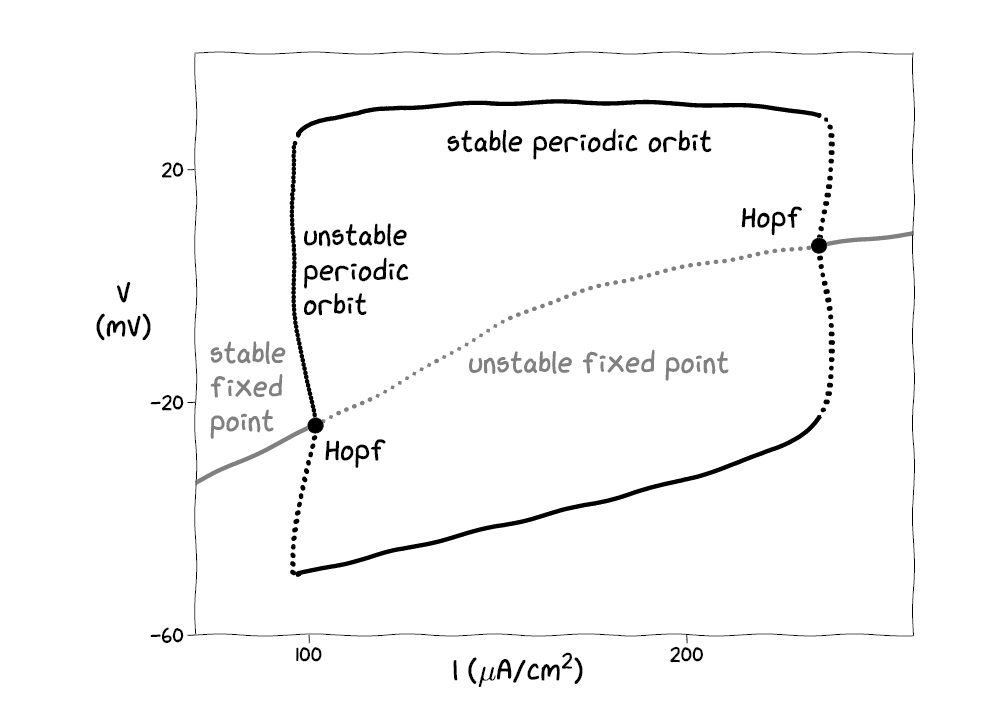
\includegraphics[width=8cm]{MLbifdiag.png}
\end{figure}

Just as equilibrium points can be unstable, so can periodic solutions.
The periodic solutions emerging from the Hopf bifurcations in this case
are unstable and therefore not observable in numerical simulations.
However, they gain stability at turning points. The stable periodic
solutions (limit cycles) are repetative firing. Oscillations emerging
from Hopf bifurcations have small amplitude and a non-zero emergent
frequency proportional to \(\mbox{Im}(\lambda(I_c))\), so there is a
jump from zero to a finite firing frequency typically referred to as
\href{https://neuronaldynamics.epfl.ch/online/Ch4.S4.html}{Type II
firing}. A Hopf bifurcation is also the mechanism giving rise to
oscillations in the Hodgkin-Huxley model we studied above.

    \hypertarget{bistability}{%
\paragraph{Bistability}\label{bistability}}

The bifurcation diagram above also shows a (small) range of \(I\) values
for which both the equilibrium point and the periodic orbit are stable
and an unstable periodic orbit also exists. In this case for different
initial conditions we see different behaviour. For these values of \(I\)
a brief impulse could switch the system out of the oscillatory response
and back to rest.

    \textbf{Exercise 11:} Use the code below to investigate numerically the
behaviour for different values of \(I\). It should agree with the
bifurcation diagram: For \(I=60\) you should observe only the stable
equilibrium point, for \(I=160\) the stable solution is the periodic
orbit, for \(I=260\), the stable solution is again just the steady
state. For \(I=90\) there is bistability between the equilibrium point
and the periodic solution.

    \begin{tcolorbox}[breakable, size=fbox, boxrule=1pt, pad at break*=1mm,colback=cellbackground, colframe=cellborder]
\prompt{In}{incolor}{ }{\boxspacing}
\begin{Verbatim}[commandchars=\\\{\}]
\PY{n}{I}\PY{o}{=}\PY{l+m+mi}{60}

\PY{c+c1}{\PYZsh{} Simulate model for different initial conditions}
\PY{n}{ML\PYZus{}sol1} \PY{o}{=} \PY{n}{solve\PYZus{}ivp}\PY{p}{(}\PY{n}{ML}\PY{p}{,} \PY{p}{[}\PY{l+m+mi}{0}\PY{p}{,}\PY{l+m+mi}{500}\PY{p}{]}\PY{p}{,} \PY{p}{[}\PY{o}{\PYZhy{}}\PY{l+m+mi}{40}\PY{p}{,}\PY{l+m+mf}{0.0}\PY{p}{]}\PY{p}{,} \PY{n}{dense\PYZus{}output} \PY{o}{=} \PY{k+kc}{True}\PY{p}{,} \PY{n}{args} \PY{o}{=} \PY{p}{(}\PY{n}{I}\PY{p}{,}\PY{p}{)}\PY{p}{)}
\PY{n}{ML\PYZus{}sol2} \PY{o}{=} \PY{n}{solve\PYZus{}ivp}\PY{p}{(}\PY{n}{ML}\PY{p}{,} \PY{p}{[}\PY{l+m+mi}{0}\PY{p}{,}\PY{l+m+mi}{500}\PY{p}{]}\PY{p}{,} \PY{p}{[}\PY{o}{\PYZhy{}}\PY{l+m+mi}{20}\PY{p}{,}\PY{l+m+mf}{0.2}\PY{p}{]}\PY{p}{,} \PY{n}{dense\PYZus{}output} \PY{o}{=} \PY{k+kc}{True}\PY{p}{,} \PY{n}{args} \PY{o}{=} \PY{p}{(}\PY{n}{I}\PY{p}{,}\PY{p}{)}\PY{p}{)}
\PY{n}{ML\PYZus{}sol3} \PY{o}{=} \PY{n}{solve\PYZus{}ivp}\PY{p}{(}\PY{n}{ML}\PY{p}{,} \PY{p}{[}\PY{l+m+mi}{0}\PY{p}{,}\PY{l+m+mi}{500}\PY{p}{]}\PY{p}{,} \PY{p}{[}\PY{o}{\PYZhy{}}\PY{l+m+mi}{15}\PY{p}{,}\PY{l+m+mf}{0.0}\PY{p}{]}\PY{p}{,} \PY{n}{dense\PYZus{}output} \PY{o}{=} \PY{k+kc}{True}\PY{p}{,} \PY{n}{args} \PY{o}{=} \PY{p}{(}\PY{n}{I}\PY{p}{,}\PY{p}{)}\PY{p}{)}
\PY{n}{ML\PYZus{}sol4} \PY{o}{=} \PY{n}{solve\PYZus{}ivp}\PY{p}{(}\PY{n}{ML}\PY{p}{,} \PY{p}{[}\PY{l+m+mi}{0}\PY{p}{,}\PY{l+m+mi}{500}\PY{p}{]}\PY{p}{,} \PY{p}{[}\PY{l+m+mi}{20}\PY{p}{,}\PY{l+m+mf}{0.0}\PY{p}{]}\PY{p}{,} \PY{n}{dense\PYZus{}output} \PY{o}{=} \PY{k+kc}{True}\PY{p}{,} \PY{n}{args} \PY{o}{=} \PY{p}{(}\PY{n}{I}\PY{p}{,}\PY{p}{)}\PY{p}{)}
\PY{n}{t\PYZus{}ML} \PY{o}{=} \PY{n}{np}\PY{o}{.}\PY{n}{linspace}\PY{p}{(}\PY{l+m+mi}{0}\PY{p}{,} \PY{l+m+mi}{500}\PY{p}{,} \PY{l+m+mi}{10000}\PY{p}{)}
\PY{n}{x\PYZus{}ML1} \PY{o}{=} \PY{n}{ML\PYZus{}sol1}\PY{o}{.}\PY{n}{sol}\PY{p}{(}\PY{n}{t\PYZus{}ML}\PY{p}{)}
\PY{n}{x\PYZus{}ML2} \PY{o}{=} \PY{n}{ML\PYZus{}sol2}\PY{o}{.}\PY{n}{sol}\PY{p}{(}\PY{n}{t\PYZus{}ML}\PY{p}{)}
\PY{n}{x\PYZus{}ML3} \PY{o}{=} \PY{n}{ML\PYZus{}sol3}\PY{o}{.}\PY{n}{sol}\PY{p}{(}\PY{n}{t\PYZus{}ML}\PY{p}{)}
\PY{n}{x\PYZus{}ML4} \PY{o}{=} \PY{n}{ML\PYZus{}sol4}\PY{o}{.}\PY{n}{sol}\PY{p}{(}\PY{n}{t\PYZus{}ML}\PY{p}{)}



\PY{c+c1}{\PYZsh{} plot trajectories in (V, w) plane}

\PY{n}{plt}\PY{o}{.}\PY{n}{figure}\PY{p}{(}\PY{n}{figsize}\PY{o}{=}\PY{p}{(}\PY{l+m+mi}{12}\PY{p}{,}\PY{l+m+mi}{8}\PY{p}{)}\PY{p}{)}
\PY{n}{plt}\PY{o}{.}\PY{n}{plot}\PY{p}{(} \PY{n}{x\PYZus{}ML1}\PY{p}{[}\PY{l+m+mi}{0}\PY{p}{]}\PY{p}{,} \PY{n}{x\PYZus{}ML1}\PY{p}{[}\PY{l+m+mi}{1}\PY{p}{]}\PY{p}{,}\PY{n}{linewidth}\PY{o}{=}\PY{l+m+mi}{2}\PY{p}{)}
\PY{n}{plt}\PY{o}{.}\PY{n}{plot}\PY{p}{(} \PY{n}{x\PYZus{}ML2}\PY{p}{[}\PY{l+m+mi}{0}\PY{p}{]}\PY{p}{,} \PY{n}{x\PYZus{}ML2}\PY{p}{[}\PY{l+m+mi}{1}\PY{p}{]}\PY{p}{,}\PY{n}{linewidth}\PY{o}{=}\PY{l+m+mi}{2}\PY{p}{)}
\PY{n}{plt}\PY{o}{.}\PY{n}{plot}\PY{p}{(} \PY{n}{x\PYZus{}ML3}\PY{p}{[}\PY{l+m+mi}{0}\PY{p}{]}\PY{p}{,} \PY{n}{x\PYZus{}ML3}\PY{p}{[}\PY{l+m+mi}{1}\PY{p}{]}\PY{p}{,}\PY{n}{linewidth}\PY{o}{=}\PY{l+m+mi}{2}\PY{p}{)}
\PY{n}{plt}\PY{o}{.}\PY{n}{plot}\PY{p}{(} \PY{n}{x\PYZus{}ML4}\PY{p}{[}\PY{l+m+mi}{0}\PY{p}{]}\PY{p}{,} \PY{n}{x\PYZus{}ML4}\PY{p}{[}\PY{l+m+mi}{1}\PY{p}{]}\PY{p}{,}\PY{n}{linewidth}\PY{o}{=}\PY{l+m+mi}{2}\PY{p}{)}

\PY{n}{delta} \PY{o}{=} \PY{l+m+mf}{0.025}

\PY{n}{xrange} \PY{o}{=} \PY{n}{np}\PY{o}{.}\PY{n}{arange}\PY{p}{(}\PY{o}{\PYZhy{}}\PY{l+m+mi}{80}\PY{p}{,} \PY{l+m+mi}{60}\PY{p}{,} \PY{n}{delta}\PY{p}{)}
\PY{n}{yrange} \PY{o}{=} \PY{n}{np}\PY{o}{.}\PY{n}{arange}\PY{p}{(}\PY{o}{\PYZhy{}}\PY{l+m+mf}{0.1}\PY{p}{,} \PY{l+m+mf}{0.8}\PY{p}{,} \PY{n}{delta}\PY{p}{)}
\PY{n}{Vn}\PY{p}{,} \PY{n}{wn} \PY{o}{=} \PY{n}{np}\PY{o}{.}\PY{n}{meshgrid}\PY{p}{(}\PY{n}{xrange}\PY{p}{,}\PY{n}{yrange}\PY{p}{)}

\PY{n}{F} \PY{o}{=} \PY{p}{(}\PY{l+m+mi}{1}\PY{o}{/}\PY{n}{C}\PY{p}{)}\PY{o}{*}\PY{p}{(}\PY{n}{I} \PY{o}{\PYZhy{}} \PY{n}{gCa}\PY{o}{*}\PY{l+m+mf}{0.5}\PY{o}{*}\PY{p}{(}\PY{l+m+mi}{1}\PY{o}{+}\PY{n}{np}\PY{o}{.}\PY{n}{tanh}\PY{p}{(}\PY{p}{(}\PY{n}{Vn}\PY{o}{\PYZhy{}}\PY{n}{V1}\PY{p}{)}\PY{o}{/}\PY{n}{V2}\PY{p}{)}\PY{p}{)}\PY{o}{*}\PY{p}{(}\PY{n}{Vn}\PY{o}{\PYZhy{}}\PY{n}{VCa}\PY{p}{)} \PY{o}{\PYZhy{}} \PY{n}{gK}\PY{o}{*}\PY{n}{wn}\PY{o}{*}\PY{p}{(}\PY{n}{Vn}\PY{o}{\PYZhy{}}\PY{n}{VK}\PY{p}{)} \PY{o}{\PYZhy{}} \PY{n}{gL}\PY{o}{*}\PY{p}{(}\PY{n}{Vn}\PY{o}{\PYZhy{}}\PY{n}{VL}\PY{p}{)}\PY{p}{)}\PY{p}{;}
\PY{n}{G} \PY{o}{=}  \PY{n}{phi}\PY{o}{*}\PY{p}{(}\PY{l+m+mf}{0.5}\PY{o}{*}\PY{p}{(}\PY{l+m+mi}{1}\PY{o}{+}\PY{n}{np}\PY{o}{.}\PY{n}{tanh}\PY{p}{(}\PY{p}{(}\PY{n}{Vn}\PY{o}{\PYZhy{}}\PY{n}{V3}\PY{p}{)}\PY{o}{/}\PY{n}{V4}\PY{p}{)}\PY{p}{)}\PY{o}{\PYZhy{}}\PY{n}{wn}\PY{p}{)}\PY{o}{/}\PY{p}{(}\PY{l+m+mi}{1}\PY{o}{/}\PY{p}{(}\PY{n}{np}\PY{o}{.}\PY{n}{cosh}\PY{p}{(}\PY{p}{(}\PY{n}{Vn}\PY{o}{\PYZhy{}}\PY{n}{V3}\PY{p}{)}\PY{o}{/}\PY{p}{(}\PY{l+m+mi}{2}\PY{o}{*}\PY{n}{V4}\PY{p}{)}\PY{p}{)}\PY{p}{)}\PY{p}{)}\PY{p}{;}

\PY{c+c1}{\PYZsh{}plot nullclines}
\PY{n}{plt}\PY{o}{.}\PY{n}{contour}\PY{p}{(}\PY{n}{Vn}\PY{p}{,} \PY{n}{wn}\PY{p}{,} \PY{n}{F}\PY{p}{,} \PY{p}{[}\PY{l+m+mi}{0}\PY{p}{]}\PY{p}{)}
\PY{n}{plt}\PY{o}{.}\PY{n}{contour}\PY{p}{(}\PY{n}{Vn}\PY{p}{,} \PY{n}{wn}\PY{p}{,} \PY{n}{G}\PY{p}{,} \PY{p}{[}\PY{l+m+mi}{0}\PY{p}{]}\PY{p}{)}

\PY{n}{plt}\PY{o}{.}\PY{n}{ylabel}\PY{p}{(}\PY{l+s+s2}{\PYZdq{}}\PY{l+s+s2}{Potassium gating variable (w)}\PY{l+s+s2}{\PYZdq{}}\PY{p}{)}
\PY{n}{plt}\PY{o}{.}\PY{n}{xlabel}\PY{p}{(}\PY{l+s+s2}{\PYZdq{}}\PY{l+s+s2}{membrane voltage V (mV)}\PY{l+s+s2}{\PYZdq{}}\PY{p}{)}
\PY{n}{plt}\PY{o}{.}\PY{n}{show}\PY{p}{(}\PY{p}{)}
\end{Verbatim}
\end{tcolorbox}

    You can use the code below to plot a particular solution against time.

    \begin{tcolorbox}[breakable, size=fbox, boxrule=1pt, pad at break*=1mm,colback=cellbackground, colframe=cellborder]
\prompt{In}{incolor}{ }{\boxspacing}
\begin{Verbatim}[commandchars=\\\{\}]
\PY{c+c1}{\PYZsh{} plot variables against time}
\PY{n}{fig}\PY{p}{,} \PY{n}{ax1} \PY{o}{=} \PY{n}{plt}\PY{o}{.}\PY{n}{subplots}\PY{p}{(}\PY{p}{)}

\PY{n}{color} \PY{o}{=} \PY{l+s+s1}{\PYZsq{}}\PY{l+s+s1}{tab:blue}\PY{l+s+s1}{\PYZsq{}}
\PY{n}{ax1}\PY{o}{.}\PY{n}{set\PYZus{}xlabel}\PY{p}{(}\PY{l+s+s1}{\PYZsq{}}\PY{l+s+s1}{time (ms)}\PY{l+s+s1}{\PYZsq{}}\PY{p}{)}
\PY{n}{ax1}\PY{o}{.}\PY{n}{set\PYZus{}ylabel}\PY{p}{(}\PY{l+s+s1}{\PYZsq{}}\PY{l+s+s1}{Voltage (mV)}\PY{l+s+s1}{\PYZsq{}}\PY{p}{,} \PY{n}{color}\PY{o}{=}\PY{n}{color}\PY{p}{)}
\PY{n}{ax1}\PY{o}{.}\PY{n}{plot}\PY{p}{(}\PY{n}{t\PYZus{}ML}\PY{p}{,} \PY{n}{x\PYZus{}ML2}\PY{p}{[}\PY{l+m+mi}{0}\PY{p}{]}\PY{p}{,} \PY{n}{color}\PY{o}{=}\PY{n}{color}\PY{p}{)}
\PY{n}{ax1}\PY{o}{.}\PY{n}{tick\PYZus{}params}\PY{p}{(}\PY{n}{axis}\PY{o}{=}\PY{l+s+s1}{\PYZsq{}}\PY{l+s+s1}{y}\PY{l+s+s1}{\PYZsq{}}\PY{p}{,} \PY{n}{labelcolor}\PY{o}{=}\PY{n}{color}\PY{p}{)}

\PY{n}{ax2} \PY{o}{=} \PY{n}{ax1}\PY{o}{.}\PY{n}{twinx}\PY{p}{(}\PY{p}{)}

\PY{n}{color} \PY{o}{=} \PY{l+s+s1}{\PYZsq{}}\PY{l+s+s1}{tab:gray}\PY{l+s+s1}{\PYZsq{}}
\PY{n}{ax2}\PY{o}{.}\PY{n}{plot}\PY{p}{(}\PY{n}{t\PYZus{}ML}\PY{p}{,} \PY{n}{x\PYZus{}ML2}\PY{p}{[}\PY{l+m+mi}{1}\PY{p}{]}\PY{p}{,} \PY{n}{color}\PY{o}{=}\PY{n}{color}\PY{p}{,} \PY{n}{linestyle}\PY{o}{=}\PY{l+s+s1}{\PYZsq{}}\PY{l+s+s1}{solid}\PY{l+s+s1}{\PYZsq{}}\PY{p}{)}
\PY{n}{ax2}\PY{o}{.}\PY{n}{set\PYZus{}ylabel}\PY{p}{(}\PY{l+s+s1}{\PYZsq{}}\PY{l+s+s1}{w}\PY{l+s+s1}{\PYZsq{}}\PY{p}{,} \PY{n}{color}\PY{o}{=}\PY{n}{color}\PY{p}{)}
\PY{n}{ax2}\PY{o}{.}\PY{n}{tick\PYZus{}params}\PY{p}{(}\PY{n}{axis}\PY{o}{=}\PY{l+s+s1}{\PYZsq{}}\PY{l+s+s1}{y}\PY{l+s+s1}{\PYZsq{}}\PY{p}{,} \PY{n}{labelcolor}\PY{o}{=}\PY{n}{color}\PY{p}{)}

\PY{n}{plt}\PY{o}{.}\PY{n}{show}\PY{p}{(}\PY{p}{)}
\end{Verbatim}
\end{tcolorbox}

    \hypertarget{oscillations-emerging-with-zero-frequency-global-bifurcations}{%
\subsubsection{Oscillations emerging with zero frequency (global
bifurcations)}\label{oscillations-emerging-with-zero-frequency-global-bifurcations}}

More usual than type II firing is the observation of periodic firing
with low frequencies at onset (type I). We now briefly outline two
mechanisms for generating such periodic behaviour.

\hypertarget{snic-bifurcation}{%
\paragraph{SNIC bifurcation}\label{snic-bifurcation}}

If \(F(V, w_\infty(V))\) is non-monotonic (has turning points) then the
system can simultaneously have more than one equilibrium point. For
example if we change some of the parameters we can get the phase
portrait below with three equilibrium points, one stable, one unstable
and one \href{https://en.wikipedia.org/wiki/Equilibrium_point}{saddle}.
(A saddle point has one positive real eigenvalue and one negative real
eigenvalue so trajectories appproach in one direction and move away in
the other). There are two trajectories that leave the saddle and both
connect to the stable equilibrium point, one goes directly there and one
goes around the unstable equilibrium.

\begin{figure}
  \centering
  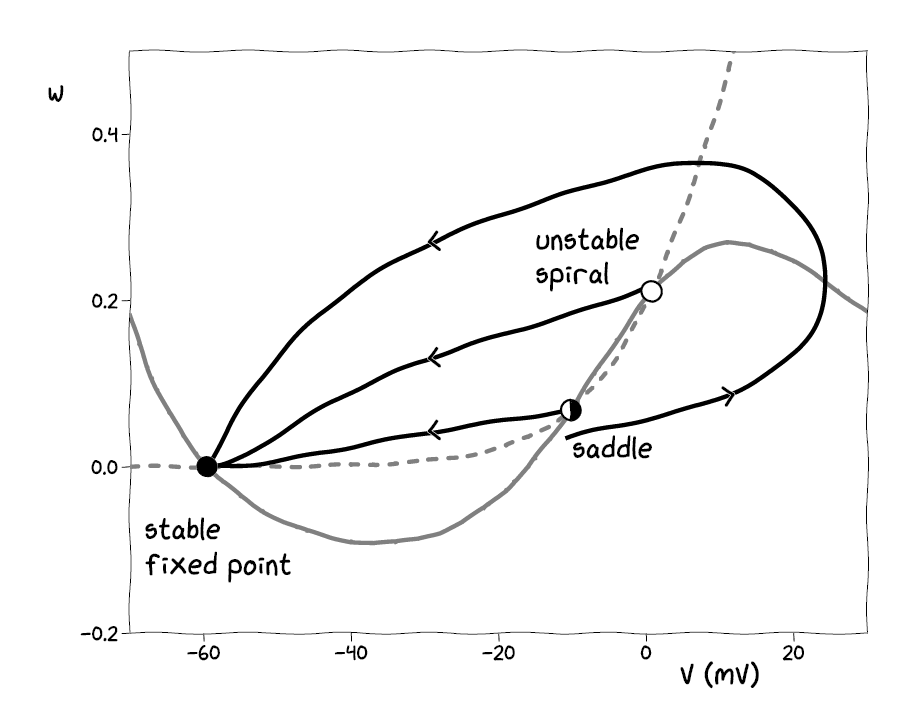
\includegraphics[width=8cm]{SNIC.png}
\end{figure}

Increasing \(I\) moves the \(V\)-nullcline upwards, making the stable
equilibrium and the saddle closer together until they annihilate each
other when \(I=I_c\) and then disappear leaving a limit cycle for
\(I>I_c\). This situation is called a \textbf{saddle node on an
invariant circle (SNIC) bifurcation}. At \(I=I_c\) the limit cycle has
infinite period (it is a
\href{https://en.wikipedia.org/wiki/Homoclinic_orbit}{homoclinic orbit})
so the frequency is zero. For \(I\) just above \(I_c\) the frequency of
the periodic orbit scales as \(\sqrt{I-I_c}\)

\textbf{Exercise 12:} Use the code below to see how the limit cycle
comes into existence when the equilibrium points annihilate.

    \begin{tcolorbox}[breakable, size=fbox, boxrule=1pt, pad at break*=1mm,colback=cellbackground, colframe=cellborder]
\prompt{In}{incolor}{ }{\boxspacing}
\begin{Verbatim}[commandchars=\\\{\}]
\PY{c+c1}{\PYZsh{} Define new parameter values }
\PY{n}{V3}\PY{o}{=}\PY{l+m+mi}{12}
\PY{n}{V4}\PY{o}{=}\PY{l+m+mi}{17}
\PY{n}{phi} \PY{o}{=} \PY{l+m+mi}{2}\PY{o}{/}\PY{l+m+mi}{30}

\PY{c+c1}{\PYZsh{} F(V, w\PYZus{}inf(V)) is non\PYZhy{}monotonic}

\PY{n}{Vss} \PY{o}{=} \PY{n}{np}\PY{o}{.}\PY{n}{linspace}\PY{p}{(}\PY{o}{\PYZhy{}}\PY{l+m+mi}{60}\PY{p}{,}\PY{l+m+mi}{10}\PY{p}{,}\PY{l+m+mi}{1000}\PY{p}{)}
\PY{n}{F} \PY{o}{=}  \PY{n}{gCa}\PY{o}{*}\PY{l+m+mf}{0.5}\PY{o}{*}\PY{p}{(}\PY{l+m+mi}{1}\PY{o}{+}\PY{n}{np}\PY{o}{.}\PY{n}{tanh}\PY{p}{(}\PY{p}{(}\PY{n}{Vss}\PY{o}{\PYZhy{}}\PY{n}{V1}\PY{p}{)}\PY{o}{/}\PY{n}{V2}\PY{p}{)}\PY{p}{)}\PY{o}{*}\PY{p}{(}\PY{n}{Vss}\PY{o}{\PYZhy{}}\PY{n}{VCa}\PY{p}{)} \PY{o}{+} \PY{n}{gK}\PY{o}{*}\PY{l+m+mf}{0.5}\PY{o}{*}\PY{p}{(}\PY{l+m+mi}{1}\PY{o}{+}\PY{n}{np}\PY{o}{.}\PY{n}{tanh}\PY{p}{(}\PY{p}{(}\PY{n}{Vss}\PY{o}{\PYZhy{}}\PY{n}{V3}\PY{p}{)}\PY{o}{/}\PY{n}{V4}\PY{p}{)}\PY{p}{)}\PY{o}{*}\PY{p}{(}\PY{n}{Vss}\PY{o}{\PYZhy{}}\PY{n}{VK}\PY{p}{)} \PY{o}{+} \PY{n}{gL}\PY{o}{*}\PY{p}{(}\PY{n}{Vss}\PY{o}{\PYZhy{}}\PY{n}{VL}\PY{p}{)}
\PY{n}{plt}\PY{o}{.}\PY{n}{figure}\PY{p}{(}\PY{p}{)}
\PY{n}{plt}\PY{o}{.}\PY{n}{plot}\PY{p}{(}\PY{n}{Vss}\PY{p}{,}\PY{n}{F}\PY{p}{)}
\PY{n}{plt}\PY{o}{.}\PY{n}{xlabel}\PY{p}{(}\PY{l+s+s1}{\PYZsq{}}\PY{l+s+s1}{V}\PY{l+s+s1}{\PYZsq{}}\PY{p}{)}
\PY{n}{plt}\PY{o}{.}\PY{n}{ylabel}\PY{p}{(}\PY{l+s+s1}{\PYZsq{}}\PY{l+s+s1}{\PYZdl{}I\PYZus{}}\PY{l+s+si}{\PYZob{}ss\PYZcb{}}\PY{l+s+s1}{ = \PYZhy{}F(V, w\PYZus{}}\PY{l+s+s1}{\PYZbs{}}\PY{l+s+s1}{infty(V))\PYZdl{}}\PY{l+s+s1}{\PYZsq{}}\PY{p}{)}
\PY{n}{plt}\PY{o}{.}\PY{n}{show}\PY{p}{(}\PY{p}{)}

\PY{c+c1}{\PYZsh{} try I=0, I=39 (just after SNIC), I=90 (bistability), I=120, stable equilibrium }
\PY{n}{I}\PY{o}{=}\PY{l+m+mi}{39}

\PY{c+c1}{\PYZsh{} Simulate model for different initial conditions}
\PY{n}{ML\PYZus{}sol1} \PY{o}{=} \PY{n}{solve\PYZus{}ivp}\PY{p}{(}\PY{n}{ML}\PY{p}{,} \PY{p}{[}\PY{l+m+mi}{0}\PY{p}{,}\PY{l+m+mi}{500}\PY{p}{]}\PY{p}{,} \PY{p}{[}\PY{l+m+mi}{0}\PY{p}{,}\PY{l+m+mf}{0.3}\PY{p}{]}\PY{p}{,} \PY{n}{dense\PYZus{}output} \PY{o}{=} \PY{k+kc}{True}\PY{p}{,} \PY{n}{args} \PY{o}{=} \PY{p}{(}\PY{n}{I}\PY{p}{,}\PY{p}{)}\PY{p}{)}
\PY{n}{ML\PYZus{}sol2} \PY{o}{=} \PY{n}{solve\PYZus{}ivp}\PY{p}{(}\PY{n}{ML}\PY{p}{,} \PY{p}{[}\PY{l+m+mi}{0}\PY{p}{,}\PY{l+m+mi}{500}\PY{p}{]}\PY{p}{,} \PY{p}{[}\PY{o}{\PYZhy{}}\PY{l+m+mi}{15}\PY{p}{,}\PY{l+m+mf}{0.03}\PY{p}{]}\PY{p}{,} \PY{n}{dense\PYZus{}output} \PY{o}{=} \PY{k+kc}{True}\PY{p}{,} \PY{n}{args} \PY{o}{=} \PY{p}{(}\PY{n}{I}\PY{p}{,}\PY{p}{)}\PY{p}{)}
\PY{n}{ML\PYZus{}sol3} \PY{o}{=} \PY{n}{solve\PYZus{}ivp}\PY{p}{(}\PY{n}{ML}\PY{p}{,} \PY{p}{[}\PY{l+m+mi}{0}\PY{p}{,}\PY{l+m+mi}{500}\PY{p}{]}\PY{p}{,} \PY{p}{[}\PY{o}{\PYZhy{}}\PY{l+m+mi}{14}\PY{p}{,}\PY{l+m+mf}{0.03}\PY{p}{]}\PY{p}{,} \PY{n}{dense\PYZus{}output} \PY{o}{=} \PY{k+kc}{True}\PY{p}{,} \PY{n}{args} \PY{o}{=} \PY{p}{(}\PY{n}{I}\PY{p}{,}\PY{p}{)}\PY{p}{)}
\PY{n}{ML\PYZus{}sol4} \PY{o}{=} \PY{n}{solve\PYZus{}ivp}\PY{p}{(}\PY{n}{ML}\PY{p}{,} \PY{p}{[}\PY{l+m+mi}{0}\PY{p}{,}\PY{l+m+mi}{500}\PY{p}{]}\PY{p}{,} \PY{p}{[}\PY{l+m+mi}{20}\PY{p}{,}\PY{l+m+mf}{0.0}\PY{p}{]}\PY{p}{,} \PY{n}{dense\PYZus{}output} \PY{o}{=} \PY{k+kc}{True}\PY{p}{,} \PY{n}{args} \PY{o}{=} \PY{p}{(}\PY{n}{I}\PY{p}{,}\PY{p}{)}\PY{p}{)}
\PY{n}{t\PYZus{}ML} \PY{o}{=} \PY{n}{np}\PY{o}{.}\PY{n}{linspace}\PY{p}{(}\PY{l+m+mi}{0}\PY{p}{,} \PY{l+m+mi}{500}\PY{p}{,} \PY{l+m+mi}{10000}\PY{p}{)}
\PY{n}{x\PYZus{}ML1} \PY{o}{=} \PY{n}{ML\PYZus{}sol1}\PY{o}{.}\PY{n}{sol}\PY{p}{(}\PY{n}{t\PYZus{}ML}\PY{p}{)}
\PY{n}{x\PYZus{}ML2} \PY{o}{=} \PY{n}{ML\PYZus{}sol2}\PY{o}{.}\PY{n}{sol}\PY{p}{(}\PY{n}{t\PYZus{}ML}\PY{p}{)}
\PY{n}{x\PYZus{}ML3} \PY{o}{=} \PY{n}{ML\PYZus{}sol3}\PY{o}{.}\PY{n}{sol}\PY{p}{(}\PY{n}{t\PYZus{}ML}\PY{p}{)}
\PY{n}{x\PYZus{}ML4} \PY{o}{=} \PY{n}{ML\PYZus{}sol4}\PY{o}{.}\PY{n}{sol}\PY{p}{(}\PY{n}{t\PYZus{}ML}\PY{p}{)}


\PY{c+c1}{\PYZsh{} plot trajectories in (V, w) plane}

\PY{n}{plt}\PY{o}{.}\PY{n}{figure}\PY{p}{(}\PY{p}{)}
\PY{n}{plt}\PY{o}{.}\PY{n}{plot}\PY{p}{(} \PY{n}{x\PYZus{}ML1}\PY{p}{[}\PY{l+m+mi}{0}\PY{p}{]}\PY{p}{,} \PY{n}{x\PYZus{}ML1}\PY{p}{[}\PY{l+m+mi}{1}\PY{p}{]}\PY{p}{,}\PY{n}{linewidth}\PY{o}{=}\PY{l+m+mi}{2}\PY{p}{)}
\PY{n}{plt}\PY{o}{.}\PY{n}{plot}\PY{p}{(} \PY{n}{x\PYZus{}ML2}\PY{p}{[}\PY{l+m+mi}{0}\PY{p}{]}\PY{p}{,} \PY{n}{x\PYZus{}ML2}\PY{p}{[}\PY{l+m+mi}{1}\PY{p}{]}\PY{p}{,}\PY{n}{linewidth}\PY{o}{=}\PY{l+m+mi}{2}\PY{p}{)}
\PY{n}{plt}\PY{o}{.}\PY{n}{plot}\PY{p}{(} \PY{n}{x\PYZus{}ML3}\PY{p}{[}\PY{l+m+mi}{0}\PY{p}{]}\PY{p}{,} \PY{n}{x\PYZus{}ML3}\PY{p}{[}\PY{l+m+mi}{1}\PY{p}{]}\PY{p}{,}\PY{n}{linewidth}\PY{o}{=}\PY{l+m+mi}{2}\PY{p}{)}
\PY{n}{plt}\PY{o}{.}\PY{n}{plot}\PY{p}{(} \PY{n}{x\PYZus{}ML4}\PY{p}{[}\PY{l+m+mi}{0}\PY{p}{]}\PY{p}{,} \PY{n}{x\PYZus{}ML4}\PY{p}{[}\PY{l+m+mi}{1}\PY{p}{]}\PY{p}{,}\PY{n}{linewidth}\PY{o}{=}\PY{l+m+mi}{2}\PY{p}{)}

\PY{n}{delta} \PY{o}{=} \PY{l+m+mf}{0.025}

\PY{n}{xrange} \PY{o}{=} \PY{n}{np}\PY{o}{.}\PY{n}{arange}\PY{p}{(}\PY{o}{\PYZhy{}}\PY{l+m+mi}{80}\PY{p}{,} \PY{l+m+mi}{60}\PY{p}{,} \PY{n}{delta}\PY{p}{)}
\PY{n}{yrange} \PY{o}{=} \PY{n}{np}\PY{o}{.}\PY{n}{arange}\PY{p}{(}\PY{o}{\PYZhy{}}\PY{l+m+mf}{0.1}\PY{p}{,} \PY{l+m+mf}{0.8}\PY{p}{,} \PY{n}{delta}\PY{p}{)}
\PY{n}{Vn}\PY{p}{,} \PY{n}{wn} \PY{o}{=} \PY{n}{np}\PY{o}{.}\PY{n}{meshgrid}\PY{p}{(}\PY{n}{xrange}\PY{p}{,}\PY{n}{yrange}\PY{p}{)}

\PY{n}{F} \PY{o}{=} \PY{p}{(}\PY{l+m+mi}{1}\PY{o}{/}\PY{n}{C}\PY{p}{)}\PY{o}{*}\PY{p}{(}\PY{n}{I} \PY{o}{\PYZhy{}} \PY{n}{gCa}\PY{o}{*}\PY{l+m+mf}{0.5}\PY{o}{*}\PY{p}{(}\PY{l+m+mi}{1}\PY{o}{+}\PY{n}{np}\PY{o}{.}\PY{n}{tanh}\PY{p}{(}\PY{p}{(}\PY{n}{Vn}\PY{o}{\PYZhy{}}\PY{n}{V1}\PY{p}{)}\PY{o}{/}\PY{n}{V2}\PY{p}{)}\PY{p}{)}\PY{o}{*}\PY{p}{(}\PY{n}{Vn}\PY{o}{\PYZhy{}}\PY{n}{VCa}\PY{p}{)} \PY{o}{\PYZhy{}} \PY{n}{gK}\PY{o}{*}\PY{n}{wn}\PY{o}{*}\PY{p}{(}\PY{n}{Vn}\PY{o}{\PYZhy{}}\PY{n}{VK}\PY{p}{)} \PY{o}{\PYZhy{}} \PY{n}{gL}\PY{o}{*}\PY{p}{(}\PY{n}{Vn}\PY{o}{\PYZhy{}}\PY{n}{VL}\PY{p}{)}\PY{p}{)}\PY{p}{;}
\PY{n}{G} \PY{o}{=}  \PY{n}{phi}\PY{o}{*}\PY{p}{(}\PY{l+m+mf}{0.5}\PY{o}{*}\PY{p}{(}\PY{l+m+mi}{1}\PY{o}{+}\PY{n}{np}\PY{o}{.}\PY{n}{tanh}\PY{p}{(}\PY{p}{(}\PY{n}{Vn}\PY{o}{\PYZhy{}}\PY{n}{V3}\PY{p}{)}\PY{o}{/}\PY{n}{V4}\PY{p}{)}\PY{p}{)}\PY{o}{\PYZhy{}}\PY{n}{wn}\PY{p}{)}\PY{o}{/}\PY{p}{(}\PY{l+m+mi}{1}\PY{o}{/}\PY{p}{(}\PY{n}{np}\PY{o}{.}\PY{n}{cosh}\PY{p}{(}\PY{p}{(}\PY{n}{Vn}\PY{o}{\PYZhy{}}\PY{n}{V3}\PY{p}{)}\PY{o}{/}\PY{p}{(}\PY{l+m+mi}{2}\PY{o}{*}\PY{n}{V4}\PY{p}{)}\PY{p}{)}\PY{p}{)}\PY{p}{)}\PY{p}{;}

\PY{c+c1}{\PYZsh{}plot nullclines}
\PY{n}{plt}\PY{o}{.}\PY{n}{contour}\PY{p}{(}\PY{n}{Vn}\PY{p}{,} \PY{n}{wn}\PY{p}{,} \PY{n}{F}\PY{p}{,} \PY{p}{[}\PY{l+m+mi}{0}\PY{p}{]}\PY{p}{)}
\PY{n}{plt}\PY{o}{.}\PY{n}{contour}\PY{p}{(}\PY{n}{Vn}\PY{p}{,} \PY{n}{wn}\PY{p}{,} \PY{n}{G}\PY{p}{,} \PY{p}{[}\PY{l+m+mi}{0}\PY{p}{]}\PY{p}{)}

\PY{n}{plt}\PY{o}{.}\PY{n}{ylabel}\PY{p}{(}\PY{l+s+s2}{\PYZdq{}}\PY{l+s+s2}{Potassium gating variable (w)}\PY{l+s+s2}{\PYZdq{}}\PY{p}{)}
\PY{n}{plt}\PY{o}{.}\PY{n}{xlabel}\PY{p}{(}\PY{l+s+s2}{\PYZdq{}}\PY{l+s+s2}{membrane voltage V (mV)}\PY{l+s+s2}{\PYZdq{}}\PY{p}{)}
\PY{n}{plt}\PY{o}{.}\PY{n}{show}\PY{p}{(}\PY{p}{)}
\end{Verbatim}
\end{tcolorbox}

    The corresponding bifurcation diagram is as below.
    
    \begin{figure}[!h]
  \centering
  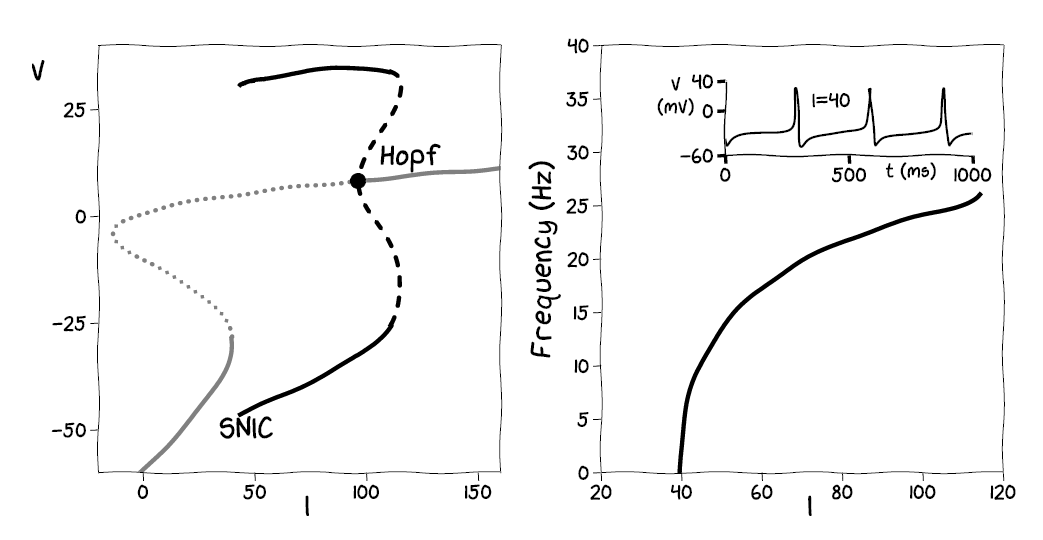
\includegraphics[width=8cm]{SNICbif.png}
\end{figure}

    \textbf{Homoclinic bifurcation} There is another way that oscillations
with low frequency at onset can be created in the Morris-Lecar model.
For intermediate values of \(\phi\), it is possible for both the lower
and upper equilibrium points to be simultaneously stable for some values
of \(I\) with the third a saddle point. The upper branch can lose
stability through a Hopf bifurcation with decreasing \(I\) giving rise
to an unstable periodic solution. This turns and become stable and for
some window of \(I\) there are three steady states (two stable) and two
periodic orbits (one stable). Further decreasing \(I\) the stable
periodic orbit can intercept the saddle, terminating the periodic branch
in a \textbf{homoclinic bifurcation} at \(I=I_c\). At the bifurcation
point a trajectory leaves the saddle in its unstable direction and
returns along its stable direction. The frequency of oscillations scales
as \(1/|\ln(I-I_c)|\). The bifurcation diagram is shown below.

   \begin{figure}[!h]
  \centering
  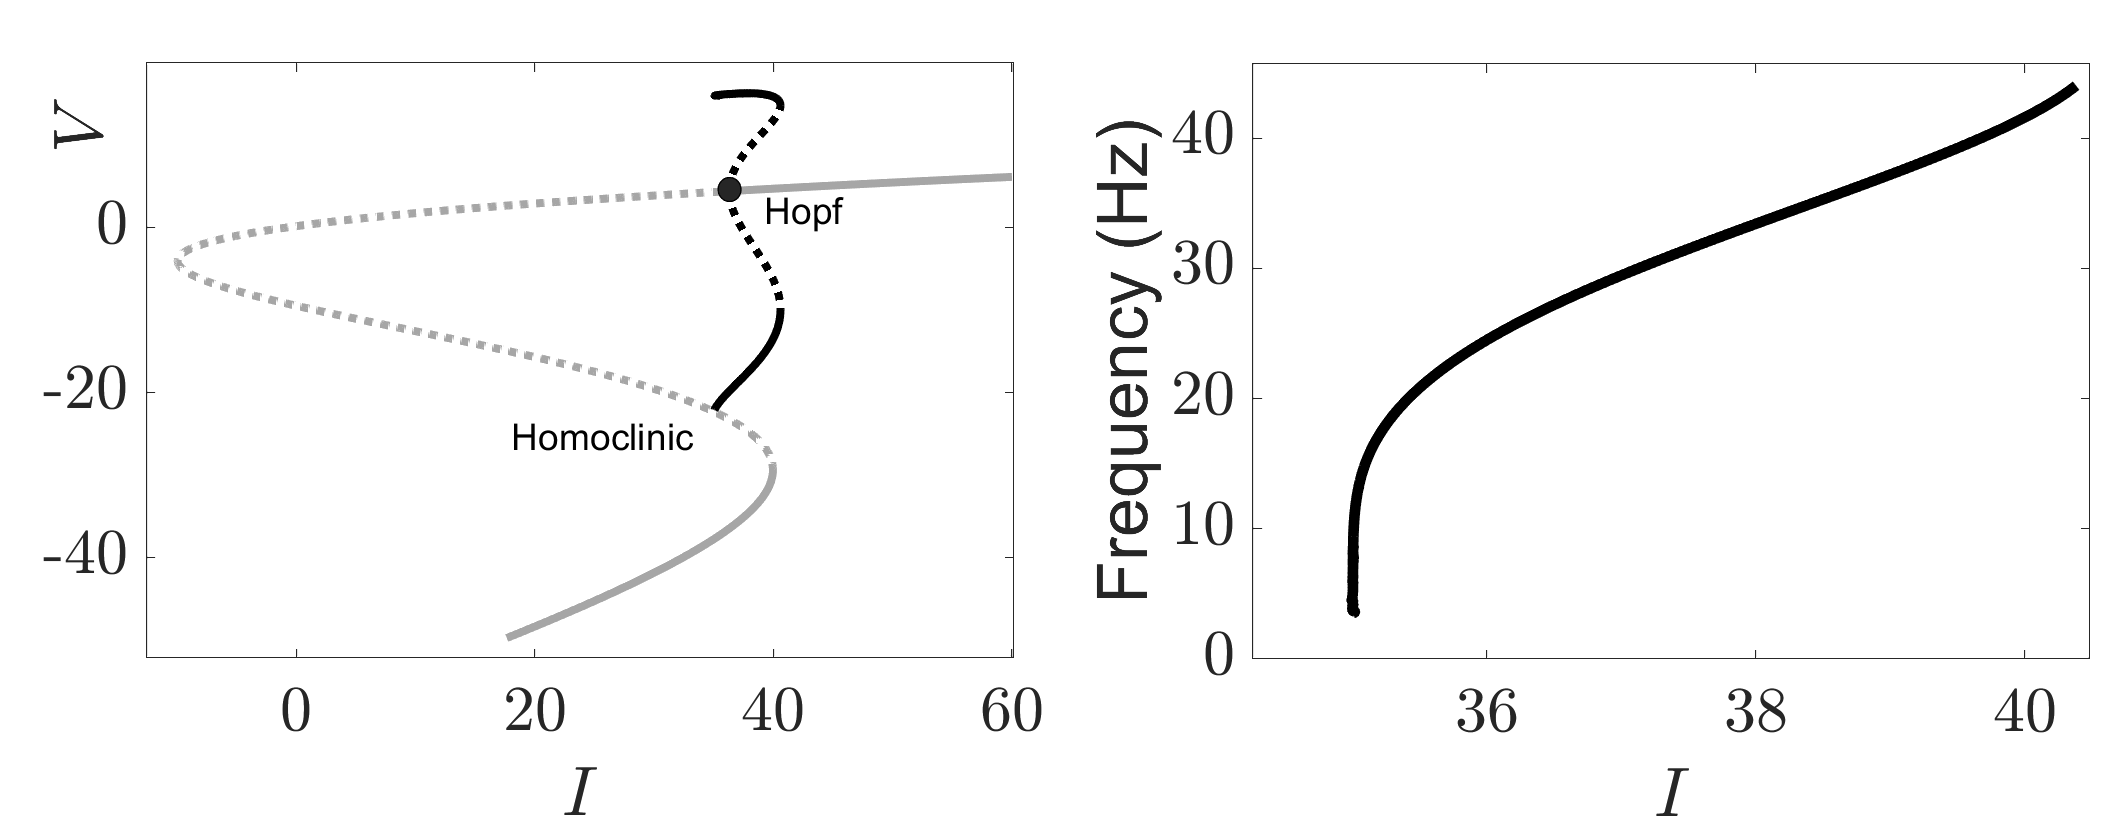
\includegraphics[width=10cm]{MLhomoclinic.png}
\end{figure}

\textbf{Exercise 13:} Use the code below to explore the region of bi/tri
stability between equilibrium points and the periodic solution between
\(I=35\) and \(I=40.6\) for the parameter values given.

    \begin{tcolorbox}[breakable, size=fbox, boxrule=1pt, pad at break*=1mm,colback=cellbackground, colframe=cellborder]
\prompt{In}{incolor}{ }{\boxspacing}
\begin{Verbatim}[commandchars=\\\{\}]
\PY{c+c1}{\PYZsh{} Define new parameter values }
\PY{n}{V3}\PY{o}{=}\PY{l+m+mi}{12}
\PY{n}{V4}\PY{o}{=}\PY{l+m+mf}{17.4}
\PY{n}{phi}\PY{o}{=}\PY{l+m+mf}{0.23}
\PY{n}{gCa}\PY{o}{=}\PY{l+m+mi}{4}

\PY{c+c1}{\PYZsh{}I=34 \PYZsh{} all trajectories go to lower eqm}
\PY{c+c1}{\PYZsh{}I = 35.5 \PYZsh{} bistability between lower eqm and periodic solution}
\PY{c+c1}{\PYZsh{}I=39 \PYZsh{}two eqm and one periodic solution stable}
\PY{n}{I}\PY{o}{=}\PY{l+m+mf}{40.3} \PY{c+c1}{\PYZsh{} bistability between upper eq and periodic solution}
\PY{c+c1}{\PYZsh{}I=50 \PYZsh{} all trajectories go to upper eqm}

\PY{c+c1}{\PYZsh{} Simulate model for different initial conditions}
\PY{n}{ML\PYZus{}sol1} \PY{o}{=} \PY{n}{solve\PYZus{}ivp}\PY{p}{(}\PY{n}{ML}\PY{p}{,} \PY{p}{[}\PY{l+m+mi}{0}\PY{p}{,}\PY{l+m+mi}{1000}\PY{p}{]}\PY{p}{,} \PY{p}{[}\PY{l+m+mi}{3}\PY{p}{,}\PY{l+m+mf}{0.3}\PY{p}{]}\PY{p}{,} \PY{n}{dense\PYZus{}output} \PY{o}{=} \PY{k+kc}{True}\PY{p}{,} \PY{n}{args} \PY{o}{=} \PY{p}{(}\PY{n}{I}\PY{p}{,}\PY{p}{)}\PY{p}{)}
\PY{n}{ML\PYZus{}sol2} \PY{o}{=} \PY{n}{solve\PYZus{}ivp}\PY{p}{(}\PY{n}{ML}\PY{p}{,} \PY{p}{[}\PY{l+m+mi}{0}\PY{p}{,}\PY{l+m+mi}{1000}\PY{p}{]}\PY{p}{,} \PY{p}{[}\PY{o}{\PYZhy{}}\PY{l+m+mi}{20}\PY{p}{,}\PY{l+m+mf}{0.0}\PY{p}{]}\PY{p}{,} \PY{n}{dense\PYZus{}output} \PY{o}{=} \PY{k+kc}{True}\PY{p}{,} \PY{n}{args} \PY{o}{=} \PY{p}{(}\PY{n}{I}\PY{p}{,}\PY{p}{)}\PY{p}{)}
\PY{n}{ML\PYZus{}sol3} \PY{o}{=} \PY{n}{solve\PYZus{}ivp}\PY{p}{(}\PY{n}{ML}\PY{p}{,} \PY{p}{[}\PY{l+m+mi}{0}\PY{p}{,}\PY{l+m+mi}{1000}\PY{p}{]}\PY{p}{,} \PY{p}{[}\PY{o}{\PYZhy{}}\PY{l+m+mi}{10}\PY{p}{,}\PY{l+m+mf}{0.0}\PY{p}{]}\PY{p}{,} \PY{n}{dense\PYZus{}output} \PY{o}{=} \PY{k+kc}{True}\PY{p}{,} \PY{n}{args} \PY{o}{=} \PY{p}{(}\PY{n}{I}\PY{p}{,}\PY{p}{)}\PY{p}{)}
\PY{n}{ML\PYZus{}sol4} \PY{o}{=} \PY{n}{solve\PYZus{}ivp}\PY{p}{(}\PY{n}{ML}\PY{p}{,} \PY{p}{[}\PY{l+m+mi}{0}\PY{p}{,}\PY{l+m+mi}{1000}\PY{p}{]}\PY{p}{,} \PY{p}{[}\PY{l+m+mi}{20}\PY{p}{,}\PY{l+m+mf}{0.0}\PY{p}{]}\PY{p}{,} \PY{n}{dense\PYZus{}output} \PY{o}{=} \PY{k+kc}{True}\PY{p}{,} \PY{n}{args} \PY{o}{=} \PY{p}{(}\PY{n}{I}\PY{p}{,}\PY{p}{)}\PY{p}{)}
\PY{n}{t\PYZus{}ML} \PY{o}{=} \PY{n}{np}\PY{o}{.}\PY{n}{linspace}\PY{p}{(}\PY{l+m+mi}{0}\PY{p}{,} \PY{l+m+mi}{1000}\PY{p}{,} \PY{l+m+mi}{20000}\PY{p}{)}
\PY{n}{x\PYZus{}ML1} \PY{o}{=} \PY{n}{ML\PYZus{}sol1}\PY{o}{.}\PY{n}{sol}\PY{p}{(}\PY{n}{t\PYZus{}ML}\PY{p}{)}
\PY{n}{x\PYZus{}ML2} \PY{o}{=} \PY{n}{ML\PYZus{}sol2}\PY{o}{.}\PY{n}{sol}\PY{p}{(}\PY{n}{t\PYZus{}ML}\PY{p}{)}
\PY{n}{x\PYZus{}ML3} \PY{o}{=} \PY{n}{ML\PYZus{}sol3}\PY{o}{.}\PY{n}{sol}\PY{p}{(}\PY{n}{t\PYZus{}ML}\PY{p}{)}
\PY{n}{x\PYZus{}ML4} \PY{o}{=} \PY{n}{ML\PYZus{}sol4}\PY{o}{.}\PY{n}{sol}\PY{p}{(}\PY{n}{t\PYZus{}ML}\PY{p}{)}


\PY{c+c1}{\PYZsh{} plot trajectories in (V, w) plane}

\PY{n}{plt}\PY{o}{.}\PY{n}{figure}\PY{p}{(}\PY{p}{)}
\PY{n}{plt}\PY{o}{.}\PY{n}{plot}\PY{p}{(} \PY{n}{x\PYZus{}ML1}\PY{p}{[}\PY{l+m+mi}{0}\PY{p}{]}\PY{p}{,} \PY{n}{x\PYZus{}ML1}\PY{p}{[}\PY{l+m+mi}{1}\PY{p}{]}\PY{p}{,}\PY{n}{linewidth}\PY{o}{=}\PY{l+m+mi}{2}\PY{p}{)}
\PY{n}{plt}\PY{o}{.}\PY{n}{plot}\PY{p}{(} \PY{n}{x\PYZus{}ML2}\PY{p}{[}\PY{l+m+mi}{0}\PY{p}{]}\PY{p}{,} \PY{n}{x\PYZus{}ML2}\PY{p}{[}\PY{l+m+mi}{1}\PY{p}{]}\PY{p}{,}\PY{n}{linewidth}\PY{o}{=}\PY{l+m+mi}{2}\PY{p}{)}
\PY{n}{plt}\PY{o}{.}\PY{n}{plot}\PY{p}{(} \PY{n}{x\PYZus{}ML3}\PY{p}{[}\PY{l+m+mi}{0}\PY{p}{]}\PY{p}{,} \PY{n}{x\PYZus{}ML3}\PY{p}{[}\PY{l+m+mi}{1}\PY{p}{]}\PY{p}{,}\PY{n}{linewidth}\PY{o}{=}\PY{l+m+mi}{2}\PY{p}{)}
\PY{n}{plt}\PY{o}{.}\PY{n}{plot}\PY{p}{(} \PY{n}{x\PYZus{}ML4}\PY{p}{[}\PY{l+m+mi}{0}\PY{p}{]}\PY{p}{,} \PY{n}{x\PYZus{}ML4}\PY{p}{[}\PY{l+m+mi}{1}\PY{p}{]}\PY{p}{,}\PY{n}{linewidth}\PY{o}{=}\PY{l+m+mi}{2}\PY{p}{)}

\PY{n}{delta} \PY{o}{=} \PY{l+m+mf}{0.025}

\PY{n}{xrange} \PY{o}{=} \PY{n}{np}\PY{o}{.}\PY{n}{arange}\PY{p}{(}\PY{o}{\PYZhy{}}\PY{l+m+mi}{80}\PY{p}{,} \PY{l+m+mi}{60}\PY{p}{,} \PY{n}{delta}\PY{p}{)}
\PY{n}{yrange} \PY{o}{=} \PY{n}{np}\PY{o}{.}\PY{n}{arange}\PY{p}{(}\PY{o}{\PYZhy{}}\PY{l+m+mf}{0.1}\PY{p}{,} \PY{l+m+mf}{0.8}\PY{p}{,} \PY{n}{delta}\PY{p}{)}
\PY{n}{Vn}\PY{p}{,} \PY{n}{wn} \PY{o}{=} \PY{n}{np}\PY{o}{.}\PY{n}{meshgrid}\PY{p}{(}\PY{n}{xrange}\PY{p}{,}\PY{n}{yrange}\PY{p}{)}

\PY{n}{F} \PY{o}{=} \PY{p}{(}\PY{l+m+mi}{1}\PY{o}{/}\PY{n}{C}\PY{p}{)}\PY{o}{*}\PY{p}{(}\PY{n}{I} \PY{o}{\PYZhy{}} \PY{n}{gCa}\PY{o}{*}\PY{l+m+mf}{0.5}\PY{o}{*}\PY{p}{(}\PY{l+m+mi}{1}\PY{o}{+}\PY{n}{np}\PY{o}{.}\PY{n}{tanh}\PY{p}{(}\PY{p}{(}\PY{n}{Vn}\PY{o}{\PYZhy{}}\PY{n}{V1}\PY{p}{)}\PY{o}{/}\PY{n}{V2}\PY{p}{)}\PY{p}{)}\PY{o}{*}\PY{p}{(}\PY{n}{Vn}\PY{o}{\PYZhy{}}\PY{n}{VCa}\PY{p}{)} \PY{o}{\PYZhy{}} \PY{n}{gK}\PY{o}{*}\PY{n}{wn}\PY{o}{*}\PY{p}{(}\PY{n}{Vn}\PY{o}{\PYZhy{}}\PY{n}{VK}\PY{p}{)} \PY{o}{\PYZhy{}} \PY{n}{gL}\PY{o}{*}\PY{p}{(}\PY{n}{Vn}\PY{o}{\PYZhy{}}\PY{n}{VL}\PY{p}{)}\PY{p}{)}\PY{p}{;}
\PY{n}{G} \PY{o}{=}  \PY{n}{phi}\PY{o}{*}\PY{p}{(}\PY{l+m+mf}{0.5}\PY{o}{*}\PY{p}{(}\PY{l+m+mi}{1}\PY{o}{+}\PY{n}{np}\PY{o}{.}\PY{n}{tanh}\PY{p}{(}\PY{p}{(}\PY{n}{Vn}\PY{o}{\PYZhy{}}\PY{n}{V3}\PY{p}{)}\PY{o}{/}\PY{n}{V4}\PY{p}{)}\PY{p}{)}\PY{o}{\PYZhy{}}\PY{n}{wn}\PY{p}{)}\PY{o}{/}\PY{p}{(}\PY{l+m+mi}{1}\PY{o}{/}\PY{p}{(}\PY{n}{np}\PY{o}{.}\PY{n}{cosh}\PY{p}{(}\PY{p}{(}\PY{n}{Vn}\PY{o}{\PYZhy{}}\PY{n}{V3}\PY{p}{)}\PY{o}{/}\PY{p}{(}\PY{l+m+mi}{2}\PY{o}{*}\PY{n}{V4}\PY{p}{)}\PY{p}{)}\PY{p}{)}\PY{p}{)}\PY{p}{;}

\PY{c+c1}{\PYZsh{}plot nullclines}
\PY{n}{plt}\PY{o}{.}\PY{n}{contour}\PY{p}{(}\PY{n}{Vn}\PY{p}{,} \PY{n}{wn}\PY{p}{,} \PY{n}{F}\PY{p}{,} \PY{p}{[}\PY{l+m+mi}{0}\PY{p}{]}\PY{p}{)}
\PY{n}{plt}\PY{o}{.}\PY{n}{contour}\PY{p}{(}\PY{n}{Vn}\PY{p}{,} \PY{n}{wn}\PY{p}{,} \PY{n}{G}\PY{p}{,} \PY{p}{[}\PY{l+m+mi}{0}\PY{p}{]}\PY{p}{)}

\PY{n}{plt}\PY{o}{.}\PY{n}{ylabel}\PY{p}{(}\PY{l+s+s2}{\PYZdq{}}\PY{l+s+s2}{Potassium gating variable (w)}\PY{l+s+s2}{\PYZdq{}}\PY{p}{)}
\PY{n}{plt}\PY{o}{.}\PY{n}{xlabel}\PY{p}{(}\PY{l+s+s2}{\PYZdq{}}\PY{l+s+s2}{membrane voltage V (mV)}\PY{l+s+s2}{\PYZdq{}}\PY{p}{)}
\PY{n}{plt}\PY{o}{.}\PY{n}{show}\PY{p}{(}\PY{p}{)}
\end{Verbatim}
\end{tcolorbox}

    \hypertarget{phase-reduction}{%
\section{Phase reduction}\label{phase-reduction}}

We have looked at how neuron models can respond to constant input, but
current inputs in realistic scenarios will be more complex. We now
consider how neurons which exhibit oscillations without external input
can respond to stimuli, including input from other neurons when coupled
together in a network.

\hypertarget{phase-and-phase-shifts}{%
\subsection{Phase and phase shifts}\label{phase-and-phase-shifts}}

If a periodic oscillation is stable then perturbations return to the
oscillation as \(t \to \infty\), however the time course may exhibit a
time shift from the unperturbed oscillation:

    \begin{tcolorbox}[breakable, size=fbox, boxrule=1pt, pad at break*=1mm,colback=cellbackground, colframe=cellborder]
\prompt{In}{incolor}{ }{\boxspacing}
\begin{Verbatim}[commandchars=\\\{\}]
\PY{c+c1}{\PYZsh{} Define parameters (as for oscillations through Hopf bifurcation)}
\PY{n}{C} \PY{o}{=} \PY{l+m+mi}{20}
\PY{n}{gCa} \PY{o}{=} \PY{l+m+mf}{4.4}
\PY{n}{gK} \PY{o}{=} \PY{l+m+mi}{8}
\PY{n}{gL} \PY{o}{=} \PY{l+m+mi}{2}
\PY{n}{VCa} \PY{o}{=} \PY{l+m+mi}{120}
\PY{n}{VK} \PY{o}{=} \PY{o}{\PYZhy{}}\PY{l+m+mi}{84}
\PY{n}{VL} \PY{o}{=} \PY{o}{\PYZhy{}}\PY{l+m+mi}{60}
\PY{n}{V1}\PY{o}{=}\PY{o}{\PYZhy{}}\PY{l+m+mf}{1.2}
\PY{n}{V2}\PY{o}{=}\PY{l+m+mi}{18}
\PY{n}{V3}\PY{o}{=}\PY{l+m+mi}{2}
\PY{n}{V4}\PY{o}{=}\PY{l+m+mi}{30}
\PY{n}{phi}\PY{o}{=}\PY{l+m+mf}{0.04}

\PY{n}{I}\PY{o}{=}\PY{l+m+mi}{90}

\PY{c+c1}{\PYZsh{} Simulate model and perturbation }
\PY{n}{ML\PYZus{}sol1} \PY{o}{=} \PY{n}{solve\PYZus{}ivp}\PY{p}{(}\PY{n}{ML}\PY{p}{,} \PY{p}{[}\PY{l+m+mi}{0}\PY{p}{,}\PY{l+m+mi}{1000}\PY{p}{]}\PY{p}{,} \PY{p}{[}\PY{o}{\PYZhy{}}\PY{l+m+mi}{40}\PY{p}{,}\PY{l+m+mf}{0.0}\PY{p}{]}\PY{p}{,} \PY{n}{dense\PYZus{}output} \PY{o}{=} \PY{k+kc}{True}\PY{p}{,} \PY{n}{args} \PY{o}{=} \PY{p}{(}\PY{n}{I}\PY{p}{,}\PY{p}{)}\PY{p}{)}
\PY{n}{t\PYZus{}ML} \PY{o}{=} \PY{n}{np}\PY{o}{.}\PY{n}{linspace}\PY{p}{(}\PY{l+m+mi}{0}\PY{p}{,} \PY{l+m+mi}{1000}\PY{p}{,} \PY{l+m+mi}{20000}\PY{p}{)}
\PY{n}{x\PYZus{}ML1} \PY{o}{=} \PY{n}{ML\PYZus{}sol1}\PY{o}{.}\PY{n}{sol}\PY{p}{(}\PY{n}{t\PYZus{}ML}\PY{p}{)}

\PY{n}{x0}\PY{o}{=} \PY{n}{x\PYZus{}ML1}\PY{p}{[}\PY{l+m+mi}{0}\PY{p}{]}\PY{p}{[}\PY{l+m+mi}{8000}\PY{p}{]}\PY{o}{\PYZhy{}}\PY{l+m+mi}{5}
\PY{n}{x1}\PY{o}{=} \PY{n}{x\PYZus{}ML1}\PY{p}{[}\PY{l+m+mi}{1}\PY{p}{]}\PY{p}{[}\PY{l+m+mi}{8000}\PY{p}{]}
\PY{n}{t0}\PY{o}{=} \PY{n}{t\PYZus{}ML}\PY{p}{[}\PY{l+m+mi}{8000}\PY{p}{]}
\PY{n}{ML\PYZus{}solpert} \PY{o}{=} \PY{n}{solve\PYZus{}ivp}\PY{p}{(}\PY{n}{ML}\PY{p}{,} \PY{p}{[}\PY{l+m+mi}{0}\PY{p}{,}\PY{l+m+mi}{400}\PY{p}{]}\PY{p}{,} \PY{p}{[}\PY{n}{x0}\PY{p}{,} \PY{n}{x1}\PY{p}{]}\PY{p}{,} \PY{n}{dense\PYZus{}output} \PY{o}{=} \PY{k+kc}{True}\PY{p}{,} \PY{n}{args} \PY{o}{=} \PY{p}{(}\PY{n}{I}\PY{p}{,}\PY{p}{)}\PY{p}{)}
\PY{n}{t\PYZus{}pert} \PY{o}{=} \PY{n}{np}\PY{o}{.}\PY{n}{linspace}\PY{p}{(}\PY{l+m+mi}{0}\PY{p}{,} \PY{l+m+mi}{400}\PY{p}{,} \PY{l+m+mi}{8000}\PY{p}{)}
\PY{n}{x\PYZus{}MLpert} \PY{o}{=} \PY{n}{ML\PYZus{}solpert}\PY{o}{.}\PY{n}{sol}\PY{p}{(}\PY{n}{t\PYZus{}pert}\PY{p}{)}

\PY{n}{plt}\PY{o}{.}\PY{n}{figure}\PY{p}{(}\PY{p}{)}
\PY{n}{plt}\PY{o}{.}\PY{n}{plot}\PY{p}{(}\PY{n}{t\PYZus{}ML}\PY{p}{[}\PY{l+m+mi}{8000}\PY{p}{:}\PY{l+m+mi}{16000}\PY{p}{]}\PY{p}{,} \PY{n}{x\PYZus{}ML1}\PY{p}{[}\PY{l+m+mi}{0}\PY{p}{]}\PY{p}{[}\PY{l+m+mi}{8000}\PY{p}{:}\PY{l+m+mi}{16000}\PY{p}{]}\PY{p}{,}\PY{n}{linewidth}\PY{o}{=}\PY{l+m+mi}{2}\PY{p}{,} \PY{n}{color}\PY{o}{=}\PY{l+s+s1}{\PYZsq{}}\PY{l+s+s1}{tab:gray}\PY{l+s+s1}{\PYZsq{}}\PY{p}{)}
\PY{n}{t\PYZus{}MLplus}\PY{o}{=} \PY{n}{np}\PY{o}{.}\PY{n}{append}\PY{p}{(}\PY{n}{t\PYZus{}ML}\PY{p}{[}\PY{l+m+mi}{4000}\PY{p}{:}\PY{l+m+mi}{8000}\PY{p}{]}\PY{p}{,} \PY{n}{t0}\PY{p}{)}
\PY{n}{x\PYZus{}ML1plus} \PY{o}{=}\PY{n}{np}\PY{o}{.}\PY{n}{append}\PY{p}{(}\PY{n}{x\PYZus{}ML1}\PY{p}{[}\PY{l+m+mi}{0}\PY{p}{]}\PY{p}{[}\PY{l+m+mi}{4000}\PY{p}{:}\PY{l+m+mi}{8000}\PY{p}{]}\PY{p}{,} \PY{n}{x0}\PY{p}{)}
\PY{n}{plt}\PY{o}{.}\PY{n}{plot}\PY{p}{(}\PY{n}{t\PYZus{}MLplus}\PY{p}{,} \PY{n}{x\PYZus{}ML1plus} \PY{p}{,}\PY{n}{linewidth}\PY{o}{=}\PY{l+m+mi}{2}\PY{p}{,} \PY{n}{color}\PY{o}{=} \PY{l+s+s1}{\PYZsq{}}\PY{l+s+s1}{tab:blue}\PY{l+s+s1}{\PYZsq{}}\PY{p}{)}
\PY{n}{plt}\PY{o}{.}\PY{n}{plot}\PY{p}{(}\PY{n}{t\PYZus{}pert}\PY{o}{+}\PY{n}{t0}\PY{p}{,} \PY{n}{x\PYZus{}MLpert}\PY{p}{[}\PY{l+m+mi}{0}\PY{p}{]}\PY{p}{,}\PY{n}{linewidth}\PY{o}{=}\PY{l+m+mi}{2}\PY{p}{,} \PY{n}{color}\PY{o}{=} \PY{l+s+s1}{\PYZsq{}}\PY{l+s+s1}{tab:blue}\PY{l+s+s1}{\PYZsq{}}\PY{p}{)}
\PY{n}{plt}\PY{o}{.}\PY{n}{xlabel}\PY{p}{(}\PY{l+s+s2}{\PYZdq{}}\PY{l+s+s2}{time}\PY{l+s+s2}{\PYZdq{}}\PY{p}{)}
\PY{n}{plt}\PY{o}{.}\PY{n}{ylabel}\PY{p}{(}\PY{l+s+s2}{\PYZdq{}}\PY{l+s+s2}{membrane voltage V (mV)}\PY{l+s+s2}{\PYZdq{}}\PY{p}{)}
\PY{n}{plt}\PY{o}{.}\PY{n}{show}\PY{p}{(}\PY{p}{)}
\end{Verbatim}
\end{tcolorbox}

    Suppose that the period of an oscillator is \(\Delta\) and let \(t=0\)
correspond to the peak in the voltage so that at \(t=\Delta\). We can
introduce the notion of the \textbf{phase}, \(\theta \in [0,2\pi)\) of
the periodic solution. On the periodic orbit, \(\theta\) increases
linearly: \(\frac{{\rm d} \theta}{{\rm d} t} = 2\pi/\Delta= \omega\).

 \begin{figure}[!h]
  \centering
  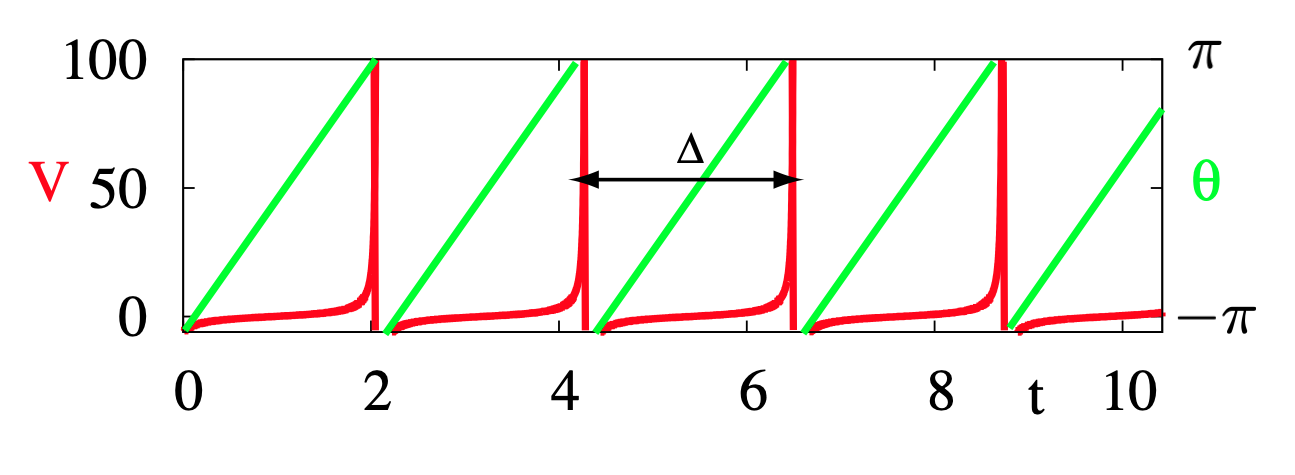
\includegraphics[width=8cm]{voltage_phase_conversion.png}
\end{figure}


Let \(\gamma(\theta)\) be the point on the limit cycle with phase
\(\theta\). For points \(x\) off of the limit cycle we can define an
\textbf{asymptotic phase}, \(\theta(x)\), as the phase along the limit
cycle to which the trajectory with initial condition \(x\) will tend as
\(t \to \infty\). The set of all points with the same asymptotic phase
define an \textbf{isochron}.

%\begin{figure}
%\centering
%\includegraphics{isochron.gif}
%\caption{isochron\_gif}
%\end{figure}

We now think about how a perturbation shifts the phase of the
oscillator. In the code above, we apply a brief negative
(hyperpolarising) current pulse. We observe that this pulse increases
the time to the next peak and we say the phase has been delayed. Let
\(\Delta_1\) be the time to the next peak. The phase shift is
\[Z(\theta) = \frac{\Delta-\Delta_1(\theta)}{\Delta}.\] Note that it
depends on the phase at which the stimulus is applied. For some values
of \(\theta\), \(Z(\theta)\) may be postive, (stimuli advance the phase,
next peak arrives sooner) and for others it may be negative (stimuli
delay the phase, next peak occurs later). We call \(Z(\theta)\) the
\textbf{phase response curve}
\href{https://en.wikipedia.org/wiki/Phase_response_curve}{(PRC)} and it
typically also depends on the form of stimulus (e.g., synaptic or gap
junction coupling). PRCs can be inferred from data or other experimental
methods. If we know the isochrons then determining the PRC is
straightforward (but in general isochrons are difficult to compute).
Note that we observed that some models have bistability between
oscillations and steady-states. The PRC is not defined for stimuli that
push the trajectory to a point where it is then not attracted back to
the oscillatory limit cycle.

    \hypertarget{infinitesimal-phase-response-curve}{%
\subsubsection{Infinitesimal phase response
curve}\label{infinitesimal-phase-response-curve}}

Suppose that the (vector) perturbation \(\delta x\) is infinitesimally
small. The associated phase shift can be approximated as
\[\delta \theta = \theta(x + \delta x) - \theta(x) = \nabla_x \theta(x) \cdot \delta x.\]
Here \(Q =\nabla_x \theta(x)\) is the gradient of the asymptotic phase
function and \((\cdot)\) is the dot product. \(Q\) is called the
infinitesimal phase response function.

\begin{quote}
\textbf{\href{https://en.wikipedia.org/wiki/Gradient}{Gradient of a
function}}: Let \(F\) be a function which takes a vector
\(\mathbf{x}= (x_1, x_2, \ldots x_n)\) and returns a scalar. Then
\[\nabla F(\mathbf{x}) = \left( \frac{\partial F}{\partial x_1}, \frac{\partial F}{\partial x_2}, \ldots, \frac{\partial F}{\partial x_n}\right)^T.\]
\end{quote}

If the unperturbed trajectory is on the limit cycle and the
perturbations are infinitesimally weak, then \(Q\) can be evaluated on
cycle and can be found numerically by solving the \textbf{adjoint}
differential equation \[ \frac{{\rm d} Q}{{\rm d}t} = - J(t)^T Q\]
subject to \(Q(t+\Delta)=Q(t)\) and \(Q(0) \cdot F(\gamma(0))= \omega\)
where \(J(t)\) is the Jacobian evaluated on the limit cycle.
\href{https://sites.pitt.edu/~phase/bard/bardware/xpp/xpp.html}{XPPAUT}
can do that for you.

 \begin{figure}[!h]
  \centering
  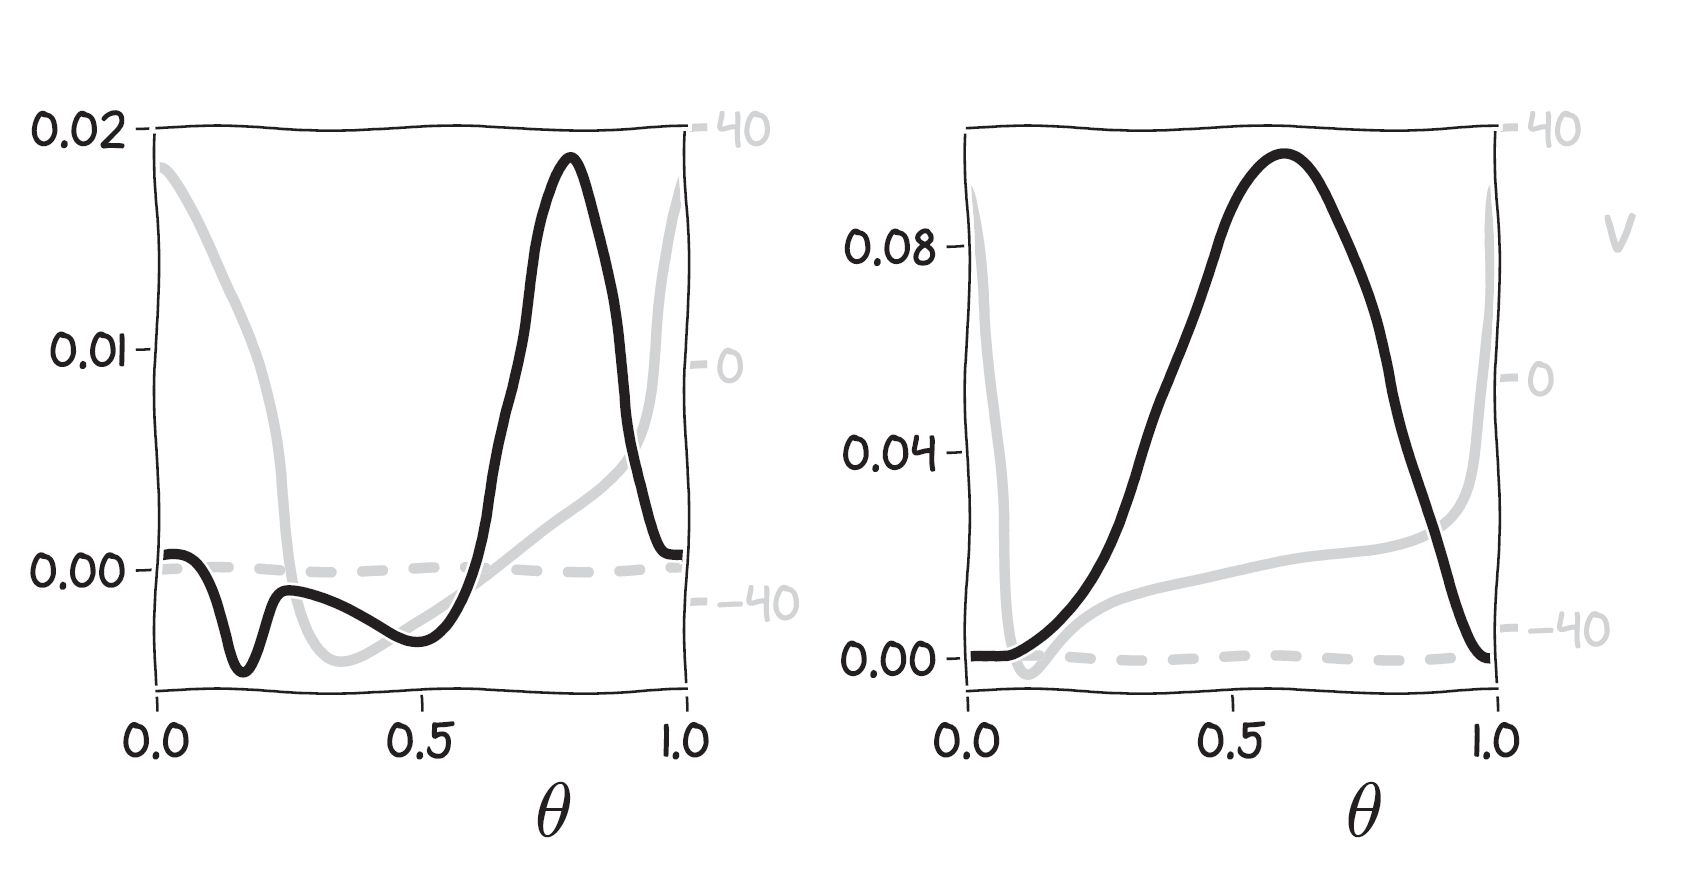
\includegraphics[width=8cm]{iPRCs.png}
\end{figure}


On the left is the first (voltage) component iPRC for Morris-Lecar near
a Hopf bifurcation (\(I=100\)) and on the right near a SNIC bifurcation
(\(I=42\)). Usually all perturbations are assumed to be in the voltage
variable. All depolarising stimuli near the SNIC lead to advancment of
the phase, whereas near the Hopf both phase advances and delays are
possible, with advances for depolarising stimuli applied during the
upstroke of the voltage on the limit cycle and delays when stimulus
occurs while \(V\) is decreasing.

    \hypertarget{phase-models}{%
\subsubsection{Phase models}\label{phase-models}}

If a weak external stimulus is applied to an oscillator
\[\frac{{\rm d} \mathbf{x}}{{\rm d} t} = \mathbf{F}(\mathbf{x}) + \epsilon \mathbf{s}(t)\]
then it can be described using phase only using the
\href{http://www.scholarpedia.org/article/Phase_model}{\textbf{phase
model}}
\[ \frac{{\rm d}\theta}{{\rm d} t} = \omega + \epsilon Q(t) \cdot \mathbf{s}(t).\]

    \hypertarget{weakly-coupled-oscillator-networks}{%
\subsection{Weakly coupled oscillator
networks}\label{weakly-coupled-oscillator-networks}}

Assume that each node in a network has a stable limit cycle in isolation
and the coupling is weak so that the trajectories of each node remain
close to their limit cycle. Then the dynamics of the network can be
captured through looking just at the phase dynamics. Consider a network
of \(N\) interacting neurons given by

\[\frac{{\rm d}\mathbf{x}_i}{{\rm d} t} = \mathbf{F}_i(\mathbf{x}_i) + \epsilon \sum_{j=1}^N w_{ij} g_{ij}(\mathbf{x}_i(t), \mathbf{x}_j(t))\]
where each isolated neuron possesses an attracting limit cycle
\(\gamma_i\) with frequency \(\omega_i\). Here \(g_{ij}\) describes the
form of the coupling between neurons \(i\) and \(j\), \(w_{ij}\)
describes the strength of interaction from node \(j\) to \(i\), while
\(\epsilon\) is an overall interaction strength. In phase-reduced form
this is

\[ \frac{{\rm d}\theta_i}{{\rm d} t} = \omega_i + \epsilon \sum_{j=1}^N w_{ij} Q_i(\theta_i) \cdot g_{ij}(\gamma_i(\theta_i), \gamma_j(\theta_j)).\tag{5}\]

Assuming identical oscillators and coupling \(Q_i = Q\) and
\(g_{ij}=g\),
\href{http://www.scholarpedia.org/article/Averaging}{Averaging Theory}
gives the evolution of the phase up to first order in \(\epsilon\) as
satisfying
\[ \frac{{\rm d}\theta_i}{{\rm d} t} = \omega_i + \epsilon \sum_{j=1}^N w_{ij} H(\theta_j - \theta_i)\]
where
\[H(\chi) = \frac{1}{2\pi} \int_0^{2\pi} Q(\phi) \cdot g(\gamma(\phi), \gamma(\phi+\chi)).\]
\href{https://sites.pitt.edu/~phase/bard/bardware/xpp/xpp.html}{XPPAUT}
can also calculate the phase interaction function \(H\) for a given
coupling function. For linear coupling in the voltage variable
\(g(\mathbf{x}_i, \mathbf{x}_j) = (v_j-v_i, 0, \ldots, 0)\) (gap
junction coupling), the phase interaction function for Morris-Lecar
neurons near a homoclinic bifurcation is on the right below with the
iPRC on the left.

 \begin{figure}[!h]
  \centering
  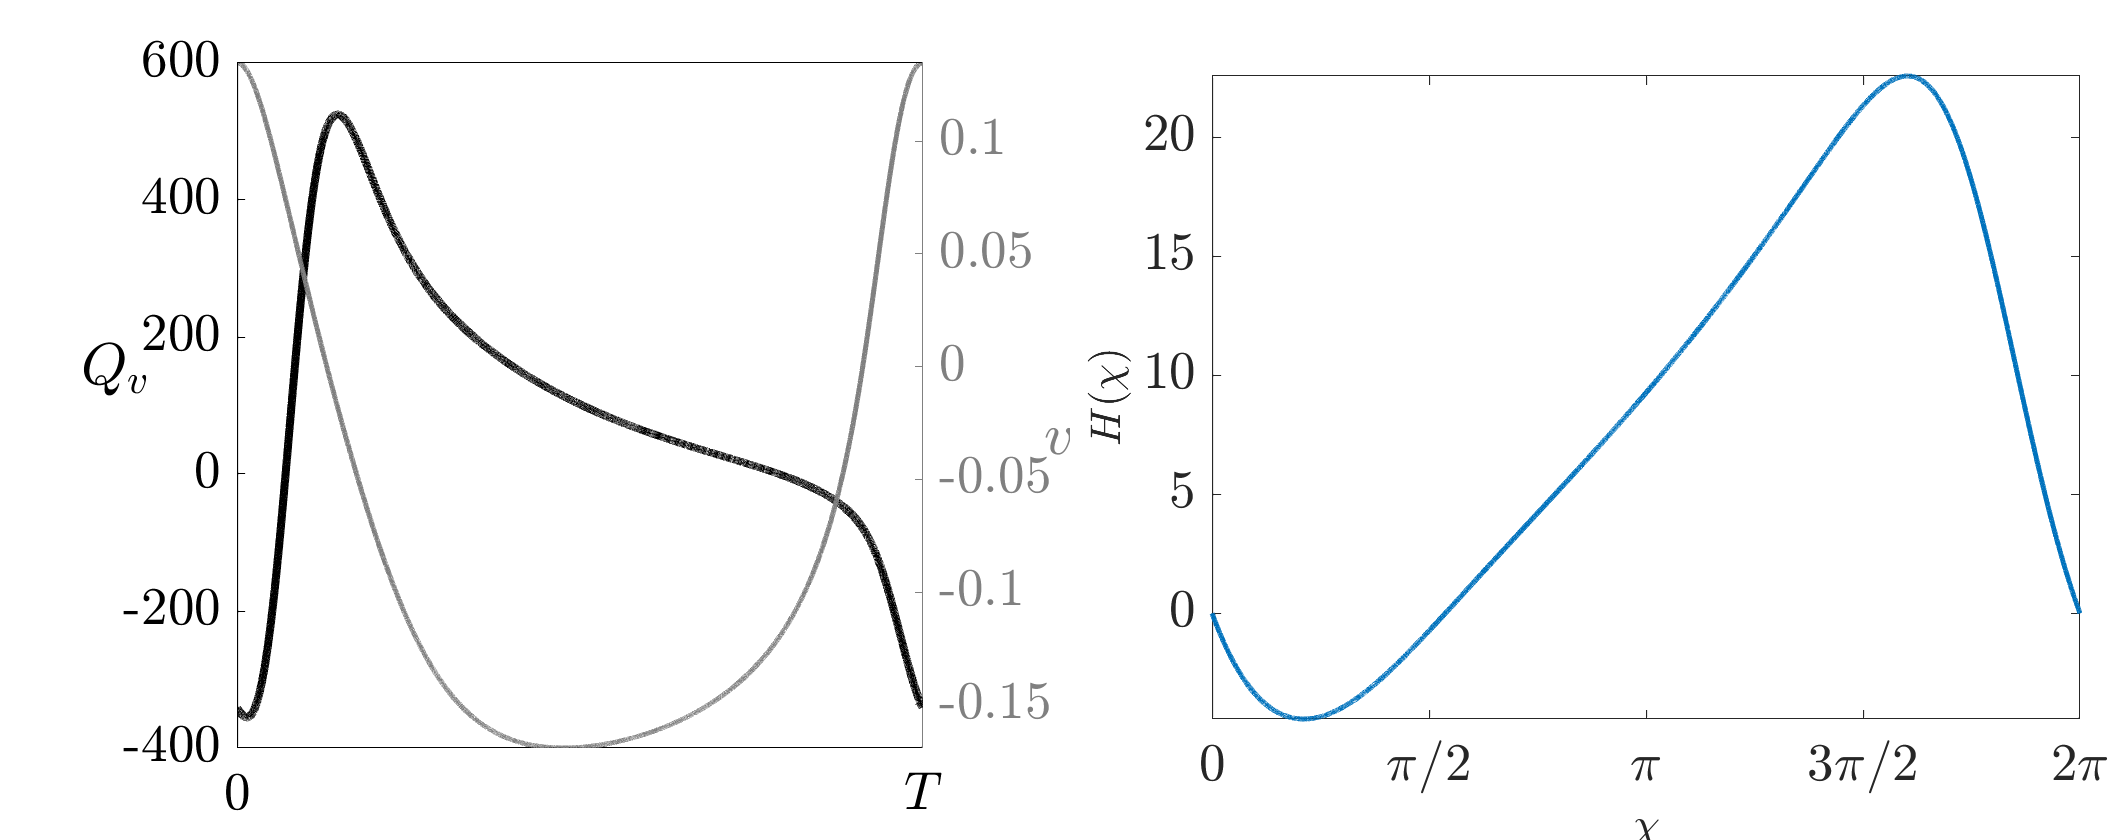
\includegraphics[width=8cm]{HML.png}
\end{figure}

The celebrated
\href{https://en.wikipedia.org/wiki/Kuramoto_model}{Kuramoto model} is
an example of this type of system with \(w_{ij}=1/N\) and
\(H(\chi) = \sin(\chi)\):

\[\frac{{\rm d}\theta_i}{{\rm d}t} = \omega_i + \frac{k}{N}\sum_{j=1}^N \sin (\theta_j-\theta_i).\]

We can run a simulation of this model with 100 nodes and frequencies
\(\omega_i\) chosen from a distribution.

    \begin{tcolorbox}[breakable, size=fbox, boxrule=1pt, pad at break*=1mm,colback=cellbackground, colframe=cellborder]
\prompt{In}{incolor}{ }{\boxspacing}
\begin{Verbatim}[commandchars=\\\{\}]
\PY{k}{def} \PY{n+nf}{kuramoto}\PY{p}{(}\PY{n}{t}\PY{p}{,}\PY{n}{x}\PY{p}{,}\PY{n}{k}\PY{p}{)}\PY{p}{:}

    \PY{n}{phase\PYZus{}diff} \PY{o}{=} \PY{n}{np}\PY{o}{.}\PY{n}{subtract}\PY{o}{.}\PY{n}{outer}\PY{p}{(}\PY{n}{x}\PY{p}{,} \PY{n}{x}\PY{p}{)}

    \PY{k}{return} \PY{n}{omega} \PY{o}{+} \PY{p}{(}\PY{n}{k}\PY{o}{/}\PY{n}{N}\PY{p}{)} \PY{o}{*} \PY{p}{(}\PY{n}{np}\PY{o}{.}\PY{n}{sin}\PY{p}{(}\PY{o}{\PYZhy{}}\PY{n}{phase\PYZus{}diff}\PY{p}{)}\PY{p}{)}\PY{o}{.}\PY{n}{sum}\PY{p}{(}\PY{n}{axis}\PY{o}{=}\PY{l+m+mi}{1}\PY{p}{)}

\PY{k+kn}{import} \PY{n+nn}{scipy}\PY{n+nn}{.}\PY{n+nn}{stats} \PY{k}{as} \PY{n+nn}{stats}

\PY{c+c1}{\PYZsh{} Define parameters}
\PY{n}{k} \PY{o}{=} \PY{l+m+mf}{0.10}
\PY{n}{N} \PY{o}{=} \PY{l+m+mi}{100}
\PY{n}{omega0} \PY{o}{=} \PY{l+m+mf}{0.5}
\PY{n}{Delta} \PY{o}{=} \PY{l+m+mf}{0.01}
\PY{n}{omega} \PY{o}{=} \PY{n}{stats}\PY{o}{.}\PY{n}{cauchy}\PY{o}{.}\PY{n}{rvs}\PY{p}{(}\PY{n}{loc}\PY{o}{=}\PY{n}{omega0}\PY{p}{,} \PY{n}{scale}\PY{o}{=}\PY{n}{Delta}\PY{p}{,} \PY{n}{size}\PY{o}{=}\PY{n}{N}\PY{p}{)}
\PY{n}{theta0} \PY{o}{=} \PY{l+m+mi}{2}\PY{o}{*}\PY{n}{np}\PY{o}{.}\PY{n}{pi}\PY{o}{*}\PY{n}{np}\PY{o}{.}\PY{n}{random}\PY{o}{.}\PY{n}{rand}\PY{p}{(}\PY{n}{N}\PY{p}{)}

\PY{c+c1}{\PYZsh{} Simulate model}
\PY{n}{kuramoto\PYZus{}sol} \PY{o}{=} \PY{n}{solve\PYZus{}ivp}\PY{p}{(}\PY{n}{kuramoto}\PY{p}{,} \PY{p}{[}\PY{l+m+mi}{0}\PY{p}{,}\PY{l+m+mi}{100}\PY{p}{]}\PY{p}{,} \PY{n}{theta0}\PY{p}{,} \PY{n}{dense\PYZus{}output} \PY{o}{=} \PY{k+kc}{True}\PY{p}{,} \PY{n}{args} \PY{o}{=} \PY{p}{(}\PY{n}{k}\PY{p}{,}\PY{p}{)}\PY{p}{)}
\PY{n}{t\PYZus{}K} \PY{o}{=} \PY{n}{np}\PY{o}{.}\PY{n}{linspace}\PY{p}{(}\PY{l+m+mi}{0}\PY{p}{,} \PY{l+m+mi}{100}\PY{p}{,} \PY{l+m+mi}{1000}\PY{p}{)}
\PY{n}{x\PYZus{}K} \PY{o}{=} \PY{n}{kuramoto\PYZus{}sol}\PY{o}{.}\PY{n}{sol}\PY{p}{(}\PY{n}{t\PYZus{}K}\PY{p}{)}\PY{o}{\PYZpc{}}\PY{p}{(}\PY{l+m+mi}{2}\PY{o}{*}\PY{n}{np}\PY{o}{.}\PY{n}{pi}\PY{p}{)}

\PY{c+c1}{\PYZsh{} Plot}
\PY{n}{plt}\PY{o}{.}\PY{n}{figure}\PY{p}{(}\PY{p}{)}
\PY{n}{plt}\PY{o}{.}\PY{n}{plot}\PY{p}{(}\PY{n}{t\PYZus{}K}\PY{p}{,} \PY{n}{x\PYZus{}K}\PY{o}{.}\PY{n}{T}\PY{p}{)}
\PY{n}{plt}\PY{o}{.}\PY{n}{xlabel}\PY{p}{(}\PY{l+s+s1}{\PYZsq{}}\PY{l+s+s1}{Time}\PY{l+s+s1}{\PYZsq{}}\PY{p}{)}
\PY{n}{plt}\PY{o}{.}\PY{n}{ylabel}\PY{p}{(}\PY{l+s+s1}{\PYZsq{}}\PY{l+s+s1}{Phase}\PY{l+s+s1}{\PYZsq{}}\PY{p}{)}
\PY{n}{plt}\PY{o}{.}\PY{n}{show}\PY{p}{(}\PY{p}{)}
\end{Verbatim}
\end{tcolorbox}

    A nicer way to visualise the evolution of the phases is to place them on
a circle

    \begin{tcolorbox}[breakable, size=fbox, boxrule=1pt, pad at break*=1mm,colback=cellbackground, colframe=cellborder]
\prompt{In}{incolor}{ }{\boxspacing}
\begin{Verbatim}[commandchars=\\\{\}]
\PY{c+c1}{\PYZsh{} Import module for animations}
\PY{k+kn}{import} \PY{n+nn}{matplotlib}\PY{n+nn}{.}\PY{n+nn}{animation} \PY{k}{as} \PY{n+nn}{ani}
\PY{c+c1}{\PYZsh{} Configure Jupyter for animated plots}
\PY{o}{\PYZpc{}}\PY{k}{matplotlib} notebook

\PY{c+c1}{\PYZsh{} Simulate the Kuramoto model}
\PY{n}{k} \PY{o}{=} \PY{l+m+mi}{1}
\PY{n}{kuramoto\PYZus{}sol} \PY{o}{=} \PY{n}{solve\PYZus{}ivp}\PY{p}{(}\PY{n}{kuramoto}\PY{p}{,} \PY{p}{[}\PY{l+m+mi}{0}\PY{p}{,}\PY{l+m+mi}{100}\PY{p}{]}\PY{p}{,} \PY{n}{theta0}\PY{p}{,} \PY{n}{dense\PYZus{}output} \PY{o}{=} \PY{k+kc}{True}\PY{p}{,} \PY{n}{args} \PY{o}{=} \PY{p}{(}\PY{n}{k}\PY{p}{,}\PY{p}{)}\PY{p}{)}
\PY{n}{x\PYZus{}K} \PY{o}{=} \PY{n}{kuramoto\PYZus{}sol}\PY{o}{.}\PY{n}{sol}\PY{p}{(}\PY{n}{t\PYZus{}K}\PY{p}{)}\PY{o}{\PYZpc{}}\PY{p}{(}\PY{l+m+mi}{2}\PY{o}{*}\PY{n}{np}\PY{o}{.}\PY{n}{pi}\PY{p}{)}

\PY{c+c1}{\PYZsh{} Set up animation}
\PY{n}{theta}\PY{o}{=}\PY{n}{np}\PY{o}{.}\PY{n}{linspace}\PY{p}{(}\PY{l+m+mi}{0}\PY{p}{,}\PY{l+m+mi}{2}\PY{o}{*}\PY{n}{np}\PY{o}{.}\PY{n}{pi}\PY{p}{,}\PY{l+m+mi}{1000}\PY{p}{)}
\PY{n}{fig}\PY{p}{,} \PY{n}{ax} \PY{o}{=} \PY{n}{plt}\PY{o}{.}\PY{n}{subplots}\PY{p}{(}\PY{n}{figsize}\PY{o}{=}\PY{p}{(}\PY{l+m+mi}{6}\PY{p}{,}\PY{l+m+mi}{6}\PY{p}{)}\PY{p}{)}

\PY{n}{ax}\PY{o}{.}\PY{n}{set\PYZus{}xlim}\PY{p}{(}\PY{p}{(}\PY{o}{\PYZhy{}}\PY{l+m+mf}{1.1}\PY{p}{,} \PY{l+m+mf}{1.1}\PY{p}{)}\PY{p}{)}
\PY{n}{ax}\PY{o}{.}\PY{n}{set\PYZus{}ylim}\PY{p}{(}\PY{p}{(}\PY{o}{\PYZhy{}}\PY{l+m+mf}{1.1}\PY{p}{,} \PY{l+m+mf}{1.1}\PY{p}{)}\PY{p}{)}
\PY{n}{line}\PY{p}{,} \PY{o}{=} \PY{n}{ax}\PY{o}{.}\PY{n}{plot}\PY{p}{(}\PY{p}{[}\PY{p}{]}\PY{p}{,} \PY{p}{[}\PY{p}{]}\PY{p}{,} \PY{l+s+s1}{\PYZsq{}}\PY{l+s+s1}{b.}\PY{l+s+s1}{\PYZsq{}}\PY{p}{,} \PY{n}{lw}\PY{o}{=}\PY{l+m+mi}{2}\PY{p}{,} \PY{n}{markersize}\PY{o}{=}\PY{l+m+mi}{10}\PY{p}{)}

\PY{k}{def} \PY{n+nf}{init}\PY{p}{(}\PY{p}{)}\PY{p}{:}
    \PY{n}{plt}\PY{o}{.}\PY{n}{plot}\PY{p}{(}\PY{n}{np}\PY{o}{.}\PY{n}{cos}\PY{p}{(}\PY{n}{theta}\PY{p}{)}\PY{p}{,}\PY{n}{np}\PY{o}{.}\PY{n}{sin}\PY{p}{(}\PY{n}{theta}\PY{p}{)}\PY{p}{,}\PY{l+s+s1}{\PYZsq{}}\PY{l+s+s1}{k\PYZhy{}\PYZhy{}}\PY{l+s+s1}{\PYZsq{}}\PY{p}{,}\PY{n}{linewidth}\PY{o}{=}\PY{l+m+mf}{0.8}\PY{p}{)}
    \PY{n}{line}\PY{o}{.}\PY{n}{set\PYZus{}data}\PY{p}{(}\PY{p}{[}\PY{p}{]}\PY{p}{,} \PY{p}{[}\PY{p}{]}\PY{p}{)}
    \PY{k}{return} \PY{p}{(}\PY{n}{line}\PY{p}{,}\PY{p}{)}

\PY{k}{def} \PY{n+nf}{dots}\PY{p}{(}\PY{n}{i}\PY{p}{)}\PY{p}{:}
    \PY{n}{x} \PY{o}{=} \PY{n}{np}\PY{o}{.}\PY{n}{cos}\PY{p}{(}\PY{n}{x\PYZus{}K}\PY{p}{[}\PY{p}{:}\PY{p}{,}\PY{n}{i}\PY{p}{]}\PY{p}{)}
    \PY{n}{y} \PY{o}{=} \PY{n}{np}\PY{o}{.}\PY{n}{sin}\PY{p}{(}\PY{n}{x\PYZus{}K}\PY{p}{[}\PY{p}{:}\PY{p}{,}\PY{n}{i}\PY{p}{]}\PY{p}{)}
    \PY{n}{line}\PY{o}{.}\PY{n}{set\PYZus{}data}\PY{p}{(}\PY{n}{x}\PY{p}{,} \PY{n}{y}\PY{p}{)}
    \PY{k}{return} \PY{p}{(}\PY{n}{line}\PY{p}{,}\PY{p}{)}

\PY{c+c1}{\PYZsh{} Create animation}
\PY{n}{animator} \PY{o}{=} \PY{n}{ani}\PY{o}{.}\PY{n}{FuncAnimation}\PY{p}{(}\PY{n}{fig}\PY{p}{,} \PY{n}{dots}\PY{p}{,} \PY{n}{init\PYZus{}func}\PY{o}{=}\PY{n}{init}\PY{p}{,} \PY{n}{interval}\PY{o}{=}\PY{l+m+mi}{100}\PY{p}{,} \PY{n}{frames}\PY{o}{=}\PY{n+nb}{range}\PY{p}{(}\PY{n+nb}{len}\PY{p}{(}\PY{n}{t\PYZus{}K}\PY{p}{)}\PY{p}{)}\PY{p}{,} \PY{n}{blit}\PY{o}{=}\PY{k+kc}{True}\PY{p}{,} \PY{n}{repeat}\PY{o}{=}\PY{k+kc}{False}\PY{p}{)}
\PY{n}{plt}\PY{o}{.}\PY{n}{show}\PY{p}{(}\PY{p}{)}
\end{Verbatim}
\end{tcolorbox}

    For weak coupling, the neurons continue to act independently. As we
increase the coupling strength, some of the slower neurons will speed up
and some of the faster neurons will slow down. This results in the
neurons \emph{synchronising} their activity. For very large values of
\(k\) all the neurons will synchronise, evolving at the same rate and
phase.

    \hypertarget{stability-of-synchrony-in-weakly-coupled-networks}{%
\subsubsection{Stability of synchrony in weakly coupled
networks}\label{stability-of-synchrony-in-weakly-coupled-networks}}

The general network equations (5) can be used to study states such as
synchrony in networks. Suppose that \(w_{ij}=1/N\), then if
\(\theta_i = \Omega t\) for a collective frequency \(\Omega\), the
oscillators are in synchrony. From (5), \(\Omega = \omega + H(0)/N.\)

The Jacobian is given by
\(J = -\epsilon \frac{{\rm d}H}{{\rm d}\chi}(0) L = -\epsilon H'(0) L\)
where \(L\) is the matrix with \(L_{ij} =\delta_{ij}-1/N\) for
\(\delta_{ij} =1\) if \(i=j\) and \(0\) otherwise. This has eigenvalues
\(1\), (\(N-1\) times) and \(0\) (corresponding to perturbations along
the periodic orbit). Therefore \(J\) has eigenvalues
\(\lambda = -\epsilon H'(0)\) and synchrony is stable if
\[\epsilon H'(0)>0.\] For positive coupling strength \(\epsilon\), phase
reduction predicts that synchrony is unstable in a network of
Morris-Lecar neurons near a homoclinic bifurcation with gap junction
coupling since the \(H\) above has negative slope at \(\chi=0\).

\hypertarget{does-this-agree-with-simulations}{%
\paragraph{Does this agree with
simulations?}\label{does-this-agree-with-simulations}}

Consider a network of two gap junction coupled Morris-Lecar neurons near
a homoclinic bifurcation:

    \begin{tcolorbox}[breakable, size=fbox, boxrule=1pt, pad at break*=1mm,colback=cellbackground, colframe=cellborder]
\prompt{In}{incolor}{ }{\boxspacing}
\begin{Verbatim}[commandchars=\\\{\}]
\PY{c+c1}{\PYZsh{} Define the ODEs}
\PY{k}{def} \PY{n+nf}{ML2}\PY{p}{(}\PY{n}{t}\PY{p}{,}\PY{n}{x}\PY{p}{,}\PY{n}{eps}\PY{p}{)}\PY{p}{:}

    \PY{n}{Va} \PY{o}{=} \PY{n}{x}\PY{p}{[}\PY{l+m+mi}{0}\PY{p}{]}
    \PY{n}{wa} \PY{o}{=} \PY{n}{x}\PY{p}{[}\PY{l+m+mi}{1}\PY{p}{]}
    \PY{n}{Vb} \PY{o}{=} \PY{n}{x}\PY{p}{[}\PY{l+m+mi}{2}\PY{p}{]}
    \PY{n}{wb} \PY{o}{=} \PY{n}{x}\PY{p}{[}\PY{l+m+mi}{3}\PY{p}{]}

    \PY{n}{m\PYZus{}infa}\PY{o}{=} \PY{l+m+mf}{0.5}\PY{o}{*}\PY{p}{(}\PY{l+m+mi}{1}\PY{o}{+}\PY{n}{np}\PY{o}{.}\PY{n}{tanh}\PY{p}{(}\PY{p}{(}\PY{n}{Va}\PY{o}{\PYZhy{}}\PY{n}{V1}\PY{p}{)}\PY{o}{/}\PY{n}{V2}\PY{p}{)}\PY{p}{)}
    \PY{n}{w\PYZus{}infa}\PY{o}{=} \PY{l+m+mf}{0.5}\PY{o}{*}\PY{p}{(}\PY{l+m+mi}{1}\PY{o}{+}\PY{n}{np}\PY{o}{.}\PY{n}{tanh}\PY{p}{(}\PY{p}{(}\PY{n}{Va}\PY{o}{\PYZhy{}}\PY{n}{V3}\PY{p}{)}\PY{o}{/}\PY{n}{V4}\PY{p}{)}\PY{p}{)}
    \PY{n}{tau\PYZus{}wa}\PY{o}{=} \PY{l+m+mi}{1}\PY{o}{/}\PY{p}{(}\PY{n}{np}\PY{o}{.}\PY{n}{cosh}\PY{p}{(}\PY{p}{(}\PY{n}{Va}\PY{o}{\PYZhy{}}\PY{n}{V3}\PY{p}{)}\PY{o}{/}\PY{p}{(}\PY{l+m+mi}{2}\PY{o}{*}\PY{n}{V4}\PY{p}{)}\PY{p}{)}\PY{p}{)}

    \PY{n}{m\PYZus{}infb}\PY{o}{=} \PY{l+m+mf}{0.5}\PY{o}{*}\PY{p}{(}\PY{l+m+mi}{1}\PY{o}{+}\PY{n}{np}\PY{o}{.}\PY{n}{tanh}\PY{p}{(}\PY{p}{(}\PY{n}{Vb}\PY{o}{\PYZhy{}}\PY{n}{V1}\PY{p}{)}\PY{o}{/}\PY{n}{V2}\PY{p}{)}\PY{p}{)}
    \PY{n}{w\PYZus{}infb}\PY{o}{=} \PY{l+m+mf}{0.5}\PY{o}{*}\PY{p}{(}\PY{l+m+mi}{1}\PY{o}{+}\PY{n}{np}\PY{o}{.}\PY{n}{tanh}\PY{p}{(}\PY{p}{(}\PY{n}{Vb}\PY{o}{\PYZhy{}}\PY{n}{V3}\PY{p}{)}\PY{o}{/}\PY{n}{V4}\PY{p}{)}\PY{p}{)}
    \PY{n}{tau\PYZus{}wb}\PY{o}{=} \PY{l+m+mi}{1}\PY{o}{/}\PY{p}{(}\PY{n}{np}\PY{o}{.}\PY{n}{cosh}\PY{p}{(}\PY{p}{(}\PY{n}{Vb}\PY{o}{\PYZhy{}}\PY{n}{V3}\PY{p}{)}\PY{o}{/}\PY{p}{(}\PY{l+m+mi}{2}\PY{o}{*}\PY{n}{V4}\PY{p}{)}\PY{p}{)}\PY{p}{)}

    \PY{n}{dVadt} \PY{o}{=} \PY{p}{(}\PY{l+m+mi}{1}\PY{o}{/}\PY{n}{C}\PY{p}{)}\PY{o}{*}\PY{p}{(}\PY{n}{I} \PY{o}{\PYZhy{}} \PY{n}{gCa}\PY{o}{*}\PY{n}{m\PYZus{}infa}\PY{o}{*}\PY{p}{(}\PY{n}{Va}\PY{o}{\PYZhy{}}\PY{n}{VCa}\PY{p}{)} \PY{o}{\PYZhy{}} \PY{n}{gK}\PY{o}{*}\PY{n}{wa}\PY{o}{*}\PY{p}{(}\PY{n}{Va}\PY{o}{\PYZhy{}}\PY{n}{VK}\PY{p}{)} \PY{o}{\PYZhy{}} \PY{n}{gL}\PY{o}{*}\PY{p}{(}\PY{n}{Va}\PY{o}{\PYZhy{}}\PY{n}{VL}\PY{p}{)}\PY{p}{)} \PY{o}{+} \PY{n}{eps}\PY{o}{*}\PY{p}{(}\PY{n}{Vb}\PY{o}{\PYZhy{}}\PY{n}{Va}\PY{p}{)}\PY{o}{/}\PY{l+m+mi}{2}
    \PY{n}{dwadt} \PY{o}{=} \PY{n}{phi}\PY{o}{*}\PY{p}{(}\PY{n}{w\PYZus{}infa}\PY{o}{\PYZhy{}}\PY{n}{wa}\PY{p}{)}\PY{o}{/}\PY{n}{tau\PYZus{}wa}
    \PY{n}{dVbdt} \PY{o}{=} \PY{p}{(}\PY{l+m+mi}{1}\PY{o}{/}\PY{n}{C}\PY{p}{)}\PY{o}{*}\PY{p}{(}\PY{n}{I} \PY{o}{\PYZhy{}} \PY{n}{gCa}\PY{o}{*}\PY{n}{m\PYZus{}infb}\PY{o}{*}\PY{p}{(}\PY{n}{Vb}\PY{o}{\PYZhy{}}\PY{n}{VCa}\PY{p}{)} \PY{o}{\PYZhy{}} \PY{n}{gK}\PY{o}{*}\PY{n}{wb}\PY{o}{*}\PY{p}{(}\PY{n}{Vb}\PY{o}{\PYZhy{}}\PY{n}{VK}\PY{p}{)} \PY{o}{\PYZhy{}} \PY{n}{gL}\PY{o}{*}\PY{p}{(}\PY{n}{Vb}\PY{o}{\PYZhy{}}\PY{n}{VL}\PY{p}{)}\PY{p}{)} \PY{o}{+} \PY{n}{eps}\PY{o}{*}\PY{p}{(}\PY{n}{Va}\PY{o}{\PYZhy{}}\PY{n}{Vb}\PY{p}{)}\PY{o}{/}\PY{l+m+mi}{2}
    \PY{n}{dwbdt} \PY{o}{=} \PY{n}{phi}\PY{o}{*}\PY{p}{(}\PY{n}{w\PYZus{}infb}\PY{o}{\PYZhy{}}\PY{n}{wb}\PY{p}{)}\PY{o}{/}\PY{n}{tau\PYZus{}wb}

    \PY{k}{return} \PY{p}{[}\PY{n}{dVadt}\PY{p}{,} \PY{n}{dwadt}\PY{p}{,} \PY{n}{dVbdt}\PY{p}{,} \PY{n}{dwbdt}\PY{p}{]}

\PY{c+c1}{\PYZsh{} Define parameters}
\PY{n}{C} \PY{o}{=} \PY{l+m+mi}{1}
\PY{n}{gCa} \PY{o}{=} \PY{l+m+mi}{1}
\PY{n}{gK} \PY{o}{=} \PY{l+m+mi}{2}
\PY{n}{gL} \PY{o}{=} \PY{l+m+mf}{0.5}
\PY{n}{VCa} \PY{o}{=} \PY{l+m+mi}{1}
\PY{n}{VK} \PY{o}{=} \PY{o}{\PYZhy{}}\PY{l+m+mf}{0.7}
\PY{n}{VL} \PY{o}{=} \PY{o}{\PYZhy{}}\PY{l+m+mf}{0.5}
\PY{n}{V1}\PY{o}{=}\PY{o}{\PYZhy{}}\PY{l+m+mf}{0.01}
\PY{n}{V2}\PY{o}{=}\PY{l+m+mf}{0.15}
\PY{n}{V3}\PY{o}{=}\PY{l+m+mf}{0.1}
\PY{n}{V4}\PY{o}{=}\PY{l+m+mf}{0.145}
\PY{n}{phi}\PY{o}{=}\PY{l+m+mf}{1.15}
\PY{n}{I} \PY{o}{=} \PY{l+m+mf}{0.075}
\end{Verbatim}
\end{tcolorbox}

    \begin{tcolorbox}[breakable, size=fbox, boxrule=1pt, pad at break*=1mm,colback=cellbackground, colframe=cellborder]
\prompt{In}{incolor}{ }{\boxspacing}
\begin{Verbatim}[commandchars=\\\{\}]
\PY{n}{eps}\PY{o}{=}\PY{l+m+mf}{0.2}
\PY{c+c1}{\PYZsh{}eps =0.8}

\PY{c+c1}{\PYZsh{} Simulate model for different initial conditions}
\PY{n}{ML2\PYZus{}sol1} \PY{o}{=} \PY{n}{solve\PYZus{}ivp}\PY{p}{(}\PY{n}{ML2}\PY{p}{,} \PY{p}{[}\PY{l+m+mi}{0}\PY{p}{,}\PY{l+m+mi}{5000}\PY{p}{]}\PY{p}{,} \PY{p}{[}\PY{o}{\PYZhy{}}\PY{l+m+mf}{0.02}\PY{p}{,}\PY{l+m+mf}{0.24}\PY{p}{,}\PY{o}{\PYZhy{}}\PY{l+m+mf}{0.05}\PY{p}{,}\PY{l+m+mf}{0.25}\PY{p}{]}\PY{p}{,} \PY{n}{dense\PYZus{}output} \PY{o}{=} \PY{k+kc}{True}\PY{p}{,} \PY{n}{args} \PY{o}{=} \PY{p}{(}\PY{n}{eps}\PY{p}{,}\PY{p}{)}\PY{p}{)}
\PY{n}{t\PYZus{}ML} \PY{o}{=} \PY{n}{np}\PY{o}{.}\PY{n}{linspace}\PY{p}{(}\PY{l+m+mi}{0}\PY{p}{,} \PY{l+m+mi}{5000}\PY{p}{,} \PY{l+m+mi}{100000}\PY{p}{)}
\PY{n}{x\PYZus{}ML21} \PY{o}{=} \PY{n}{ML2\PYZus{}sol1}\PY{o}{.}\PY{n}{sol}\PY{p}{(}\PY{n}{t\PYZus{}ML}\PY{p}{)}

\PY{n}{plt}\PY{o}{.}\PY{n}{figure}\PY{p}{(}\PY{n}{figsize}\PY{o}{=}\PY{p}{(}\PY{l+m+mi}{8}\PY{p}{,}\PY{l+m+mi}{6}\PY{p}{)}\PY{p}{)}
\PY{n}{plt}\PY{o}{.}\PY{n}{plot}\PY{p}{(} \PY{n}{t\PYZus{}ML}\PY{p}{[}\PY{l+m+mi}{98000}\PY{p}{:}\PY{p}{]}\PY{p}{,} \PY{n}{x\PYZus{}ML21}\PY{p}{[}\PY{l+m+mi}{0}\PY{p}{]}\PY{p}{[}\PY{l+m+mi}{98000}\PY{p}{:}\PY{p}{]}\PY{p}{,}\PY{n}{linewidth}\PY{o}{=}\PY{l+m+mi}{2}\PY{p}{)}
\PY{n}{plt}\PY{o}{.}\PY{n}{plot}\PY{p}{(} \PY{n}{t\PYZus{}ML}\PY{p}{[}\PY{l+m+mi}{98000}\PY{p}{:}\PY{p}{]}\PY{p}{,} \PY{n}{x\PYZus{}ML21}\PY{p}{[}\PY{l+m+mi}{2}\PY{p}{]}\PY{p}{[}\PY{l+m+mi}{98000}\PY{p}{:}\PY{p}{]}\PY{p}{,}\PY{n}{linewidth}\PY{o}{=}\PY{l+m+mi}{2}\PY{p}{)}

\PY{n}{plt}\PY{o}{.}\PY{n}{ylabel}\PY{p}{(}\PY{l+s+s2}{\PYZdq{}}\PY{l+s+s2}{membrane voltage V (mV)}\PY{l+s+s2}{\PYZdq{}}\PY{p}{)}
\PY{n}{plt}\PY{o}{.}\PY{n}{xlabel}\PY{p}{(}\PY{l+s+s2}{\PYZdq{}}\PY{l+s+s2}{time}\PY{l+s+s2}{\PYZdq{}}\PY{p}{)}
\PY{n}{plt}\PY{o}{.}\PY{n}{show}\PY{p}{(}\PY{p}{)}

\PY{c+c1}{\PYZsh{} plot trajectories in (V, w) plane}

\PY{n}{plt}\PY{o}{.}\PY{n}{figure}\PY{p}{(}\PY{n}{figsize}\PY{o}{=}\PY{p}{(}\PY{l+m+mi}{8}\PY{p}{,}\PY{l+m+mi}{6}\PY{p}{)}\PY{p}{)}
\PY{n}{plt}\PY{o}{.}\PY{n}{plot}\PY{p}{(} \PY{n}{x\PYZus{}ML21}\PY{p}{[}\PY{l+m+mi}{0}\PY{p}{]}\PY{p}{[}\PY{l+m+mi}{98000}\PY{p}{:}\PY{p}{]}\PY{p}{,} \PY{n}{x\PYZus{}ML21}\PY{p}{[}\PY{l+m+mi}{1}\PY{p}{]}\PY{p}{[}\PY{l+m+mi}{98000}\PY{p}{:}\PY{p}{]}\PY{p}{,}\PY{n}{linewidth}\PY{o}{=}\PY{l+m+mi}{2}\PY{p}{)}
\PY{n}{plt}\PY{o}{.}\PY{n}{plot}\PY{p}{(} \PY{n}{x\PYZus{}ML21}\PY{p}{[}\PY{l+m+mi}{2}\PY{p}{]}\PY{p}{[}\PY{l+m+mi}{98000}\PY{p}{:}\PY{p}{]}\PY{p}{,} \PY{n}{x\PYZus{}ML21}\PY{p}{[}\PY{l+m+mi}{3}\PY{p}{]}\PY{p}{[}\PY{l+m+mi}{98000}\PY{p}{:}\PY{p}{]}\PY{p}{,}\PY{n}{linewidth}\PY{o}{=}\PY{l+m+mi}{2}\PY{p}{)}

\PY{n}{delta} \PY{o}{=} \PY{l+m+mf}{0.025}

\PY{n}{xrange} \PY{o}{=} \PY{n}{np}\PY{o}{.}\PY{n}{arange}\PY{p}{(}\PY{o}{\PYZhy{}}\PY{l+m+mf}{0.5}\PY{p}{,} \PY{l+m+mf}{0.5}\PY{p}{,} \PY{n}{delta}\PY{p}{)}
\PY{n}{yrange} \PY{o}{=} \PY{n}{np}\PY{o}{.}\PY{n}{arange}\PY{p}{(}\PY{o}{\PYZhy{}}\PY{l+m+mf}{0.1}\PY{p}{,} \PY{l+m+mf}{0.5}\PY{p}{,} \PY{n}{delta}\PY{p}{)}
\PY{n}{Vn}\PY{p}{,} \PY{n}{wn} \PY{o}{=} \PY{n}{np}\PY{o}{.}\PY{n}{meshgrid}\PY{p}{(}\PY{n}{xrange}\PY{p}{,}\PY{n}{yrange}\PY{p}{)}

\PY{n}{F} \PY{o}{=} \PY{p}{(}\PY{l+m+mi}{1}\PY{o}{/}\PY{n}{C}\PY{p}{)}\PY{o}{*}\PY{p}{(}\PY{n}{I} \PY{o}{\PYZhy{}} \PY{n}{gCa}\PY{o}{*}\PY{l+m+mf}{0.5}\PY{o}{*}\PY{p}{(}\PY{l+m+mi}{1}\PY{o}{+}\PY{n}{np}\PY{o}{.}\PY{n}{tanh}\PY{p}{(}\PY{p}{(}\PY{n}{Vn}\PY{o}{\PYZhy{}}\PY{n}{V1}\PY{p}{)}\PY{o}{/}\PY{n}{V2}\PY{p}{)}\PY{p}{)}\PY{o}{*}\PY{p}{(}\PY{n}{Vn}\PY{o}{\PYZhy{}}\PY{n}{VCa}\PY{p}{)} \PY{o}{\PYZhy{}} \PY{n}{gK}\PY{o}{*}\PY{n}{wn}\PY{o}{*}\PY{p}{(}\PY{n}{Vn}\PY{o}{\PYZhy{}}\PY{n}{VK}\PY{p}{)} \PY{o}{\PYZhy{}} \PY{n}{gL}\PY{o}{*}\PY{p}{(}\PY{n}{Vn}\PY{o}{\PYZhy{}}\PY{n}{VL}\PY{p}{)}\PY{p}{)}\PY{p}{;}
\PY{n}{G} \PY{o}{=}  \PY{n}{phi}\PY{o}{*}\PY{p}{(}\PY{l+m+mf}{0.5}\PY{o}{*}\PY{p}{(}\PY{l+m+mi}{1}\PY{o}{+}\PY{n}{np}\PY{o}{.}\PY{n}{tanh}\PY{p}{(}\PY{p}{(}\PY{n}{Vn}\PY{o}{\PYZhy{}}\PY{n}{V3}\PY{p}{)}\PY{o}{/}\PY{n}{V4}\PY{p}{)}\PY{p}{)}\PY{o}{\PYZhy{}}\PY{n}{wn}\PY{p}{)}\PY{o}{/}\PY{p}{(}\PY{l+m+mi}{1}\PY{o}{/}\PY{p}{(}\PY{n}{np}\PY{o}{.}\PY{n}{cosh}\PY{p}{(}\PY{p}{(}\PY{n}{Vn}\PY{o}{\PYZhy{}}\PY{n}{V3}\PY{p}{)}\PY{o}{/}\PY{p}{(}\PY{l+m+mi}{2}\PY{o}{*}\PY{n}{V4}\PY{p}{)}\PY{p}{)}\PY{p}{)}\PY{p}{)}\PY{p}{;}

\PY{c+c1}{\PYZsh{}plot nullclines}
\PY{n}{plt}\PY{o}{.}\PY{n}{contour}\PY{p}{(}\PY{n}{Vn}\PY{p}{,} \PY{n}{wn}\PY{p}{,} \PY{n}{F}\PY{p}{,} \PY{p}{[}\PY{l+m+mi}{0}\PY{p}{]}\PY{p}{)}
\PY{n}{plt}\PY{o}{.}\PY{n}{contour}\PY{p}{(}\PY{n}{Vn}\PY{p}{,} \PY{n}{wn}\PY{p}{,} \PY{n}{G}\PY{p}{,} \PY{p}{[}\PY{l+m+mi}{0}\PY{p}{]}\PY{p}{)}

\PY{n}{plt}\PY{o}{.}\PY{n}{ylabel}\PY{p}{(}\PY{l+s+s2}{\PYZdq{}}\PY{l+s+s2}{Potassium gating variable (w)}\PY{l+s+s2}{\PYZdq{}}\PY{p}{)}
\PY{n}{plt}\PY{o}{.}\PY{n}{xlabel}\PY{p}{(}\PY{l+s+s2}{\PYZdq{}}\PY{l+s+s2}{membrane voltage V (mV)}\PY{l+s+s2}{\PYZdq{}}\PY{p}{)}
\PY{n}{plt}\PY{o}{.}\PY{n}{show}\PY{p}{(}\PY{p}{)}
\end{Verbatim}
\end{tcolorbox}

    For \(\epsilon\) small and positive we see that synchrony is unstable as
predicted, but as \(\epsilon\) increases, synchrony becomes stable. This
cannot be predicted using phase reduction.

    \hypertarget{beyond-phase-reduction}{%
\subsection{Beyond phase reduction}\label{beyond-phase-reduction}}

Reduction to a single phase variable for each neuron assumes that
following any perturbation the dynamics instantaneously return to the
limit cycle. This is a good approximation if the limit cycle is strongly
attracting and the perturbation is small (or coupling is weak in a
network). When this is not the case, off-cycle dynamics become important
so in addition to the phase we also include variables describing a
distance to the limit cycle which (in the absence of perturbations)
decay exponentially at rates determined by the Floquet exponents
\(\kappa_i<0\) of the stable limit cycle:

\[\frac{{\rm d} \psi_i}{{\rm d} t} = \kappa_i \psi_i\]

We call the \(\psi_i\) the amplitudes of the dynamics. Suppose for
simplicity that decay in all but one direction is fast enough to be
ignored (all but one of the \(\kappa_i\) are large and negative) and
focus only the dynamics of the most slowly decaying amplitude \(\psi\).
Each point \(x\) for which a trajectory starting from that point would
decay to the limit cycle can be assigned an amplitude. Points with equal
amplitude lie on the same \textbf{isostable} and decay to the limit
cycle in the same amount of time. On the limit cycle \(\psi=0\).

%\begin{figure}
%\centering
%\includegraphics{isostables.gif}
%\end{figure}


Just as we defined the (infinitesimal) phase response curve, we can
define the (infinitesimal) amplitude response curve. The amplitude
response to stimuli is quantified by \(I =\nabla_x \psi(x)\), the
gradient of the amplitude function. Assuming weak stimuli and evaluating
on cycle \(I\) we get the infinitesimal amplitude response curve (iARC)
which can be found as the solution of the differential equation

\[\frac{{\rm d} I}{{\rm d} t} = -(J(t) - \kappa I_n)^T I(t),\] where
\(I(t+\Delta) = I(t)\) and subject to a normalisation condition.

Then we have the phase-amplitude equations for an oscillator with time
dependent stimuli \(\epsilon \mathbf{s}(t)\):
\begin{align*} \frac{{\rm d}\theta}{{\rm d} t} &= \omega + \epsilon Q(t) \cdot \mathbf{s}(t),\\
\frac{{\rm d}\psi}{{\rm d} t} &= \kappa \psi + \epsilon I(t) \cdot \mathbf{s}(t).\end{align*}

Taking the expansions of phase and amplitude response to quadratic order
in \(\epsilon\) we get terms in the phase equation depending on
\(\psi\). Using these to describe coupled oscillator networks with
idenitcal nodes we obtain network equations which now have six
interaction functions.

\begin{align*} \frac{{\rm d}\theta_i}{{\rm d} t} &= \omega + \epsilon \sum_{j=1}^N w_{ij} \left( H_1(\theta_j -\theta_i) + \psi_i H_2(\theta_j -\theta_i) + \psi_j H_3(\theta_j -\theta_i) \right),\\
\frac{{\rm d}\psi_i}{{\rm d} t} &= \kappa \psi + \epsilon \sum_{j=1}^N w_{ij} \left( H_4(\theta_j -\theta_i) + \psi_i H_5(\theta_j -\theta_i) + \psi_j H_6(\theta_j -\theta_i) \right).\end{align*}

The stability of synchrony in a globally coupled network \(w_{ij}=1/N\)
can be considered in this framework where it is found that stability
requires
\[ \kappa + \epsilon(H_5(0) - H_1'(0))<0 ,\quad \mbox{and} \quad -\epsilon H_1'(0) \left(\kappa + \epsilon H_5(0) \right) + \epsilon^2 H_4'(0) H_2(0)>0.\]

From this, for the gap junction coupled pair of Morris-Lecar neurons, we
can predict that for some value of \(\epsilon>0\) synchrony will
restabilise.

Phase-amplitude coordinates are a promising new framework in which to
study reductions of oscillator network dynamics and can capture more of
the emergent phenomenon than phase reduction.





    % Add a bibliography block to the postdoc



\end{document}
